\NeedsTeXFormat{LaTeX2e}[1995/12/01]


% This Sample thesis requires \LaTeX2e
\NeedsTeXFormat{LaTeX2e}[1995/12/01]
%\ProvidesFile{ubcsample.tex}[2015/05/31 v1.72 ^^J
% University of British Columbia Sample Thesis]
% This is the \documentclass[]{} command.  The manditory argument
% specifies the "flavour" of thesis (ubcthesis for UBC).  The
% optional arguments (in []) specify options that affect how the
% thesis is displayed.  Please see the ubcthesis documentation for
% details about the options.
\documentclass[msc,oneside]{ubcthesis}
%\usepackage[pass,paperwidth=8.5in,paperheight=11in]{geometry}
\usepackage[
paperwidth=8.5in,
paperheight=11in,
% other options: a3paper, a5paper, etc
left=3.2cm,
right=2.5cm,
top=2.5cm,
bottom=2.5cm,
% use vmargin=2cm to make vertical margins equal to 2cm.
% us  hmargin=3cm to make horizontal margins equal to 3cm.
% use margin=3cm to make all margins  equal to 3cm.
]
{geometry}
%\pdfpageheight=11in
%\pdfpagewidth=8.5in
%
% To compile this sample thesis, issue the following commands:
% latex ubcsample
% bibtex ubcsample
% latex ubcsample
% latex ubcsample
% latex ubcsample
%
% To view use xdvi (on unix systems):
% xdvi ubcsample.dvi
%
% To make a postscript file, use dvips:
% dvips -o ubcsample.ps ubcsample.dvi
%
% To view the postscript file, use ghostview or gv (on unix systems):
% gv ubcsample.ps
%
%************************************************
% Optional packages.
%
% The use of these packages is optional, but they provide various
% tools for more flexible formating.  The sample thesis uses these,
% but if you remove the example code, you should be able to exclude
% these packages.  Only standard packages have been described here;
% they should be installed with any complete LaTeX instalation, but
% if not, you can find them at the Comprehensive TeX Archive Network
% (CTAN): http://www.ctan.org/
%

%******** afterpage ***************************
% This package allows you to issue commands at the end of the current
% page.  A good use for this is to use the command
% \afterpage{\clearpage} right after a figure.  This will cause the
% figure to be inserted on the page following the current one (or on
% the current page if it will fit) but will not break the page in the
% middle.
\usepackage{afterpage}
\usepackage{xcolor}
%******** float *********************************
% This package allows you to customize the style of
% "floats"---floating objects such as figures and tables.  In
% addition, it allows you to define additional floating objects which
% may be included in a list similar to that produces by \listoftables
% and \listoffigures.  Common uses include introducing floats for
% programs and other code bits in Compute Science and Chemical Schema.
\usepackage{float}
\usepackage{amsmath,bm}
\usepackage{tikz}
\usepackage{quantikz}
\usepackage{tabularray}
\usepackage{dsfont}
\usepackage{booktabs} % For professional looking tables
\usepackage{multirow} % Required for combining rows
\usepackage{amsfonts}
\usepackage{caption}
\usepackage{subcaption}
\usetikzlibrary{shapes.geometric}
\usetikzlibrary{arrows.meta} % For arrow tips
\usepackage{xcolor} % For colors
\definecolor{lightblue}{RGB}{173,216,230} % Define light blue
%******** tocloft *******************************
% This package allows you to customize and define custom lists such
% as a list of programs or Chemical Scheme.  Note: if you use the
% subfigure package, you must specify that you do as an option here.
% The title option uses the default formatting.  We do not use this
% here as the default formatting is acceptable.  Use the float
% package instead unless you need the extra formatting control
% provided by tocloft.
%\usepackage[subfigure, titles]{tocloft}

%******** alltt *********************************
% The alltt package allows you to include files and have them
% formatted in a verbatim fashion.  This is useful for including
% source code from an additional file.
%\usepackage{alltt}

%******** listings ******************************
% The listings package may be used to include chunks of source code
% and has facilities for pretty-printing many languages.
%\usepackage{listings}

%******** longtable *****************************
% The longtable package allows you to define tables that span
% multiple pages.



\usepackage{longtable}

%******** graphics and graphicx *****************
% This allows you to include encapsulated postscript files.  If you
% don't have this, comment the \includegraphics{} line following the
% comment "%includegraphics" later in this file.
\usepackage{graphicx}

%******** subfigure *****************************
% The subfigure package allows you to include multiple figures and
% captions within a single figure environment.
%\usepackage{subfigure}

%******** here **********************************
% The here package gives you more control over the placement of
% figures and tables.  In particular, you can specify the placement
% "H" which means "Put the figure here" rather than [h] which means
% "I would suggest that you put the figure here if you think it looks
% good."
%\usepackage{here}

%******** pdflscape ********************************
% This allows you to include landscape layout pages by using the
% |landscape| environment.  The use of |pdflscape| is preferred over
% the standard |lscape| package because it automatically rotates the
% page in the pdf file for easier reading.  (Thanks to Joseph Shea
% for pointing this out.)
\usepackage{pdflscape}
\usepackage{pdfpages}
\usepackage{xcolor}

%******** natbib ********************************
% This is a very nice package for bibliographies.  It includes options
% for sorting and compressing bibliographic entries.
\usepackage[numbers,sort&compress]{natbib}
%\usepackage{natbib}   % omit 'round' option if you prefer square brackets

%\usepackage{hyperref}
\usepackage[unicode=true,
colorlinks=true,
linktocpage,
linkbordercolor={0.5 0.5 1},
citebordercolor={0.5 1 0.5},
linkcolor=blue]{hyperref}


\usepackage[nameinlink]{cleveref}


% for clever referencing, i.e. references equations as e.g.: eq. (1.1), particularly useful together with hyperref (which is automatically loaded by jcappub)

%******** psfrag ******************************
% This allows you to replace text in postscript pictures with formated
% latex text.  This allows you to use math in graph labels
% etc. Uncomment the psfrag lines following the "%psfrag" comment
% later in this file if you don't have this package.  The replacements
% will only be visible in the final postscript file: they will be
% listed in the .dvi file but not performed.
%\usepackage{psfrag}
%\usepackage[margin=0.5in]{geometry}
%******** hyperref *****************************
% Please read the manual:
% http://www.tug.org/applications/hyperref/manual.html
%
% This adds hyperlinks to your document: with the right viewers (later
% versions of xdvi, acrobat with pdftex, latex2html etc.) this will
% make your equation, figure, citation references etc. hyperlinks so
% that you can click on them.  Also, your table of contents will be
% able to take you to the appropriate sections.  In the viewers that
% support this, the links often appear with an underscore.  This
% underscore will not appear in printed versions.
%
% Note: if you do not use the hypertex option, then the dvips driver
% may be loaded by default.  This will cause the entries in the list
% of figures and list of tables to be on a single line because dvips
% does not deal with hyperlinks on broken lines properly.
%
% NOTE: HYPERREF is sensitive to the ORDER in which it is LOADED.
% For example, it must be loaded AFTER natbib but BEFORE newly
% defined float environments.  See the README file with the hyperref
% for some help with this.  If you have some very obscure errors, try
% first disabling hyperref.  If that fixes the problem, try various
% orderings.
%
% Note also that there is a bug with versions before 2003/11/30
% v6.74m that cause the float package to not function correctly.
% Please ensure you have a current version of this package.  A
% warning will be issued if you leave the date below but do not have
% a current version installed.
%
% Some notes on options: depending on how you build your files, you
% may need to choose the appropriate option (such as [pdftex]) for the
% backend driver (see the hyperref manual for a complete list).  Also,
% the default here is to make links from the page numbers in the table
% of contents and lists of figures etc.  There are other options:
% excluding the [linktocpage] option will make the entire text a
% hyperref, but for some backends will prevent the text from wrapping
% which can look terrible.  There is a [breaklinks=true] option that
% will be set if the backend supports (dvipdfm for example supports
% it but does not work with psfrag.)
%
% Finally, there are many options for choosing the colours of the
% links.  These will be included by default in future versions but
% you should probably consider changing some now for the electronic
% version of your thesis.
%\usepackage[unicode=true,
%  linktocpage,
%  linkbordercolor={0.5 0.5 1},
%  citebordercolor={0.5 1 0.5},
%  linkcolor=blue]{hyperref}

% If you would like to compile this sample thesis without the
% hyperref package, then you will need to comment out the previous
% \usepackage command and uncomment the following command which will
% put the URL's in a typewriter font but not link them.
%\newcommand\url[1]{\texttt{#1}}

%******** setspace *******************************
% The setspace package allows you to manually set the spacing of the
% file.  UBC may require 1.5 spacing for microfilming of theses.  In
% this case you may obtain this by including this package and issuing
% one of the following commands:
%\usepackage{setspace}
%\singlespacing
%\onehalfspacing
%\doublespacing

% These commands are optional.  The defaults are shown.  You only
% need to include them if you need a different value
\institution{The University Of British Columbia}

% If you are at the Okanagan campus, then you should specify these
% instead.
%\faculty{The College of Graduate Studies}
%\institutionaddress{Okanagan}
\faculty{The Faculty of Science}
\institutionaddress{Vancouver}

% You can issue as many of these as you have...
%\previousdegree{B.Sc., University of British Columbia, year}
%\previousdegree{M.Sc., The University of British Columbia, 2022}
%\previousdegree{Ph.D., Massachusetts Institute of Technology, 2005}

% You can override the option setting here.
\degreetitle{Bachelor of Science}

% These commands are required.
\title{A Quantum Algorithm for the Bottleneck Travelling Salesman Problem}
%\subtitle{With a Subtitle}
\author{Raveel Tejani}
%\copyrightyear{2000}
\submitdate{\monthname\ \number\year} % The "\ " is required after
% \monthname to prevent the
% command from eating the space.
\program{Physics}

% These commands are presently not required for UBC theses as the
% advisor's name and title are not presently required anywhere.
%\advisor{Ariel R.~Zhitnitsky}
%\advisortitle{Professor of Physics}

% One might want to override the format of the section and chapter
% numbers.  This shows you how to do it.  Note that the current
% format is acceptable for submission to the FoGS: If you wish to modify
% these, you should check with the FoGS explicity. prior to making
% the modifications.
\renewcommand\thepart         {\Roman{part}}
\renewcommand\thechapter      {\arabic{chapter}}
\renewcommand\thesection      {\thechapter.\arabic{section}}
\renewcommand\thesubsection   {\thesection.\arabic{subsection}}
\renewcommand\thesubsubsection{\thesubsection.\arabic{subsubsection}}
\renewcommand\theparagraph    {\thesubsubsection.\arabic{paragraph}}
\renewcommand\thesubparagraph {\theparagraph.\arabic{subparagraph}}

\setcounter{tocdepth}{2}
\setcounter{secnumdepth}{2}
%\newcommand{\arefe}[1]{{\textcolor{cyan}{#1}}}
% Here is an example of a "Program" environment defined with the
% "float" package.  The list of programs will be stored in the file
% ubcsample.lop and the numbering will start with the chapter
% number.  The style will be "ruled".
\floatstyle{ruled}
\newfloat{Program}{htbp}{lop}[chapter]






%%%%%%%%%%%%%%%%%%%%%%%%%%%%%%%%%%%%%%%%%%%%%%%%%%%%%%%%%%%%
%EVERTYTHING FOR JUPYTER NOTEBOOK%%%%%




%%%%%%%%%%%%%%%%%%%%%%%%%%%%%%%%%%%%%%%%%%%%%%%%%%%%%%%%%%%%%
% Here is the start of the document.
\begin{document}
	
	
	\frontmatter

	\maketitle               
	

	\clearpage
	\begin{abstract}                %% Mandatory -  maximum 350 words
%		The \texttt{genthesis.cls} \LaTeX{} class file and accompanying
%		documents, such as this sample thesis, are distributed in the hope
%		that it will be useful but without any warranty (without even the
%		implied warranty of fitness for a particular purpose).  For a
%		description of this file's purpose, and instructions on its use, see
%		below.
%		
		%We present  a constraint and full solution to the bottleneck travelling salesman problem based on the quantum phase estimation algorithm.
		
		We develop a quantum algorithm leveraging quantum phase estimation to address the decision problem variant of the Bottleneck Travelling Salesman Problem. This algorithm's efficacy is evaluated through diverse orders of phase estimation applied to both 4-city and 5-city graphs. While the algorithm preserves the original complexity of the problem, $O((N-1)!)$, we introduce a strategy for parallelization, enabling simultaneous execution across all Hamiltonian cycles.
		
		\textbf{probably need more text here.}
	\end{abstract}
	
	
	\tableofcontents %% Mandatory
	\listoftables                   %% Mandatory if thesis has tables
	\listoffigures                  %% Mandatory if thesis has figures

	
	\chapter{Acknowledgements} 
	
	
	I want to express my gratitude to Prof. Matthew Choptuik for not only his supervision but also for the encouragement and support to pursue a topic that truly captivates my interest. I would like to thank Erin Bennett and Jason Li, my fellow physics undergrads for getting me through school. I would also like to thank Stefan Grahovac for keeping me motivated  and cheering me on through my degree. Finally, I would like to thank my parents for their support and my sister, Mehak Tejani, for enjouraging me to pursue physics.
	
	
	\mainmatter
	
	\chapter{Introduction}

	
	
Continuous advancements in quantum computing have allowed for contemporary approaches to solve complex computational problems that were previously considered intractable using classical methods. Well known examples of these advancements include Shor's \cite{Shor} and Grover's \cite{grover1996fast} algorithms for factoring and unstructured search respectively. The Bottleneck Traveling Salesman Problem (BTSP) serves as a challenging optimization problem in the field of logistics and operations research. Its practical applications range from optimizing vehicle routes, to circuit design. Consequently, the achievement of an efficient solution is highly sought after. However, the BTSP is classified as an NP-hard problem, indicating it is at least as difficult as the hardest problems in the NP class. For reference, an NP problem must satisfy two conditions: no known solution in polynomial time, and the verification of a solution in polynomial time. An NP-hard problem does not need to satisfy the verification condition. To address this problem, many heuristic approaches are explored \cite{heuristicthesis}\cite{heuristic}. However, inherent to such methods is a trade-off between precision and efficiency.

We embark on a journey at the intersection of quantum computing and optimization by introducing a quantum algorithm tailored to address the BTSP. It requires finding a closed tour through a set of cities while minimizing the largest cost, the "bottleneck", along any route. Its computational complexity grows exponentially with the number of cities, rendering classical solutions impractical for large-scale instances. Our approach is to capitalize on the inherent quantum parallelism, as well as the unique feature of phase encoding in quantum computing. By exploiting these phenomena, we aim to encode and manipulate the costs associated with various routes efficiently. 

In the upcoming chapter, we delve into the complexities of the BTSP. We will then explore quantum computing fundamentals and progress to an in-depth discussion on quantum phase estimation. We follow this with a detailed explanation of our proposed algorithm as well as run various simulations. Finally, we will discuss the benefits and drawbacks of our algorithm in the context of the results from the simulations.
	
	\chapter{Theory}
	\section{The Bottleneck Travelling Salesman Problem}


\begin{figure}[!h]
	\centering
	\includegraphics[trim={0 0 21.9cm 0},clip, width=0.4 \linewidth]{"graphics/4-city"}
	\caption{An undirected weighted graph represention of a  symmetric 4-city system.  The vertices represent cities and the edge weights represent the cost of travel. }
	\label{fig:4-city-graphic}
\end{figure}		

We start with a graph, whose vertices are labelled A through D, representing a 4-city system. We define movement from one vertex to another as a walk, done through the edges connecting our vertices. We are interested in a particular walk known as a Hamiltonian cycle that contains every vertex exactly once before returning to the start. Our graph also includes edge weights, we define as $ \gamma_i $.
The BTSP is to find the Hamiltonian cycle in a graph, where the largest edge weight (bottleneck) is minimized. This is distinct from the Travelling Salesman Problem (TSP) where the combined edge weights in a given cycle is minimized. The total possible Hamiltonian cycles is given by $(N-1)!$, where N is the number of nodes. We present a symmetric case in FIG .\ref{fig:4-city-graphic},  $N_k \rightarrow N_{k+1} = N_{k+1} \rightarrow N_{k} = \gamma_i$. Thus the total possible cycles is  $(N-1)!/2$.  It is important to note that a solution to either BTSP or TSP is not unique. Moreover, BTSP solutions do not necessarily equate to the TSP solutions. We can illustrate an example below. Consider all the Hamiltonian cycles for a symmetric 4-city system:

\begin{center}
	$ A \rightarrow B \rightarrow C \rightarrow D \rightarrow A $
	
	$ A \rightarrow B \rightarrow D \rightarrow C \rightarrow A $ 
	
	$ A \rightarrow C \rightarrow B \rightarrow D \rightarrow A $
\end{center}

Assigning some arbitrary weights, we can see the total costs of the cycles below. The first cycle is the solution to the BTSP as its largest edge weight at $5$ is the smallest among all three. The last cycle is a solution to the TSP as its combined edge weight is the smallest.
\begin{center}
	$\gamma_1 + \gamma_4 + \gamma_5 + \gamma_3 = 4 + 4 + 5 + 4 = 17$
	
	$ \gamma_1 + \gamma_6 + \gamma_5 + \gamma_2 = 4 + 6 + 5 + 2 = 17$
	
	$  \gamma_2 + \gamma_4 + \gamma_6 + \gamma_3 = 2 + 4 + 6 + 4 = 16$
\end{center}


By simply changing the weight of $\gamma_6$ to $5$, we can illustrate that all cycles are solutions to the BTSP. 

\begin{center}
	
	$\gamma_1 + \gamma_4 + \gamma_5 + \gamma_3 = 4 + 4 + 5 + 4 = 17$
	
	$ \gamma_1 + \gamma_6 + \gamma_5 + \gamma_2 = 4 + 5 + 5 + 2 = 16$
	
	$  \gamma_2 + \gamma_4 + \gamma_6 + \gamma_3 = 2 + 4 + 5 + 4 = 15$
\end{center}

The computational complexity of the BTSP is known to be NP-hard, implying there is no algorithm for a solution in polynomial time. A brute-force approach would imply that we can run an algorithm in $\mathcal{O}((N-1)!)$ time.
	
	\section{An Introduction to Quantum Computing}
	
	Quantum computing represents a fundamentally different approach to computation compared to  it's classical counterpart. At its core, quantum computing leverages principles of quantum physics to process information in ways that classical computers can't. Let us look at some key differences:
	\begin{enumerate}
		\item 	Information Representation: Classical bits are binary and can only be in one state at a time (0 or 1). Qubits, however, can be in a superposition of the basis states.

		\item 	Determinism: Classical computing is deterministic, implying the output of a computation is predictable if you know the input and the algorithm. Quantum computing, however, is probabilistic. Only after measurement we achieve a deterministic reading. This means that quantum algorithms can give different outcomes with each run with respect to their probabilites.
		
		\item Operations: Classical computers perform operations using logical gates (AND, OR, NOT). In quantum computers perform operations using unitary operators that define quantum logic gates. Unitary operators satisfy the condition $U^{\dagger}U = \mathbb{I}$. This implies all quantum operations are reversible, which is not generally the case in classical computation.
		
	\end{enumerate}
	
	
	\subsection{Frequently Used Notation}
	
	Let us start by looking at single qubit states, these are, by convention, in the computational basis: 
	\begin{align*}	
		|0\rangle &= \begin{bmatrix}
			1 \\
			0 \\
		\end{bmatrix}, 
		|1\rangle = \begin{bmatrix}
			0 \\
			1 \\
		\end{bmatrix}
	\end{align*}
	
	We can have a superposition of basis states:
	
	$$|s\rangle = \alpha|0\rangle + \beta|1\rangle$$
	
	Were: $|\alpha|^2$ represents the probability of measuring state $|0\rangle$,  and $|\beta|^2 $ represents the probability of measuring state $|1\rangle$. Thus our amplitudes should satisfy the condition:
	
	$$|\alpha|^2 + |\beta|^2 = 1$$
	
	Below we can see the Pauli-X gate, and we can see the result on the single qubit states is analogous to the NOT gate in classical computation.
	
		\begin{align*}	
		X &= \begin{bmatrix}
			0 & 1 \\
			1 &0 \\
		\end{bmatrix}
	\end{align*}
	
	\begin{align*}	
		X|0\rangle = |1\rangle\\
		X|1\rangle = |0\rangle
	\end{align*}
	
	
	Below we can see the Hadamard gate and the result of its application to single qubit states, frequently employed to establish a uniform superposition.

	
	\begin{align*}	
		H &=\frac{1}{\sqrt{2}} \begin{bmatrix}
			1 & 1 \\
			1 &-1 \\
		\end{bmatrix}
	\end{align*}
	
	\begin{align*}	
		H|0\rangle = \frac{1}{\sqrt{2}} (|0\rangle + |1\rangle) = |+\rangle\\
		H|1\rangle = \frac{1}{\sqrt{2}} (|0\rangle - |1\rangle) = |-\rangle
	\end{align*}
	
	
	Multiple qubit states are achieved through tensor products of single states. An $n$-qubit system will span a Hilbert space $N = 2^n $. We can see with the $2$-qubit system we have $4$ states. 
	
	\begin{align*}	
		|00\rangle &= |0\rangle \otimes |0\rangle = \begin{bmatrix}
			1 \\
			0 \\
			0 \\
			0 \\
		\end{bmatrix}, 
		|01\rangle = |0\rangle \otimes |1\rangle = \begin{bmatrix}
			0 \\
			1 \\
			0 \\
			0 \\
		\end{bmatrix} 			
	\end{align*}
	
	\begin{align*}	
		|00\rangle &= |1\rangle \otimes |0\rangle = \begin{bmatrix}
			0 \\
			0 \\
			1 \\
			0 \\
		\end{bmatrix}, 
		|01\rangle = |1\rangle \otimes |1\rangle = \begin{bmatrix}
			0 \\
			0 \\
			0 \\
			1 \\
		\end{bmatrix}		
	\end{align*}
	
 The Hadamard gate can also be extended to multiple qubit states. Let us see it applied to $|00\rangle$:
	
	\begin{align*}	
		H^{\otimes 2}|00\rangle &= H|0\rangle H|0\rangle\\
		&= |+\rangle|+\rangle\\
		&= (\frac{1}{\sqrt{2}} (|0\rangle + |1\rangle))(\frac{1}{\sqrt{2}} (|0\rangle + |1\rangle))\\
		&= \frac{1}{2} (|0\rangle + |1\rangle)(|0\rangle + |1\rangle)\\
		&= \frac{1}{2} (|00\rangle + |01\rangle + |10\rangle + |11\rangle)\\
	\end{align*}
	
	\subsection{Quantum Circuit Components}
	
	We can represent unitary operations on qubits through quantum circuit diagrams similiar to classical circuits. Frequently used circuit components are listed below:
	
	\begin{center}
		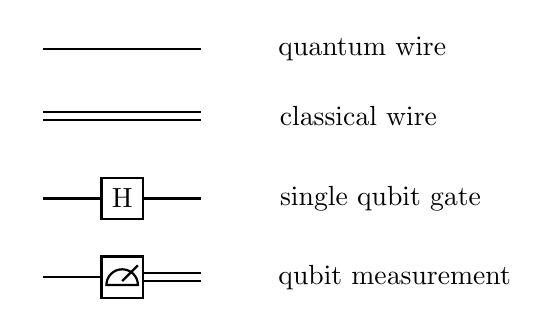
\begin{tikzpicture}[thick]
			
			\tikzstyle{operator} = [draw,fill=white,minimum size=1.5em] 
			
			%\draw (3,3) -- (3,0) ;
			
			\draw (0,3) -- (2,3) ;
			\node at (4.05,3) {quantum wire};
			
			\draw (0,2.1) -- (2,2.1) ;
			\draw (0,2.2) -- (2,2.2) ;
			\node at (4,2.15) {classical wire};
			
			\draw (0,1.1) -- (2,1.1) ;
			\node[operator] (op11) at (1,1.1) {H};
			\node at (4.28,1.1) {single qubit gate};
			
			\draw (0,0.1) -- (1,0.1) ;
			
			\draw (1,0.15) -- (2,0.15) ;
			\draw (1,0.05) -- (2,0.05) ;
			% Define coordinates
			\def\Radius{0.2}
			\path
			(-\Radius, 0) coordinate (A)
			-- coordinate (M)
			(\Radius, 0) coordinate (B)
			(M) +(60:\Radius) coordinate (C)
			+(120:\Radius) coordinate (D)
			;
			
			\node[operator] (op11) at (1,0.1) {};
			\node at (4.46,0.1) {qubit measurement};
			
			% Draw semicircle
			\draw[operator]
			(1.2,0) arc(0:180:\Radius) -- cycle ;
			% Annotations
			
			\draw (1,0.05) -- (1.2,0.25);
			
		\end{tikzpicture}
\end{center}
	
	\subsection{Controlled Gates}
	
	A controlled gate operates on two or more qubits, where one or more qubits act as the "control" qubits, and the others as the "target" qubit. For the context of this thesis, we will discuss controlled operations in the context of a single control qubit.
	
	Let us start with the controlled-$X$ gate. Below we can see the quantum circuit and matrix representation as well as its affect on all 2-qubit states:
	
	\begin{figure}[!h]
		\centering
		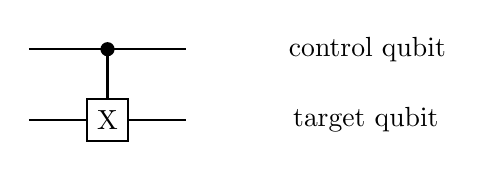
\begin{tikzpicture}[thick]
			
			\tikzstyle{operator} = [draw,fill=white,minimum size=1.5em] 
			
			%\draw (3,3) -- (3,0) ;
			
			\draw (0,2) -- (2,2) ;
			\node at (4.30,2) {control qubit};
			
			\draw[black,fill=black] (1,2) circle (.5ex);
			\draw (1, 1.1) -- (1, 2);
			
			\draw (0,1.1) -- (2,1.1) ;
			\node[operator] (op11) at (1,1.1) {X};
			\node at (4.28,1.1) {target qubit};
		\end{tikzpicture}
	\end{figure}	

	
	\begin{align*}	
		CX &= 	\begin{bmatrix}
			\mathbb{I}_2 & 0 \\
			0 & X \\
		\end{bmatrix}= \begin{bmatrix}
		1 & 0 & 0 & 0  \\
		0 &1 & 0 &0 \\
		0 &0 & 0 & 1 \\
		0 &0 & 1 & 0 \\
		\end{bmatrix}
	\end{align*}
	
	\begin{align*}	
		X|00\rangle &= |00\rangle\\
		X|01\rangle &= |01\rangle\\
		X|10\rangle &= |11\rangle\\
		X|11\rangle &= |10\rangle
	\end{align*}
	
	In this operation, only the only the states $|10\rangle$ and $|11\rangle$ undergo any change. The first qubit, positioned on the left, serves as the control qubit, determining whether the operation is applied. The second qubit, on the right, is the target qubit that is only affected if the control qubit is in state $|1\rangle$.
	
	Let us now look at the controlled-$Z$ gate. Again, we can look at the quantum circuit and matrix representation as well as its affect on all 2-qubit states.
	
	
		\begin{figure}[!h]
		\centering
		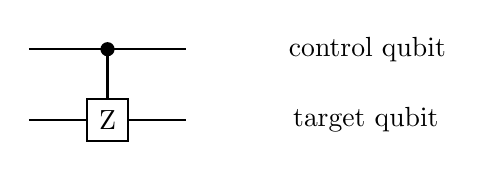
\begin{tikzpicture}[thick]
			
			\tikzstyle{operator} = [draw,fill=white,minimum size=1.5em] 
			
			%\draw (3,3) -- (3,0) ;
			
			\draw (0,2) -- (2,2) ;
			\node at (4.30,2) {control qubit};
			
			\draw[black,fill=black] (1,2) circle (.5ex);
			\draw (1, 1.1) -- (1, 2);
			
			\draw (0,1.1) -- (2,1.1) ;
			\node[operator] (op11) at (1,1.1) {Z};
			\node at (4.28,1.1) {target qubit};
		\end{tikzpicture}
	\end{figure}	
	
	
	\begin{align*}	
		CZ &= 	\begin{bmatrix}
			\mathbb{I}_2 & 0 \\
			0 & Z \\
		\end{bmatrix}= \begin{bmatrix}
			1 & 0 & 0 & 0  \\
			0 &1 & 0 &0 \\
			0 &0 & 1 & 0 \\
			0 &0 & 0 & -1 \\
		\end{bmatrix}
	\end{align*}
	
	\begin{align*}	
		Z|00\rangle &= |00\rangle\\
		Z|01\rangle &= |01\rangle\\
		Z|10\rangle &= |10\rangle\\
		Z|11\rangle &= -|11\rangle
	\end{align*}
	
	We can see in this case, only the final state, $|11\rangle$ was affected and it specifically altered the state's phase.  We can construct our own controlled gates with any unitary matrix $U$. A controlled-$U$ designed to act on $n$ target qubits,  can be represented in block matrix notation. In this framework, $\mathbb{I}_n$ refers to the identity matrix with $2^{n}$ diagonal elements:
	
		\begin{figure}[!h]
		\centering
		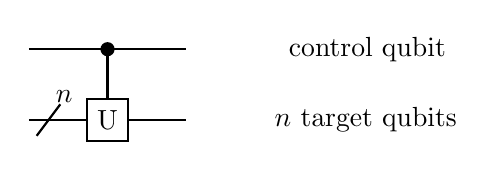
\begin{tikzpicture}[thick]
			
			\tikzstyle{operator} = [draw,fill=white,minimum size=1.5em] 
			
			%\draw (3,3) -- (3,0) ;
			
			\draw (0,2) -- (2,2) ;
			\node at (4.30,2) {control qubit};
			
			\draw[black,fill=black] (1,2) circle (.5ex);
			\draw (1, 1.1) -- (1, 2);
			
			\draw (0,1.1) -- (2,1.1) ;
			\node[operator] (op11) at (1,1.1) {U};
			\node at (4.28,1.1) {$n$ target qubits};
			
			\draw (0.1,0.9) -- (0.4,1.3) ;
			\node at (0.45,1.4) {$n$};
		\end{tikzpicture}
	\end{figure}	
	
	
	\begin{equation}\label{control-u-matrix}
	CU = \begin{bmatrix}
		\mathbb{I}_n & 0 \\
		0 & U \\
	\end{bmatrix}
	\end{equation}

	
	\section{Quantum Phase Estimation}
			The phase estimation algorithm initially proposed by Alexey Kitaev \cite{kitaev1995quantum} plays an important role as a subroutine for the more widely known factoring algorithm by Peter Shor \cite{Shor}. We first must briefly discuss the Quantum Fourier Transform (QFT) as it is key to understanding phase estimation \cite{nielsen00}. Given a computational basis state $|x\rangle$, applying the QFT ($F_N$) results in:
	
	$$ F_N |x \rangle = \frac{1}{\sqrt{N}} \sum_{k=0}^{N-1} e^{2\pi i x k N^{-1}} |k\rangle $$
	
	Let us represent this in binary notation and decompose it into a tensor product. We can represent $|x\rangle$ as a string of bits, and the QFT as a tensor product of single qubit basis states:
	
	$$|x\rangle = |x_1x_2 ... x_n\rangle =  |x_1\rangle \otimes |x_2\rangle \otimes ... \otimes |x_n\rangle$$
	
	\begin{eqnarray}
		F_N |x \rangle = \frac{1}{\sqrt{2^n}} \bigotimes_{j=1}^n (|0\rangle +  e^{2\pi i x  2^{-j}} |1\rangle)
	\end{eqnarray}
	
	$$= \frac{1}{\sqrt{2^n}} ((|0\rangle + \omega_1|1\rangle)  \otimes(|0\rangle + \omega_2|1\rangle)\otimes ... \otimes(|0\rangle + \omega_n|1\rangle))$$
	
	
	\begin{eqnarray*}
		\omega_1 &=& e^{2\pi i x 2^{-1}} =  e^{2\pi i (0.x_n)}\\
		\omega_2 &=& e^{2\pi i x 2^{-2}} =  e^{2\pi i (0.x_{n-1}x_n)}\\
		...\\
		\omega_n &=& e^{2\pi i x 2^{-n}} =  e^{2\pi i (0.x_1...x_n)}
	\end{eqnarray*}
	
	
	An important characteristic of the $w_j$ is the bit shift occurring in the exponent. If we look at $w_1$, the exponent has a factor $x 2^{-1}$, which is equivalent to one right bit shift: $x_1...x_{n-1}.x_n$. Integer multiples of the exponent would imply full rotations returning to the same point. Thus we can ignore all the values on the left of the decimal and what remains is $0.x_n$. 
	
	
	
	Let us discuss the phase estimation problem. Given an eigenstate $|\lambda \rangle$ of a unitary operator $U$, we want to calculate a good approximation  for $\phi \in [0,1)$ satisfying:
	
	\begin{equation}
		U |\lambda \rangle = e^{2\pi i \phi} |\lambda \rangle
	\end{equation}
	
	The phase estimation algorithm uses two registers of qubits. The first one will be a set of $n$ control qubits that determine the precision of our approximation. The second register will be a set of $m$ qubits initialized to an eigenstate $|\lambda\rangle$.
	
	
	\begin{figure}[!h]
		\centering
		\includegraphics[trim={1cm 12cm 11cm 0},clip, width=0.8 \linewidth]{"graphics/phase_circ"}
		\caption{A quantum circuit representation of the phase estimation algorithm. Given $ U |\lambda \rangle = e^{2\pi i \phi} |\lambda \rangle $, this algorithm allows us to generate an  approximation for $\phi \in [0,1)$ . The circuit consists of two registers of qubits. The first $n$-qubits are initialized to $|0\rangle$ and contribute to the precision of the $\phi$ value obtained. The second register of $m$-qubits is initialized to the eigenstate of $U$.  The Hadamard gates, $H$, are used to create a uniform superposition in the first register. The control gates based on $U$ are responsible for encoding phase to the qubits in the first register. Finally, a $QFT^\dagger$ is performed on the first register to extract the encoded phase. Each subsequent qubit in the first register would require double the control gates. Thus, with a large $n$ we obtain a more precise value for $\phi$, but also exponentially increase our computation time.}
		\label{fig:phasrcircuit}
	\end{figure}
	
	
	Let us walk through the quantum circuit in FIG. \ref{fig:phasrcircuit}, to understand the inner workings of this algorithm.	 Our initialized state is $|0^{\otimes n} \lambda\rangle$. From here we perform the same operation we find in (1), where all the qubits in the first register are set to a uniform superposition on all states $2^n$. The next portion of the algorithm involves applying controlled gates based on the unitary operator $U$. The function of these $CU$ gates is to apply the operator $U$ on $|\lambda\rangle$ if the control qubit is in the state $|1\rangle$. We can have a look at the effect on the n\textsuperscript{th} qubit, after it has been prepared in a superposition by the Hadamard gate:
	
	$$ \frac{1}{\sqrt{2}}(|0\rangle + |1\rangle) \otimes |\lambda\rangle = |0 \lambda \rangle + |1 \lambda\rangle$$
	
	Applying $CU$ and factoring out the eigenstate:
	
	\begin{eqnarray*}
		CU \frac{1}{\sqrt{2}}(|0 \lambda \rangle + |1 \lambda\rangle) &=&  \frac{1}{\sqrt{2}}(CU|0 \lambda \rangle + CU|1 \lambda\rangle )\\
		&=& \frac{1}{\sqrt{2}}(|0 \lambda \rangle + e^{2\pi i \phi}|1 \lambda\rangle)\\
		&=&\frac{1}{\sqrt{2}}( |0 \rangle + e^{2\pi i \phi}|1 \rangle)\otimes |\lambda\rangle
	\end{eqnarray*}
	
	We can see that the eigenstate after the $CU$ operation is left unchanged. The phase has been encoded into the control qubit instead, a result that is due to the phase kickback. Thus, we can reuse our eigenstate for the next qubit. Consecutive qubits have double the number of $CU$ operators as the previous, thus squaring the eigenvalue each time:
	
	\begin{eqnarray*}
		\text{qubit\textsubscript{n-1}} &:&   |0 \rangle + e^{2\pi i \phi 2}|1 \rangle \\
		...\\
		\text{qubit\textsubscript{1}} &:&   |0 \rangle + e^{2\pi i \phi 2^n}|1 \rangle
	\end{eqnarray*}
	
	We know that the value of $\phi < 1$. We can represent this in binary notation in the form $0.\phi_1\phi_2...\phi_n$:
	
	$$\phi = \sum_{j=1}^n \phi_j 2^{-j}$$
	
	If we have another look at the control qubits using binary notation for $\phi$ instead, we can see the result of the multiple $CU$ operations simply results in right bit shifts:
	
	
	\begin{eqnarray*}
		\text{qubit\textsubscript{n}} &:&   |0 \rangle +e^{2\pi i (0.\phi_1\phi_2...\phi_n)}|1 \rangle  \\
		\text{qubit\textsubscript{n-1}} &:&   |0 \rangle + e^{2\pi i (0.\phi_2...\phi_n)}|1 \rangle \\
		...\\
		\text{qubit\textsubscript{1}} &:&   |0 \rangle + e^{2\pi i (0.\phi_n)}|1 \rangle
	\end{eqnarray*}
	
	If we look at the form of the first register after all the $CU$ operations in the state $|\alpha\rangle$, it will resemble the result of performing the QFT we saw in equation 5. Here, our $\omega_j$ are:
	
	\begin{eqnarray*}
		\omega_1 &=& e^{2\pi i x 2^{-1}} =  e^{2\pi i (0.\phi_n)}\\
		\omega_2 &=& e^{2\pi i x 2^{-2}} =  e^{2\pi i (0.\phi_{n-1}\phi_n)}\\
		...\\
		\omega_n &=& e^{2\pi i x 2^{-n}} =  e^{2\pi i (0.\phi_1...\phi_n)}
	\end{eqnarray*}
	Simply performing the inverse QFT will give us $|\phi\rangle =  |\phi_1\phi_2 ... \phi_n\rangle$.  We can immediately see the approximation is limited by the number of qubits in the first register. A simple strategy would be to increase the number of qubits; however this would also increase the computational cost as we double our use of $CU$ gates for each additional qubit.
	
	It is possible our phase ($\phi$) is not a discrete value that can be exactly decribed by $n$ qubits, i.e. $|\phi\rangle \neq  |\phi_1\phi_2 ... \phi_n\rangle$. Fortunately, this algorithm provides a good approximation regardless, where we can expect the best outcome to occur with a probability $\geq 4/{\pi^2}\approx 40\%$. If we measure a worse outcome where the approximation is off by more than $2^{-n}$, we can expect the probability to be at most $25\%$ \cite{Phase-estimation}. This is further illustrated in FIG. \ref{fig:phase-precision}
	
\begin{figure}[ht]
	\centering
	% Adjust each subfigure to span full linewidth for vertical stacking
	\begin{subfigure}[b]{\linewidth}
		\centering
		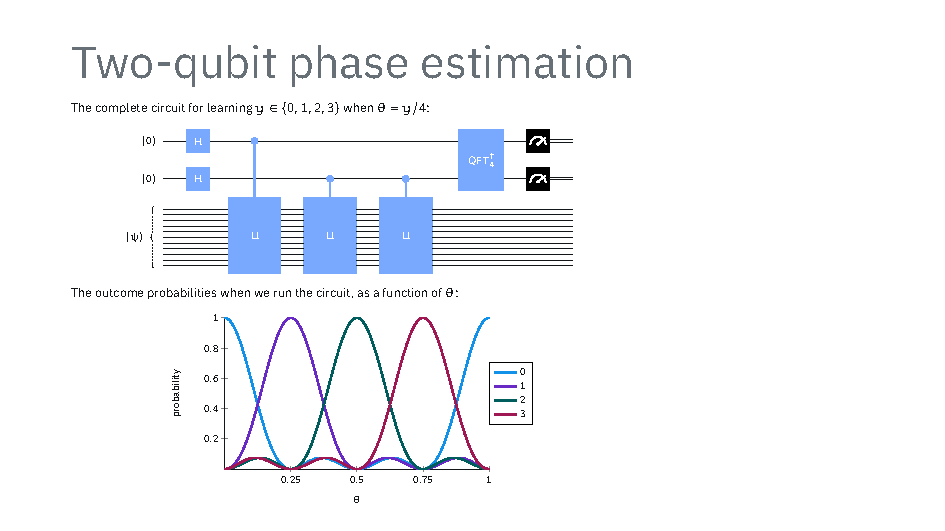
\includegraphics[height=3.4cm, trim={2.9cm 0.4cm 6.9cm 5.2cm}, clip]{phase-lecture/18_Phase-estimation-lecture-slides}
		\caption{2-qubit estimation}
		\label{fig:image1}
	\end{subfigure}
	
	% Add some vertical spacing between subfigures if desired
	\vspace{1ex} % Adjust the space as needed
	
	\begin{subfigure}[b]{\linewidth}
		\centering
		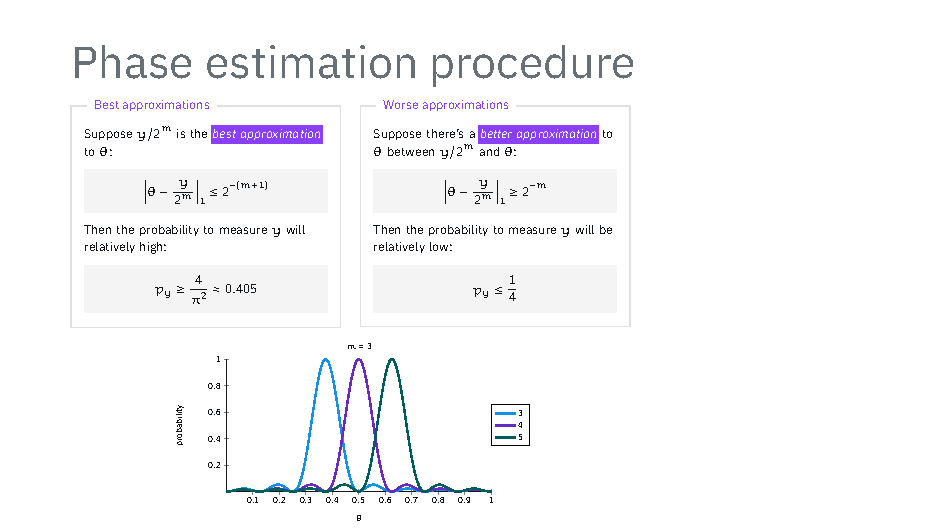
\includegraphics[height=3.4cm, trim={2.9cm 0.15cm 6.9cm 5.95cm}, clip]{phase-lecture/27_Phase-estimation-lecture-slides}
		\caption{3-qubit estimation}
		\label{fig:image2}
	\end{subfigure}
	
	\vspace{1ex} % Adjust the space as needed
	
	\begin{subfigure}[b]{\linewidth}
		\centering
		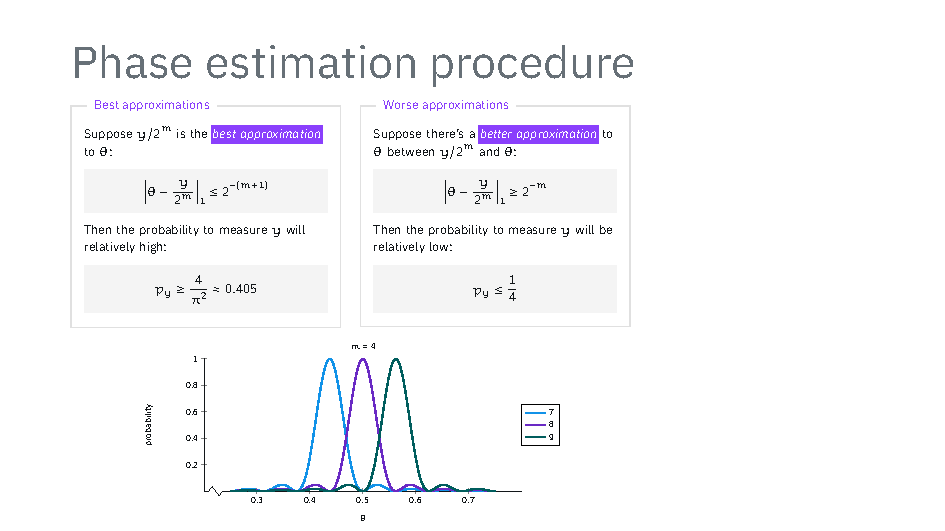
\includegraphics[height=3.4cm, trim={2.4cm 0.15cm 6.4cm 5.95cm}, clip]{phase-lecture/28_Phase-estimation-lecture-slides}
		\caption{4-qubit estimation}
		\label{fig:image3}
	\end{subfigure}
	
	\vspace{1ex} % Adjust the space as needed
	
	\begin{subfigure}[b]{\linewidth}
		\centering
		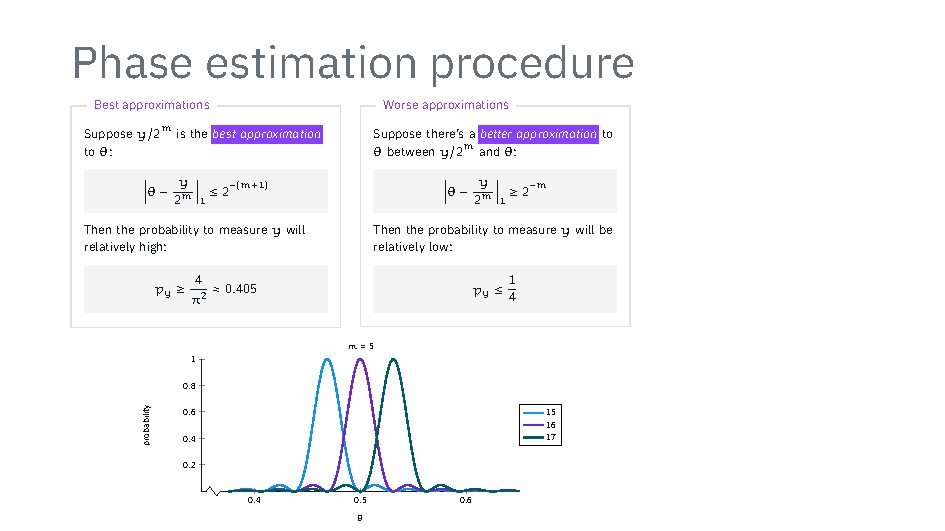
\includegraphics[height=3.4cm, trim={2.4cm 0.15cm 6.4cm 5.95cm}, clip]{phase-lecture/29_Phase-estimation-lecture-slides}
		\caption{5-qubit estimation}
		\label{fig:image4}
	\end{subfigure}
	
	\caption{Varying degree of precision by the phase estimation algorithm \cite{Phase-estimation}.}
	\label{fig:phase-precision}
\end{figure}
	
	%A simple example of minimizing the bottleneck travelling salesman problem (maybe with images):
	%an example of storing phases and using phase estimation
	%grover's search explanation
	\chapter{Algorithm}
	
The decision problem of the BTSP asks whether there exists a Hamiltonian cycle in which the weight of every edge is less than a specified threshold $\alpha$. In such a cycle, if we denote the weight of any edge as $\gamma_i$, then it must satisfy the condition:
	
	\begin{equation}\label{constraint-alpha} 
	 \gamma_i < \alpha
	\end{equation}
	
	We will construct the algorithm in the following steps:
	\begin{enumerate}
		\item Normalize edge weights so no single hamiltonian cycle is greater than or equal to 1. This is to ensure we can appropriately use the phase estimation algorithm.\\
		\item Construct a unitary operator that holds information regarding the hamiltonian cyles as phases in the diagonal. Our approach aligns with the findings presented by Ramakrishnan, Sharma, and Punnen: \cite{srinivasan2018efficient}\\
		\item Set all edgeweights $\geq \alpha$ to zero and construct a secondary unitary operator similiar to step 2.\\
		\item Create controlled gates using the unitary operators constructed in Step 2 and 3.\\
		\item Identify all the eigenstates of the unitary operators that map to the phases associated with the hamiltonian cycles.\\
		\item Perform phase estimation twice with an eigenstate using the control gates to evaluate the hamiltonian cycle before and after the edgeweights $\geq \alpha$ are set to zero.\\
		\item Compare the two phases achieved. If they are equal, the corresponding hamiltonian cycle is a solution that satisfies the constraint.\\
		
	\end{enumerate}
		
	\section{Normalize Edge Weights}
	
	A hamiltonian cycle of a complete graph with $N$ nodes requires $N$ edge-weights to complete the cycle. A single graph consists a total of $N(N-1)$ edgeweights in a directed graph. we can choose the largest $N$ and use these to normalize the edge weights. Let $w$ describe our edge-weights and will be a list of $m = N(N-1)$ elements:
	
	$$w = \{w_1, w_2, \ldots, w_m\}$$ 
	
	Sort $w$ in descending order to obtain:
	
	\begin{equation}\label{sorted-weights}
	w' = \{w'_1, w'_2, \ldots, w'_m\}
	\end{equation}
	
	Where: \begin{itemize}
		\item[] $w'_1 \geq w'_2 \geq \ldots \geq w'_m$
		\end{itemize}
		
The sum $S$ of the largest $N$ items in $w$ can be described as:

\begin{equation}\label{sum-S}
S = \sum_{i=1}^{N} w'_i
\end{equation}

  We can now perform the normalization. Let $\tilde{w}$ describe our normalized edge-weights:
  
 \begin{equation}\label{normalization}
  	\tilde{w} = (S + \epsilon)^{-1}w
\end{equation}

		Where: $\epsilon>0$.  The purpose of $\epsilon$ is to make sure if any normalized hamiltonian cycle is exactly equal to $ S$ then we do not have a zero phase.
	
	
	\section{Unitary Operator and Eigenstates associated with the Hamiltonian Cycles}
	
	 We start by constructing diagonal matrices $U_j$, one for each node in a complete graph and describe the matrix elements:
	
	\begin{equation}\label{Uj-elements}
	\left[U_j \right]_{kk} = e^{2\pi i\gamma_{jk} (1 - \delta_{jk})}
	\end{equation}
	
	Where:	\begin{itemize}
		\item[]  $ 1 \leq j, k \leq N$
		\item[]  $N$ denotes the total number of nodes.
		\item[]  $\gamma_{jk}$ represents the edgeweight connecting node $j\rightarrow k$.
	\end{itemize}
	
	
	Then we construct $U$, a tensor product of all the diagonal matrices:
	\begin{equation}\label{U-tensor}
	 U = \bigotimes_j^N U_j
	 \end{equation}
	
	
	$U$ will be a $N^N \times N^N$ matrix with only the diagonal elements populated. Because the diagonal elements will entirely consist of phases $\left[U \right]_{kk} = e^{i\alpha_{kk}} $. We can confirm the unitary operator condition is satisfied: $U^\dagger U = \mathds{1}$. 
	
	
	Given $U$'s diagonal nature, its eigenstates align with the basis vectors. Our focus is on specific eigenstates corresponding to the Hamiltonian cycles, determined by the phases. To comprehend how the diagonal elements of $U$ derive from the individual $U_j$ matrices, we visualize the tensor product construction. Notably, the product populates the diagonal elements of $U$ allowing a simplification where we consider these elements directly:
	
	\begin{flalign*}
	[U]_{0} & = [U_1]_{0}\cdot [U_2] _{0}\cdot \ldots  \cdot [U_{N-2}]_{0} \cdot [U_{N-1}]_{0}\cdot [U_N]_{0} \\
	[U]_{1}  & = [U_1]_{0}\cdot [U_2] _{0}\cdot \ldots \cdot [U_{N-2}]_{0}\cdot [U_{N-1}]_{0}\cdot [U_N]_{1}\\
	&  \vdots\\
	[U]_{N-1} &= [U_1]_{0}\cdot [U_2] _{0}\cdot \ldots\cdot [U_{N-2}]_{0} \cdot [U_{N-1}]_{0}\cdot [U_N]_{N-1}\\
	[U]_{N} &= [U_1]_{0}\cdot [U_2] _{0}\cdot \ldots \cdot [U_{N-2}]_{0} \cdot [U_{N-1}]_{1}\cdot [U_N]_{0}\\
	& \vdots\\
	[U]_{2N - 1} & = [U_1]_{0}\cdot [U_2] _{0}\cdot \ldots \cdot [U_{N-2}]_{0} \cdot [U_{N-1}]_{1}\cdot [U_N]_{N-1}\\
	[U]_{2N} &= [U_1]_{0}\cdot [U_2] _{0}\cdot \ldots \cdot [U_{N-2}]_{0} \cdot [U_{N-1}]_{2}\cdot [U_N]_{0}\\
	& \vdots\\
	[U]_{N^2 - 1 } & = [U_1]_{0}\cdot [U_2] _{0}\cdot \ldots \cdot [U_{N-2}]_{0} \cdot [U_{0}]_{N-1}\cdot [U_N]_{N-1}\\
	[U]_{N^2} &= [U_1]_{0}\cdot [U_2] _{0}\cdot \ldots \cdot [U_{N-2}]_{1} \cdot [U_{N-1}]_{0}\cdot [U_N]_{0}\\
	& \vdots\\
	[U]_{N^2 + N - 1} & = [U_1]_{0}\cdot [U_2] _{0}\cdot \ldots \cdot [U_{N-2}]_{1} \cdot [U_{N-1}]_{0}\cdot [U_N]_{N-1}\\
	[U]_{N^2 + N } &= [U_1]_{0}\cdot [U_2] _{0}\cdot \ldots \cdot [U_{N-2}]_{1} \cdot [U_{N-1}]_{1}\cdot [U_N]_{0}\\
	&  \vdots\\
	[U]_{N^3- 1} & = [U_1]_{0}\cdot [U_2] _{0}\cdot \ldots \cdot [U_{N-2}]_{N-1} \cdot [U_{N-1}]_{N-1}\cdot [U_N]_{N-1}
	\end{flalign*}
	This pattern indicates:
	\begin{equation}\label{U-matrix-eq}
	[U]_{k} = [U_1]_{\alpha_{N-1}}\cdot [U_2] _{\alpha_{N-2}}\cdot \ldots \cdot [U_{N-2}]_{\alpha_2} \cdot [U_{2}]_{\alpha_{1}}\cdot [U_N]_{\alpha_{0}}
	\end{equation}
	
	Where: \begin{itemize}
		\item[] $$\alpha_i = \left(k//\left(N^{i}\right)\right) \% N$$
		\item[] $//$ denotes integer division
	    \item[] $\%$ is the modulus operation
	    \end{itemize}
	
 	We can see the pattern follows base-$N$ counting where $N$ is the total number of nodes. Simply converting $k$ into base-$N$, will give us the indices of our original diagonal matrices. To locate the relevent eigenstates, we start by identifying the elements in $U_j$ associated  with a hamiltonian cycle, retrieve their respective indices, convert this string of indices from Base-$N$ to $k$.  and we would have identified our eigenstate $|k\rangle$. 
	
	\subsection{The Four City Graph}
	
	
	\begin{center}	
	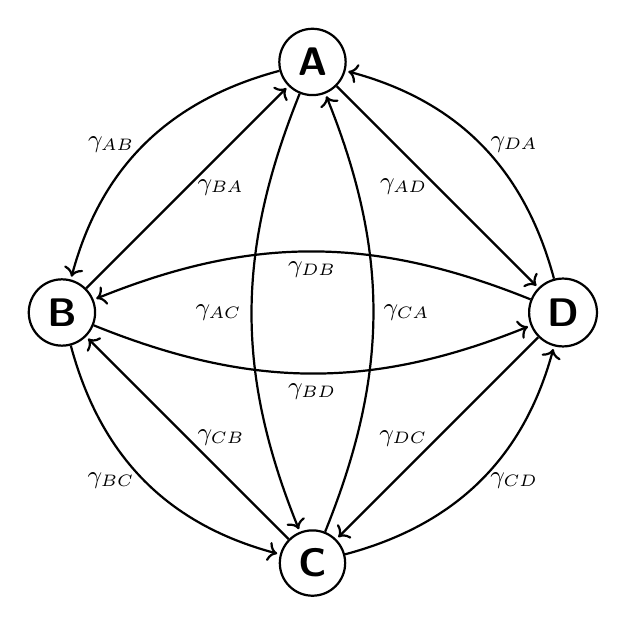
\begin{tikzpicture}[->,shorten >=1pt,auto,node distance=4.5cm, thick,main node/.style={circle,draw,font=\sffamily\Large\bfseries}]
		
		\node[main node] (1) {A};
		\node[main node] (2) [below left of=1] {B};
		\node[main node] (3) [below right of=2] {C};
		\node[main node] (4) [below right of=1] {D};
		
		\path[every node/.style={font=\sffamily\small}]
		(1) edge node [left] {$\gamma_{AD}$} (4)
		edge [bend right] node[left] {$\gamma_{AB}$} (2)
		edge[bend right=22] node[left] {$\gamma_{AC}$} (3)
		%edge [loop above] node {0.1} (1)
		(2) edge node [right] {$\gamma_{BA}$} (1)
		edge[bend right=22] node[below] {$\gamma_{BD}$} (4)
		%edge [loop left] node {0.4} (2)
		edge [bend right] node[left] {$\gamma_{BC}$} (3)
		(3) edge node [right] {$\gamma_{CB}$} (2)
		edge [bend right] node[right] {$\gamma_{CD}$} (4)
		edge[bend right=22] node[right] {$\gamma_{CA}$} (1)
		(4) edge node [left] {$\gamma_{DC}$} (3)
		%edge [loop right] node {0.6} (4)
		edge[bend right=22] node {$\gamma_{DB}$} (2)
		edge [bend right] node[right] {$\gamma_{DA}$} (1);
	\end{tikzpicture}
	
	\end{center}
	
	
	
	For the 4 city problem we will start with four matrices to represent the $12$ edgeweights from each node. Using \ref{Uj-elements}, Where:	$ j, k \in \{A,B,C,D\}$.  we can construct matrix $A$:

	$$
	A = \begin{bmatrix}
		1 & 0 & 0 & 0 \\
		0 & e^{i2\pi\gamma_{AB}} & 0 & 0 \\
		0 & 0 & e^{i2\pi\gamma_{AC}} & 0 \\
		0 & 0 & 0 & e^{i2\pi\gamma_{AD}} \\
	\end{bmatrix}
	$$
	
	Since we only populate the diagonal elements, we can ignore the other elements of the matrix. Let $ a = \mathrm{diag}(A)$, and lets construct the other diagonals:
	
	\begin{align*}	
		a & = \begin{bmatrix}
			1 \\
			e^{i2\pi\gamma_{AB}} \\
			e^{i2\pi\gamma_{AC}} \\
			e^{i2\pi\gamma_{AD}} \\
		\end{bmatrix} 
		b  = \begin{bmatrix}
			e^{i2\pi\gamma_{BA}} \\
			1 \\
			e^{i2\pi\gamma_{BC}} \\
			e^{i2\pi\gamma_{BD}} \\
		\end{bmatrix}
		c  = \begin{bmatrix}
			e^{i2\pi\gamma_{CA}} \\
			e^{i2\pi\gamma_{CB}} \\
			1 \\
			e^{i2\pi\gamma_{CD}} \\
		\end{bmatrix} 
		d = \begin{bmatrix}
			e^{i2\pi\gamma_{DA}} \\
			e^{i2\pi\gamma_{DB}} \\
			e^{i2\pi\gamma_{DC}} \\
			1 \\
		\end{bmatrix} 						 			
	\end{align*}
	
	
	We then construct the tensor product with equation \ref{U-tensor}:
	
	\begin{equation}\label{4-city-matrix-tensor}
	 U = A \otimes B \otimes C \otimes D
	\end{equation}
	
	The convience of dealing with only the diagonals we can similiarly state $ u = \mathrm{diag}(U)$, thus:
	
	$$ u = a \otimes b \otimes c \otimes d$$
	
	
	Refering to equation \ref{U-matrix-eq} regarding the matrix elements for U,  the diagonal elements for the 4-city problem will reduce to:
	
	\begin{equation}\label{4-city-tensor}
		u_{k} = a_{\alpha_{3}}\cdot b _{\alpha_{2}} \cdot c_{\alpha_1} \cdot d_{\alpha_{0}}
	\end{equation}
	
	With: $$\alpha_i = \left(k//\left(4^{i}\right)\right) \% 4$$
	
	
	\vspace{0.5cm}
	
	lets walk through identifying the eigenstate of one hamiltonian cycle. Lets say the cycle we choose is the following:
	
	\begin{equation}\label{one-ham-cycle-4-city}
		A \rightarrow D \rightarrow B \rightarrow C \rightarrow A
	\end{equation}
	from here we can identify the edgeweights we care about are:
	
	\begin{equation*}
		\gamma_{AD} + \gamma_{DB} + \gamma_{BC} + \gamma_{CA}
	\end{equation*}
	
	Thus the phase we would like to estimate would be given by the following element product:
	
	\begin{equation*}
		\Large{a_{3} \cdot d_{1} \cdot b_{2} \cdot c_{0} = e^{i2\pi (\gamma_{AD} + \gamma_{DB} + \gamma_{BC} + \gamma_{CA})}}
	\end{equation*}
	
	
	To correctly identify the eigenstate, we need to rearrange the product to match the form of equation \ref{4-city-tensor}:
	
	\begin{equation*}
		\Large{a_{3} \cdot d_{1} \cdot b_{2} \cdot c_{0} = \Large{a_{3}} \cdot b_{2} \cdot c_{0}  \cdot d_{1}}
	\end{equation*}
	
	From here we simply read out the indices and based on our discussion under equation \ref{U-matrix-eq} , we can infer we are working in base 4. Thus we simply need to convert to base 10 to understand the exact column number and to base 2 to be used as the initialized eigenstate.
	
	\begin{equation*}
		\text{base } 4 = 3201 \leftrightarrow \text{base } 10 = 225 \leftrightarrow  \text{base } 2 = 11100001
	\end{equation*}
	
	Thus our eigenstate for \ref{one-ham-cycle-4-city} will be  $|225\rangle$ or $|11100001\rangle$. We can perform an identical process for all the hamiltonian cycles to find their corresponding eigenstates. These are all listed in table \ref{table:ham-cycle-details-4-city} and and \ref{table:4-city-conversions}
	
	
	\begin{table}[h]
		\centering
		\begin{tabular}{|c|c|c|}
			\hline
			\textbf{Hamiltonian Cycle} & \textbf{Edge Weights Sum} & \textbf{Diagonal Elements Product} \\
			\hline
			$A \rightarrow B \rightarrow C \rightarrow D \rightarrow A$ & $\gamma_{AB} + \gamma_{BC} + \gamma_{CD} + \gamma_{DA}$ & $a_{1} \cdot b_{2} \cdot c_{3} \cdot d_{0}$ \\
			$A \rightarrow B \rightarrow D \rightarrow C \rightarrow A$ & $\gamma_{AB} + \gamma_{BD} + \gamma_{DC} + \gamma_{CA}$ & $a_{1} \cdot b_{3} \cdot d_{2} \cdot c_{0}$ \\
			$A \rightarrow C \rightarrow B \rightarrow D \rightarrow A$ & $\gamma_{AC} + \gamma_{CB} + \gamma_{BD} + \gamma_{DA}$ & $a_{2} \cdot c_{1} \cdot b_{3} \cdot d_{0}$ \\
			$A \rightarrow C \rightarrow D \rightarrow B \rightarrow A$ & $\gamma_{AC} + \gamma_{CD} + \gamma_{DB} + \gamma_{BA}$ & $a_{2} \cdot c_{3} \cdot d_{1} \cdot b_{0}$ \\
			$A \rightarrow D \rightarrow B \rightarrow C \rightarrow A$ & $\gamma_{AD} + \gamma_{DB} + \gamma_{BC} + \gamma_{CA}$ & $a_{3} \cdot d_{1} \cdot b_{2} \cdot c_{0}$ \\
			$A \rightarrow D \rightarrow C \rightarrow B \rightarrow A$ & $\gamma_{AD} + \gamma_{DC} + \gamma_{CB} + \gamma_{BA}$ & $a_{3} \cdot d_{2} \cdot c_{1} \cdot b_{0}$ \\
			\hline
			\end{tabular}
					\caption{Hamiltonian cycles of the directed 4-city graph with their edgeweight summation and expected diagonal element products (\ref{4-city-tensor}).}
			\label{table:ham-cycle-details-4-city}
	\end{table}
	\begin{table}[h]
		\centering
		\begin{tabular}{|c|c|c|}	
			
			\hline
			\textbf{Rearranged Indices (Base 4)} & \textbf{Base 10} & \textbf{Base 2} \\
			\hline
			1230 & 108 & 01101100 \\
			1302 & 114 & 01110010 \\
			2310 & 180 & 10110100 \\
			2031 & 141 & 10001101 \\
			3201 & 225 & 11100001 \\
			3012 & 198 & 11000110 \\
			\hline
		\end{tabular}
		\caption{Eigenstates of matrix $U$ (\ref{4-city-matrix-tensor}), containing the normalized hamiltonian cycle edge weight sum of the directed 4-city graph.}
		\label{table:4-city-conversions}
	\end{table}
	
	\subsection{The Five City Graph}
	
	
	
		\begin{center}	
		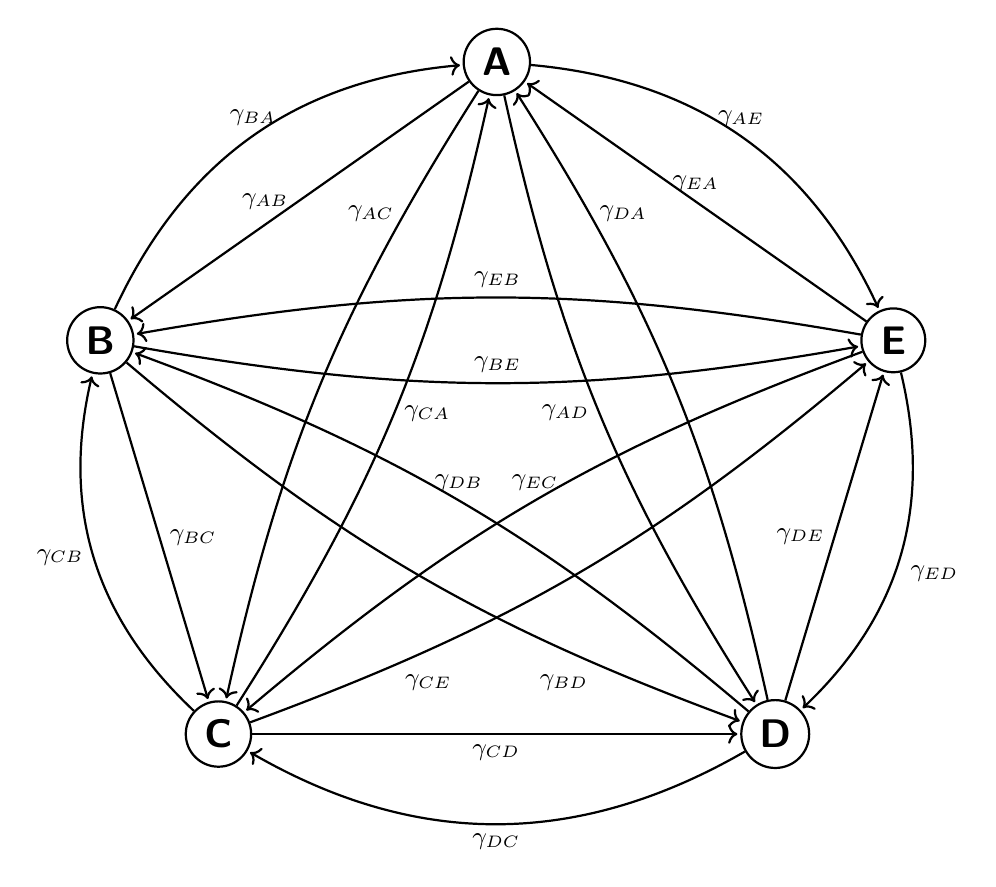
\begin{tikzpicture}[->,shorten >=1pt,auto,node distance=5cm, thick,main node/.style={circle,draw,font=\sffamily\Large\bfseries}]
			
			\node[main node] (1) {A};
			\node[main node] (2) [below left of=1, xshift = -1.5cm] {B};
			\node[main node] (3) [below of=2, xshift= 1.5cm] {C};
			\node[main node] (5) [below right of=1, xshift = 1.5cm] {E};
			\node[main node] (4) [below of=5, xshift= -1.5cm] {D};
			
			\path[every node/.style={font=\sffamily\small}]
			(1) edge [bend right=10] node [left] {$\gamma_{AD}$} (4)
			edge node[left] {$\gamma_{AB}$} (2)
			edge [bend right=10] node[left, pos = 0.2] {$\gamma_{AC}$} (3)
			edge[bend left] node[above] {$\gamma_{AE}$} (5)

			(2) edge[bend left] node [above] {$\gamma_{BA}$} (1)
			edge [bend right=10]  node[below left , pos = 0.8] {$\gamma_{BD}$} (4)
			edge node[right] {$\gamma_{BC}$} (3)
			edge [bend right=10] node[above] {$\gamma_{BE}$} (5)
			
			(3) edge[bend left] node [left] {$\gamma_{CB}$} (2)
			edge node[below] {$\gamma_{CD}$} (4)
			edge [bend right=10] node[right] {$\gamma_{CA}$} (1)
			edge [bend right=10] node[below right , pos = 0.2] {$\gamma_{CE}$} (5)
			
			(4) edge[bend left] node[below] {$\gamma_{DC}$} (3)
			edge [bend right=10] node[above] {$\gamma_{DB}$} (2)
			edge [bend right=10] node[right, pos = 0.8] {$\gamma_{DA}$} (1)
			edge node[left] {$\gamma_{DE}$} (5)
			
			(5) edge node [above] {$\gamma_{EA}$} (1)
			edge [bend right=10]  node[above] {$\gamma_{EB}$} (2)
			edge [bend right=10] node[above] {$\gamma_{EC}$} (3)
			edge[bend left] node {$\gamma_{ED}$} (4);

		\end{tikzpicture}
		
	\end{center}
	
	
	We construct our matrix U with the tensor product as in equation \ref{U-tensor}.
	
	\begin{equation}\label{5-city-matrix-tensor}
		U = A \otimes B \otimes C \otimes D \otimes E
	\end{equation}
	
	 Similiar to the four-city graph we only populate the diagonal elements, Let $ a = \mathrm{diag}(A)$, and let us construct the other diagonals:
	
	\begin{align*}	
		a & = \begin{bmatrix}
			1 \\
			e^{i2\pi\gamma_{AB}} \\
			e^{i2\pi\gamma_{AC}} \\
			e^{i2\pi\gamma_{AD}} \\
			e^{i2\pi\gamma_{AE}} \\
		\end{bmatrix} 
		b  = \begin{bmatrix}
			e^{i2\pi\gamma_{BA}} \\
			1 \\
			e^{i2\pi\gamma_{BC}} \\
			e^{i2\pi\gamma_{BD}} \\
			e^{i2\pi\gamma_{BE}} \\
		\end{bmatrix}
		c  = \begin{bmatrix}
			e^{i2\pi\gamma_{CA}} \\
			e^{i2\pi\gamma_{CB}} \\
			1 \\
			e^{i2\pi\gamma_{CD}} \\
			e^{i2\pi\gamma_{CE}} \\
		\end{bmatrix} 
		d = \begin{bmatrix}
			e^{i2\pi\gamma_{DA}} \\
			e^{i2\pi\gamma_{DB}} \\
			e^{i2\pi\gamma_{DC}} \\
			1 \\
			e^{i2\pi\gamma_{DE}} \\
		\end{bmatrix}  
		e = \begin{bmatrix}
			e^{i2\pi\gamma_{EA}} \\
			e^{i2\pi\gamma_{EB}} \\
			e^{i2\pi\gamma_{EC}} \\
			e^{i2\pi\gamma_{ED}} \\
			1 \\
		\end{bmatrix}		 			
	\end{align*}
	

	
	We can state $ u = \mathrm{diag}(U)$, thus:
	
	$$ u = a \otimes b \otimes c \otimes d \otimes e$$
	
	
	Refering to equation \ref{U-matrix-eq} regarding the matrix elements for U,  the diagonal elements for the 5-city problem will reduce to:
	
	\begin{equation}\label{5-city-tensor}
		u_{k} = a_{\alpha_{4}}\cdot b _{\alpha_{3}} \cdot c_{\alpha_2} \cdot d_{\alpha_{1}}\cdot e_{\alpha_{0}}
	\end{equation}
	
	With: $$\alpha_i = \left(k//\left(5^{i}\right)\right) \% 5$$
	
	
	\vspace{0.5cm}
	
	Let us walk through identifying the eigenstate of one hamiltonian cycle:
	
	\begin{equation}\label{one-ham-cycle-4-city}
		A \rightarrow E \rightarrow D \rightarrow C \rightarrow B \rightarrow A
	\end{equation}
	
	from here we can identify the edgeweights we care about are:
	
	\begin{equation*}
		\gamma_{AE} + \gamma_{ED} + \gamma_{DC} + \gamma_{CB} + \gamma_{BA}
	\end{equation*}
	
	Thus the phase we would like to estimate would be given by the following element product:
	
	\begin{equation*}
		\Large{a_{4} \cdot e_{3} \cdot d_{2} \cdot c_{1} \cdot b_{0} = e^{i2\pi (\gamma_{AE} + \gamma_{ED} + \gamma_{DC} + \gamma_{CB} + \gamma_{BA})}}
	\end{equation*}
	
	
	To correctly identify the eigenstate, we need to rearrange the product to match the form of equation \ref{5-city-tensor}:
	
	\begin{equation*}
		\Large{a_{4} \cdot e_{3} \cdot d_{2} \cdot c_{1} \cdot b_{0}= a_{4} \cdot b_{0}  \cdot c_{1}\cdot d_{2} \cdot e_{3}}
	\end{equation*}
	
	From here we simply read out the indices and based on our discussion under equation \ref{U-matrix-eq} , we can infer we are working in base 4. Thus we simply need to convert to base 10 to understand the exact column number and to base 2 to be used as the initialized eigenstate.
	
	\begin{equation*}
		\text{base } 5 = 40123 \leftrightarrow \text{base } 10 = 2538 \leftrightarrow  \text{base } 2 = 100111101010
	\end{equation*}
	
	Thus our eigenstate for \ref{one-ham-cycle-4-city} will be  $|2538\rangle$ or $|100111101010\rangle$. We can perform an identical process for all the hamiltonian cycles to find their corresponding eigenstates. These are all listed in table \ref{table:ham-cycle-details-5-city} and \ref{table:5-city-conversions}
	
	
	
	
	\begin{table}[h]
		\centering
		\begin{tabular}{|c|c|c|}
			\hline
			\textbf{Hamiltonian Cycle} & \textbf{Edge Weights Sum} & \textbf{Matrix Elements Product} \\
			\hline
$A \rightarrow B \rightarrow C \rightarrow D \rightarrow E \rightarrow A$ & $ \gamma_{AB} + \gamma_{BC} + \gamma_{CD} + \gamma_{DE} + \gamma_{EA}$ & $a_1  \cdot b_2 \cdot c_3 \cdot d_4 \cdot e_0$ \\
$A \rightarrow B \rightarrow C \rightarrow E \rightarrow D \rightarrow A$ & $ \gamma_{AB} + \gamma_{BC} + \gamma_{CE} + \gamma_{ED} + \gamma_{DA}$ & $a_1  \cdot b_2 \cdot c_4 \cdot e_3 \cdot d_0$ \\
$A \rightarrow B \rightarrow D \rightarrow C \rightarrow E \rightarrow A$ & $ \gamma_{AB} + \gamma_{BD} + \gamma_{DC} + \gamma_{CE} + \gamma_{EA}$ & $a_1  \cdot b_3 \cdot d_2 \cdot c_4 \cdot e_0$ \\
$A \rightarrow B \rightarrow D \rightarrow E \rightarrow C \rightarrow A$ & $ \gamma_{AB} + \gamma_{BD} + \gamma_{DE} + \gamma_{EC} + \gamma_{CA}$ & $a_1  \cdot b_3 \cdot d_4 \cdot e_2 \cdot c_0$ \\
$A \rightarrow B \rightarrow E \rightarrow C \rightarrow D \rightarrow A$ & $ \gamma_{AB} + \gamma_{BE} + \gamma_{EC} + \gamma_{CD} + \gamma_{DA}$ & $a_1  \cdot b_4 \cdot e_2 \cdot c_3 \cdot d_0$ \\
$A \rightarrow B \rightarrow E \rightarrow D \rightarrow C \rightarrow A$ & $ \gamma_{AB} + \gamma_{BE} + \gamma_{ED} + \gamma_{DC} + \gamma_{CA}$ & $a_1  \cdot b_4 \cdot e_3 \cdot d_2 \cdot c_0$ \\
$A \rightarrow C \rightarrow B \rightarrow D \rightarrow E \rightarrow A$ & $ \gamma_{AC} + \gamma_{CB} + \gamma_{BD} + \gamma_{DE} + \gamma_{EA}$ & $a_2  \cdot c_1 \cdot b_3 \cdot d_4 \cdot e_0$ \\
$A \rightarrow C \rightarrow B \rightarrow E \rightarrow D \rightarrow A$ & $ \gamma_{AC} + \gamma_{CB} + \gamma_{BE} + \gamma_{ED} + \gamma_{DA}$ & $a_2  \cdot c_1 \cdot b_4 \cdot e_3 \cdot d_0$ \\
$A \rightarrow C \rightarrow D \rightarrow B \rightarrow E \rightarrow A$ & $ \gamma_{AC} + \gamma_{CD} + \gamma_{DB} + \gamma_{BE} + \gamma_{EA}$ & $a_2  \cdot c_3 \cdot d_1 \cdot b_4 \cdot e_0$ \\
$A \rightarrow C \rightarrow D \rightarrow E \rightarrow B \rightarrow A$ & $ \gamma_{AC} + \gamma_{CD} + \gamma_{DE} + \gamma_{EB} + \gamma_{BA}$ & $a_2  \cdot c_3 \cdot d_4 \cdot e_1 \cdot b_0$ \\
$A \rightarrow C \rightarrow E \rightarrow B \rightarrow D \rightarrow A$ & $ \gamma_{AC} + \gamma_{CE} + \gamma_{EB} + \gamma_{BD} + \gamma_{DA}$ & $a_2  \cdot c_4 \cdot e_1 \cdot b_3 \cdot d_0$ \\
$A \rightarrow C \rightarrow E \rightarrow D \rightarrow B \rightarrow A$ & $ \gamma_{AC} + \gamma_{CE} + \gamma_{ED} + \gamma_{DB} + \gamma_{BA}$ & $a_2  \cdot c_4 \cdot e_3 \cdot d_1 \cdot b_0$ \\
$A \rightarrow D \rightarrow B \rightarrow C \rightarrow E \rightarrow A$ & $ \gamma_{AD} + \gamma_{DB} + \gamma_{BC} + \gamma_{CE} + \gamma_{EA}$ & $a_3  \cdot d_1 \cdot b_2 \cdot c_4 \cdot e_0$ \\
$A \rightarrow D \rightarrow B \rightarrow E \rightarrow C \rightarrow A$ & $ \gamma_{AD} + \gamma_{DB} + \gamma_{BE} + \gamma_{EC} + \gamma_{CA}$ & $a_3  \cdot d_1 \cdot b_4 \cdot e_2 \cdot c_0$ \\
$A \rightarrow D \rightarrow C \rightarrow B \rightarrow E \rightarrow A$ & $ \gamma_{AD} + \gamma_{DC} + \gamma_{CB} + \gamma_{BE} + \gamma_{EA}$ & $a_3  \cdot d_2 \cdot c_1 \cdot b_4 \cdot e_0$ \\
$A \rightarrow D \rightarrow C \rightarrow E \rightarrow B \rightarrow A$ & $ \gamma_{AD} + \gamma_{DC} + \gamma_{CE} + \gamma_{EB} + \gamma_{BA}$ & $a_3  \cdot d_2 \cdot c_4 \cdot e_1 \cdot b_0$ \\
$A \rightarrow D \rightarrow E \rightarrow B \rightarrow C \rightarrow A$ & $ \gamma_{AD} + \gamma_{DE} + \gamma_{EB} + \gamma_{BC} + \gamma_{CA}$ & $a_3  \cdot d_4 \cdot e_1 \cdot b_2 \cdot c_0$ \\
$A \rightarrow D \rightarrow E \rightarrow C \rightarrow B \rightarrow A$ & $ \gamma_{AD} + \gamma_{DE} + \gamma_{EC} + \gamma_{CB} + \gamma_{BA}$ & $a_3  \cdot d_4 \cdot e_2 \cdot c_1 \cdot b_0$ \\
$A \rightarrow E \rightarrow B \rightarrow C \rightarrow D \rightarrow A$ & $ \gamma_{AE} + \gamma_{EB} + \gamma_{BC} + \gamma_{CD} + \gamma_{DA}$ & $a_4  \cdot e_1 \cdot b_2 \cdot c_3 \cdot d_0$ \\
$A \rightarrow E \rightarrow B \rightarrow D \rightarrow C \rightarrow A$ & $ \gamma_{AE} + \gamma_{EB} + \gamma_{BD} + \gamma_{DC} + \gamma_{CA}$ & $a_4  \cdot e_1 \cdot b_3 \cdot d_2 \cdot c_0$ \\
$A \rightarrow E \rightarrow C \rightarrow B \rightarrow D \rightarrow A$ & $ \gamma_{AE} + \gamma_{EC} + \gamma_{CB} + \gamma_{BD} + \gamma_{DA}$ & $a_4  \cdot e_2 \cdot c_1 \cdot b_3 \cdot d_0$ \\
$A \rightarrow E \rightarrow C \rightarrow D \rightarrow B \rightarrow A$ & $ \gamma_{AE} + \gamma_{EC} + \gamma_{CD} + \gamma_{DB} + \gamma_{BA}$ & $a_4  \cdot e_2 \cdot c_3 \cdot d_1 \cdot b_0$ \\
$A \rightarrow E \rightarrow D \rightarrow B \rightarrow C \rightarrow A$ & $ \gamma_{AE} + \gamma_{ED} + \gamma_{DB} + \gamma_{BC} + \gamma_{CA}$ & $a_4  \cdot e_3 \cdot d_1 \cdot b_2 \cdot c_0$ \\
$A \rightarrow E \rightarrow D \rightarrow C \rightarrow B \rightarrow A$ & $ \gamma_{AE} + \gamma_{ED} + \gamma_{DC} + \gamma_{CB} + \gamma_{BA}$ & $a_4  \cdot e_3 \cdot d_2 \cdot c_1 \cdot b_0$ \\
			\hline
			\end{tabular}
\caption{Hamiltonian cycles of the directed 4-city graph with their edgeweight summation and expected diagonal element products (\ref{5-city-tensor}).}
\label{table:ham-cycle-details-5-city}
\end{table}
\begin{table}[h]
\centering
\begin{tabular}{|c|c|c|}	
		
		\hline
		\textbf{Rearranged Indices (Base 5)} & \textbf{Base 10} & \textbf{Base 2} \\
		\hline
		12340 & 970 & 001111001010 \\
		12403 & 978 & 001111010010 \\
		13420 & 1110 & 010001010110 \\
		13042 & 1022 & 001111111110 \\
		14302 & 1202 & 010010110010 \\
		14023 & 1138 & 010001110010 \\
		23140 & 1670 & 011010000110 \\
		24103 & 1778 & 011011110010 \\
		24310 & 1830 & 011100100110 \\
		20341 & 1346 & 010101000010 \\
		23401 & 1726 & 011010111110 \\
		20413 & 1358 & 010101001110 \\
		32410 & 2230 & 100010110110 \\
		34012 & 2382 & 100101001110 \\
		34120 & 2410 & 100101101010 \\
		30421 & 1986 & 011111000010 \\
		32041 & 2146 & 100001100010 \\
		30142 & 1922 & 011110000010 \\
		42301 & 2826 & 101100001010 \\
		43021 & 2886 & 101101000110 \\
		43102 & 2902 & 101101010110 \\
		40312 & 2582 & 101000010110 \\
		42013 & 2758 & 101011000110 \\
		40123 & 2538 & 100111101010 \\
		\hline
		\end{tabular}
		\caption{Eigenstates of matrix $U$ (\ref{5-city-matrix-tensor}), containing the normalized hamiltonian cycle edge weight sum of the directed 4-city graph}
		\label{table:5-city-conversions}
	\end{table}
	
	


	
	\chapter{Simulations}
	

	
	\section{An Undirected 4-City Graph}
	
		Lets consider the following example of a symmetric 4-city system.  In this undirected graph we need to look at $(4-1)!/2 = 3$ hamiltonian cycles. The constraint for our BTSP in this case will involve $\gamma < 6$:
	\begin{center}	
		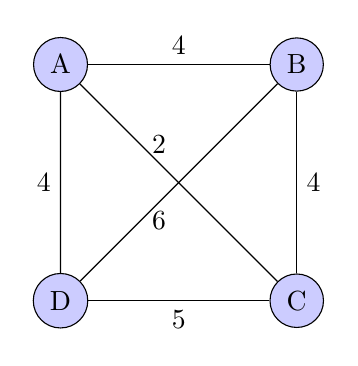
\begin{tikzpicture}[scale=3, every node/.style={circle, draw, fill=blue!20}]
			% Nodes
			\node (1) at (2,0) {D};
			\node (2) at (3,0) {C};
			\node (3) at (3,1) {B};
			\node (4) at (2,1) {A};
			% Edges with weights
			\draw (1) -- (2) node[midway, below, fill=none, draw=none, shape=rectangle] {5};
			\draw (2) -- (3) node[midway, right, fill=none, draw=none, shape=rectangle] {4};
			\draw (3) -- (4) node[midway, above, fill=none, draw=none, shape=rectangle] {4};
			\draw (4) -- (1) node[midway, left, fill=none, draw=none, shape=rectangle] {4};
			\draw (1) -- (3) node[pos = 0.4, below, fill=none, draw=none, shape=rectangle] {6};
			\draw (2) -- (4) node[pos = 0.6, above, fill=none, draw=none, shape=rectangle] {2};
		\end{tikzpicture}
	\end{center}
	
	\begin{equation*}
		w =  \{w_{AB},w_{AC},w_{AD},w_{BC},w_{CD},w_{BD}\} =  \{4,2,4,4,5,6\}
	\end{equation*}
	
	
	\subsection{Algorithm Construction}
	
	We will follow the instructions highlighted at the begining of chapter 3. We start by normalizing our edge weights. We need to sort our all edge weights in descending order as in equation \ref{sorted-weights}:	
	
	\begin{equation*}
	w' = \{6,5,4,4,4,2\}
	\end{equation*}
	
	
	Then we need to retrieve the sum $S$ as in equation \ref{sum-S}
	\begin{equation*}
	S = \sum_{i=1}^{4} w'_i = 6 + 5  + 4 + 4 = 19
	\end{equation*}
	
	From here we can normalize our edgeweights as in \ref{normalization}, we can set $\epsilon = 1$
	
	\begin{equation*}
		\tilde{w} = \frac{ \{4,2,4,4,5,6\}}{20} = \{0.2 , 0.1 , 0.2 , 0.2 , 0.25, 0.3\} 
	\end{equation*}
	
	
	
	
	\begin{center}	
		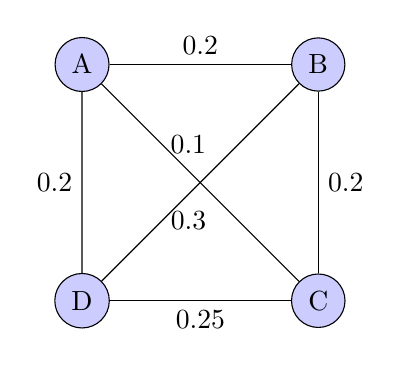
\begin{tikzpicture}[scale=3, every node/.style={circle, draw, fill=blue!20}]
			% Nodes
			\node (1) at (2,0) {D};
			\node (2) at (3,0) {C};
			\node (3) at (3,1) {B};
			\node (4) at (2,1) {A};
			% Edges with weights
			\draw (1) -- (2) node[midway, below, fill=none, draw=none, shape=rectangle] {0.25};
			\draw (2) -- (3) node[midway, right, fill=none, draw=none, shape=rectangle] {$0.2$};
			\draw (3) -- (4) node[midway, above, fill=none, draw=none, shape=rectangle] {$0.2$};
			\draw (4) -- (1) node[midway, left, fill=none, draw=none, shape=rectangle] {$0.2$};
			\draw (1) -- (3) node[pos = 0.4, below, xshift=1mm, fill=none, draw=none, shape=rectangle] {$0.3$};
			\draw (2) -- (4) node[pos = 0.6, above,xshift=1mm, fill=none, draw=none, shape=rectangle] {$0.1$};
		\end{tikzpicture}
	\end{center}
	
	
	Now we need to construct the unitary operator and eigenstates. Our matrix $U$ and $U'$ diagonals will look like the following:
	
	
	\begin{align*}	
		u & = \begin{bmatrix}
			1 \\
			e^{i2\pi(0.2)} \\
			e^{i2\pi(0.1)} \\
			e^{i2\pi(0.2)} \\
		\end{bmatrix} 
		\otimes \begin{bmatrix}
			e^{i2\pi(0.2)} \\
			1 \\
			e^{i2\pi(0.2)} \\
			e^{i2\pi(0.3)} \\
		\end{bmatrix}
		\otimes \begin{bmatrix}
			e^{i2\pi(0.1)} \\
			e^{i2\pi(0.2)} \\
			1\\
			e^{i2\pi(0.25)} \\
		\end{bmatrix} 
		\otimes \begin{bmatrix}
		e^{i2\pi(0.2)} \\
		e^{i2\pi(0.3)} \\
		e^{i2\pi(0.25)} \\
			1 \\
		\end{bmatrix} 						 			
	\end{align*}
	
	\begin{align*}	
		u' & = \begin{bmatrix}
			1 \\
			e^{i2\pi(0.2)} \\
			e^{i2\pi(0.1)} \\
			e^{i2\pi(0.2)} \\
		\end{bmatrix} 
		\otimes \begin{bmatrix}
			e^{i2\pi(0.2)} \\
			1 \\
			e^{i2\pi(0.2)} \\
			e^{i2\pi(0)} \\
		\end{bmatrix}
		\otimes \begin{bmatrix}
			e^{i2\pi(0.1)} \\
			e^{i2\pi(0.2)} \\
			1\\
			e^{i2\pi(0.25)} \\
		\end{bmatrix} 
		\otimes \begin{bmatrix}
			e^{i2\pi(0.2)} \\
			e^{i2\pi(0)} \\
			e^{i2\pi(0.25)} \\
			1 \\
		\end{bmatrix} 						 			
	\end{align*}
	
	To construct our controlled matrices we can use the block matrix structure shown in \ref{control-u-matrix}. the number of diagonal elements in $U$ and $U'$ is $4^4$ thus we need $8$ eigenstate qubits to represent all $256$ states:
	
	\begin{equation*}
		CU = \begin{bmatrix}
			\mathbb{I}_8 & 0 \\
			0 & U \\
		\end{bmatrix},\;\;\;
		CU' = \begin{bmatrix}
			\mathbb{I}_8 & 0 \\
			0 & U' \\
		\end{bmatrix}
	\end{equation*}
	
	
	Because we are dealing with the symmetric case. Based on Table \ref{table:ham-cycle-details-4-city} we can simply use the results and conversions from the first three cycles. Thus we will be estimating phases using the following eigenstates:
	
	$$|108\rangle = |01101100\rangle$$
	$$|114\rangle = |01110010\rangle$$
	$$|180\rangle = |10110100\rangle$$
	And expect the following phases:
	
	Cycle 1: $A \rightarrow B \rightarrow C \rightarrow D \rightarrow A$
	
	\begin{center}	
		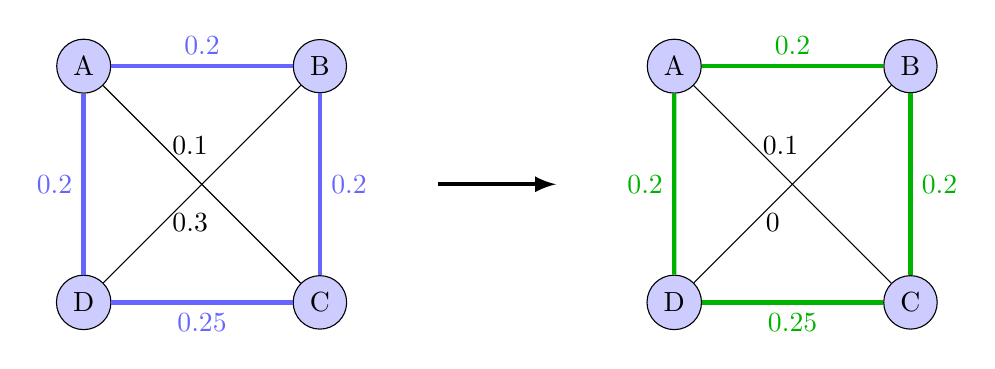
\begin{tikzpicture}[scale=3, every node/.style={circle, draw, fill=blue!20}]
			% Nodes
			\node (1) at (0,0) {D};
			\node (2) at (1,0) {C};
			\node (3) at (1,1) {B};
			\node (4) at (0,1) {A};
			% Edges with weights
			\draw[blue!60, ultra thick] (1) -- (2) node[midway, below, fill=none, draw=none, shape=rectangle] {$0.25$};
			\draw[blue!60,ultra  thick] (2) -- (3) node[midway, right, fill=none, draw=none, shape=rectangle] {$0.2$};
			\draw [blue!60, ultra thick](3) -- (4) node[midway, above, fill=none, draw=none, shape=rectangle] {$0.2$};
			\draw [blue!60,ultra  thick](4) -- (1) node[midway, left, fill=none, draw=none, shape=rectangle] {$0.2$};
			\draw (1) -- (3) node[pos = 0.4, xshift=1mm, below, fill=none, draw=none, shape=rectangle] {$0.3$};
			\draw (2) -- (4) node[pos = 0.6, xshift=1mm, above, fill=none, draw=none, shape=rectangle] {$0.1$};
			
			
			
			% Nodes
			\node (5) at (2.5,0) {D};
			\node (6) at (3.5,0) {C};
			\node (7) at (3.5,1) {B};
			\node (8) at (2.5,1) {A};
			% Edges with weights
			\draw[black!30!green, ultra thick] (5) -- (6) node[midway, below, fill=none, draw=none, shape=rectangle] {$0.25$};
			\draw[black!30!green, ultra thick] (6) -- (7) node[midway, right, fill=none, draw=none, shape=rectangle] {$0.2$};
			\draw [black!30!green, ultra thick](7) -- (8) node[midway, above, fill=none, draw=none, shape=rectangle] {$0.2$};
			\draw [black!30!green, ultra thick](8) -- (5) node[midway, left, fill=none, draw=none, shape=rectangle] {$0.2$};
			\draw (5) -- (7) node[pos = 0.4, below, fill=none, draw=none, shape=rectangle] {$0$};
			\draw (6) -- (8) node[pos = 0.6, xshift=1mm, above, fill=none, draw=none, shape=rectangle] {$0.1$};
			
			\draw[->, ultra thick, >=latex] (1.5, 0.5) -- (2, 0.5);
			
		\end{tikzpicture}
	\end{center}
	
	
	 $$u_{108} = e^{i2\pi (\gamma_{AB} + \gamma_{BC} + \gamma_{CD} + \gamma_{DA})} = e^{i2\pi(0.85)}$$
	 $$u'_{108} = e^{i2\pi (\gamma_{AB} + \gamma_{BC} + \gamma_{CD} + \gamma_{DA})} = e^{i2\pi(0.85)}$$
	 
	 
	 Cycle 2: $A \rightarrow B \rightarrow D \rightarrow C \rightarrow A$
	 
	 \begin{center}	
	 	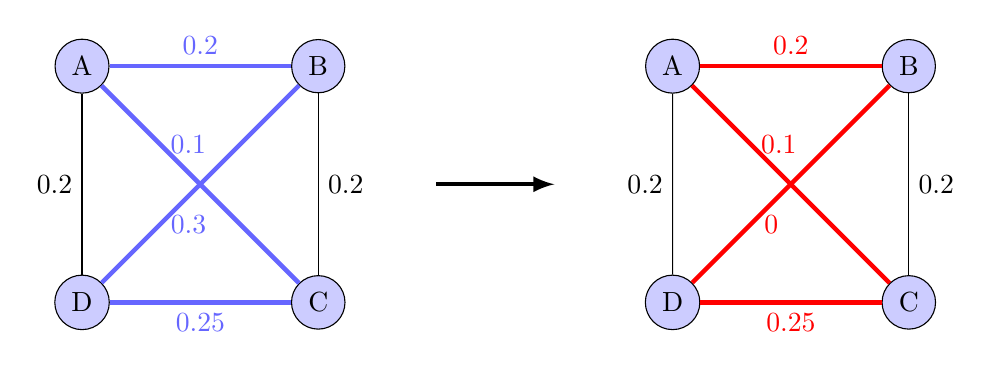
\begin{tikzpicture}[scale=3, every node/.style={circle, draw, fill=blue!20}]
	 		% Nodes
	 		\node (1) at (0,0) {D};
	 		\node (2) at (1,0) {C};
	 		\node (3) at (1,1) {B};
	 		\node (4) at (0,1) {A};
	 		% Edges with weights
	 		\draw [blue!60, ultra thick](1) -- (2) node[midway, below, fill=none, draw=none, shape=rectangle] {$0.25$};
	 		\draw (2) -- (3) node[midway, right, fill=none, draw=none, shape=rectangle] {$0.2$};
	 		\draw [blue!60, ultra thick](3) -- (4) node[midway, above, fill=none, draw=none, shape=rectangle] {$0.2$};
	 		\draw (4) -- (1) node[midway, left, fill=none, draw=none, shape=rectangle] {$0.2$};
	 		\draw [blue!60, ultra thick](1) -- (3) node[pos = 0.4, xshift=1mm, below, fill=none, draw=none, shape=rectangle] {$0.3$};
	 		\draw [blue!60, ultra thick](2) -- (4) node[pos = 0.6, xshift=1mm, above, fill=none, draw=none, shape=rectangle] {$0.1$};
	 		
	 		
	 		
	 		% Nodes
	 		\node (5) at (2.5,0) {D};
	 		\node (6) at (3.5,0) {C};
	 		\node (7) at (3.5,1) {B};
	 		\node (8) at (2.5,1) {A};
	 		% Edges with weights
	 		\draw[red, ultra thick] (5) -- (6) node[midway, below, fill=none, draw=none, shape=rectangle] {$0.25$};
	 		\draw (6) -- (7) node[midway, right, fill=none, draw=none, shape=rectangle] {$0.2$};
	 		\draw [red, ultra thick](7) -- (8) node[midway, above, fill=none, draw=none, shape=rectangle] {$0.2$};
	 		\draw (8) -- (5) node[midway, left, fill=none, draw=none, shape=rectangle] {$0.2$};
	 		\draw  [red, ultra thick](5) -- (7) node[pos = 0.4, below, fill=none, draw=none, shape=rectangle] {$0$};
	 		\draw  [red,ultra  thick](6) -- (8) node[pos = 0.6, xshift=1mm, above, fill=none, draw=none, shape=rectangle] {$0.1$};
	 		
	 		\draw[->, ultra thick, >=latex] (1.5, 0.5) -- (2, 0.5);
	 		
	 	\end{tikzpicture}
	 \end{center}
	 
	 $$ u_{114} = e^{i2\pi (\gamma_{AB} + \gamma_{BD} + \gamma_{DC} + \gamma_{CA})} = e^{i2\pi(0.85)}$$
	 $$ u'_{114} = e^{i2\pi (\gamma_{AB} + \gamma_{BD} + \gamma_{DC} + \gamma_{CA})} = e^{i2\pi(0.55)}$$
	 
	 
	 Cycle 3: $A \rightarrow C \rightarrow B \rightarrow D \rightarrow A$
	 
	 \begin{center}	
	 	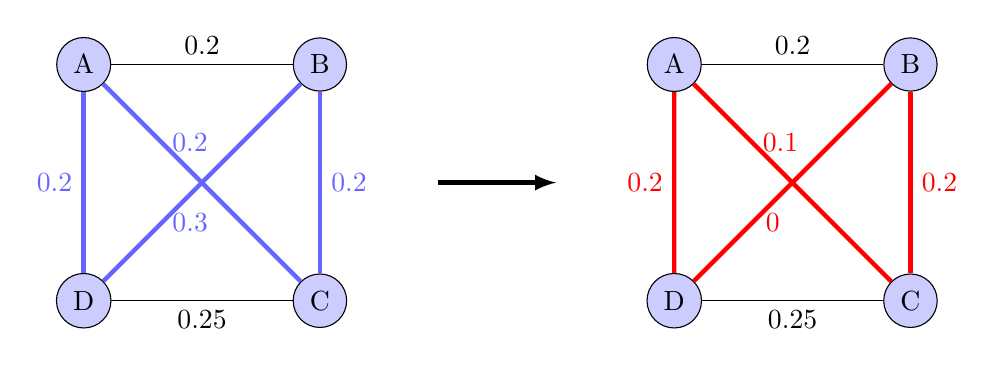
\begin{tikzpicture}[scale=3, every node/.style={circle, draw, fill=blue!20}]
	 		% Nodes
	 		\node (1) at (0,0) {D};
	 		\node (2) at (1,0) {C};
	 		\node (3) at (1,1) {B};
	 		\node (4) at (0,1) {A};
	 		% Edges with weights
	 		\draw (1) -- (2) node[midway, below, fill=none, draw=none, shape=rectangle] {$0.25$};
	 		\draw [blue!60, ultra thick](2) -- (3) node[midway, right, fill=none, draw=none, shape=rectangle] {$0.2$};
	 		\draw (3) -- (4) node[midway, above, fill=none, draw=none, shape=rectangle] {$0.2$};
	 		\draw [blue!60,ultra thick](4) -- (1) node[midway, left, fill=none, draw=none, shape=rectangle] {$0.2$};
	 		\draw [blue!60,ultra thick](1) -- (3) node[pos = 0.4, xshift=1mm, below, fill=none, draw=none, shape=rectangle] {$0.3$};
	 		\draw [blue!60,ultra thick](2) -- (4) node[pos = 0.6, xshift=1mm, above, fill=none, draw=none, shape=rectangle] {$0.2$};
	 		
	 		% Nodes
	 		\node (5) at (2.5,0) {D};
	 		\node (6) at (3.5,0) {C};
	 		\node (7) at (3.5,1) {B};
	 		\node (8) at (2.5,1) {A};
	 		% Edges with weights
	 		\draw (5) -- (6) node[midway, below, fill=none, draw=none, shape=rectangle] {$0.25$};
	 		\draw [red,ultra thick](6) -- (7) node[midway, right, fill=none, draw=none, shape=rectangle] {$0.2$};
	 		\draw (7) -- (8) node[midway, above, fill=none, draw=none, shape=rectangle] {$0.2$};
	 		\draw [red,ultra thick](8) -- (5) node[midway, left, fill=none, draw=none, shape=rectangle] {$0.2$};
	 		\draw  [red,ultra thick](5) -- (7) node[pos = 0.4, below, fill=none, draw=none, shape=rectangle] {$0$};
	 		\draw  [red,ultra thick](6) -- (8) node[pos = 0.6, xshift=1mm, above, fill=none, draw=none, shape=rectangle] {$0.1$};
	 		
	 		% Arrow pointing from the first graph to the second graph
	 		\draw[->, ultra thick, >=latex] (1.5, 0.5) -- (2, 0.5);% node[midway, above,  fill=none, draw=none, shape=rectangle] {Transition};
	 		
	 	\end{tikzpicture}
	 \end{center}
	 
	 $$ u_{180} = e^{i2\pi (\gamma_{AC} + \gamma_{CB} + \gamma_{BD} + \gamma_{DA})} = e^{i2\pi(0.80)}$$
	$$ u'_{180} = e^{i2\pi (\gamma_{AC} + \gamma_{CB} + \gamma_{BD} + \gamma_{DA})} = e^{i2\pi(0.50)}$$
	
	\subsection{Results: Simulations with Qiskit} \label{4-city-sim}
	
	We use Qiskit, an open source framework for quantum circuits to run simulations. Fig. \ref{fig:4-city-circuit} shows us the circuit for our first hamiltonian cycle initialized in eigenstate $|01101100\rangle$. We will run a similiar circuit for the other two hamiltonian cycles with the only change being the eigenstate initialization. We conduct an ideal simulation implying our results are not impacted by noise. Each circuit by default is run $1024$ times which we can use as a quasi-probability distribution. 
	


 \begin{figure}[!h]
		\centering
		\includegraphics[trim={8.5cm 4.4cm 6cm 4.4cm},clip, width=1 \linewidth]{"graphics/4-city-1-cycle-constrained-barrier"}
		\caption{the quantum circuit for the BTSP: 3 qubit phase estimation is performed measuring the hamiltonian cycle $A \rightarrow B \rightarrow C \rightarrow D \rightarrow A$, using the corresponding eigenstate is $|01101100\rangle$. Due to Qiskit convention on qubit ordering, the eigentate is initialized in reverse. The CU gate denotes the control unitary matrix containing all the hamiltonian cycles. The CU' gate inhabits the same cycles but before it was constructed, all edgeweights not satisfying the constraint, $\geq \alpha$, were set to zero. We have two sets of 3 qubits to be measured and stored in to classical registers labelled 'output' and 'output c'.}
		\label{fig:4-city-circuit}
	\end{figure}		


	\begin{figure}[!h]
		\centering
		\includegraphics[width=\textwidth,height=0.9\textheight,keepaspectratio]{"graphics/3qubit-4city"}
		\caption{3-qubit phase estimation for the 4-city graph}
		\label{fig:4-city-graphic-3}
	\end{figure}		
	
		\begin{figure}[!h]
		\centering
		\includegraphics[ width=\textwidth,height=0.9\textheight,keepaspectratio]{"graphics/4qubit-4city"}
		\caption{4-qubit phase estimation for the 4-city graph}
		\label{fig:4-city-graphic-4}
	\end{figure}		
	
		\begin{figure}[!h]
		\centering
		\includegraphics[width=\textwidth,height=0.9\textheight,keepaspectratio]{"graphics/5qubit-4city"}
		\caption{5-qubit phase estimation for the 4-city graph}
		\label{fig:4-city-graphic-5}
	\end{figure}		
	
 We can see in Fig. \ref{fig:4-city-graphic-3} our 3-qubit phase estimation for the first cycle with the highest counts is $111\; 111$. The left set of binary digits refer to the phase estimated after our constrained is satisfied and similiarly the right is for estimation before. We can convert these binary digits to their decimal representation: 
 
 $$\mathrm{Cycle}\; 1: \;\; 0.111, \; 0.111 = 0.875, \; 0.875$$
 
 We can perform a similiar analysis for the other two cycles:
 
 $$\mathrm{Cycle}\; 2: \;\; 0.100, \; 0.111 = 0.500, \; 0.875$$
 $$\mathrm{Cycle}\; 3: \;\; 0.110, \; 0.111 = 0.875, \; 0.750$$
 
 From each cycle we can look at the two largest states (counts?) and summarize it in table \ref{table:sim-results-4-city}. This table also shows us higher order qubit estimation, $4$ \& $5$.
 
\begin{table}[ht!]
	\centering
	\begin{tabular}{lllllll} % Updated for 7 columns
		\toprule
		Cycle & Expected & Phase Qubits & Highest Counts & Prob. & 2nd Highest Counts & Prob. \\
		\midrule
		\multirow{3}{*}{1} & \multirow{3}{*}{$0.85, \; 0.85$} & 3 & $0.875, \; 0.875$ & $77\%$ &  $0.75, \; 0.875$  & $6\%$ \\
		&                          & 4& $0.875, \; 0.875$ & $34\%$ &  $0.875, \; 0.8125$  & $16\%$ \\
		&                          & 5 & $0.84375, \; 0.84375$ & $77\%$ &  $0.84375, \; 0.875$  & $5\%$ \\
		\hline
		\multirow{3}{*}{2} & \multirow{3}{*}{$0.55, \; 0.85$} & 3 & $0.5, \; 0.875$ & $50\%$ &  $0.625, \; 0.875$  & $24\%$ \\
		&                          & 4& $0.5625, \; 0.875$ & $49\%$ &  $0.5625, \; 0.8125$  & $24\%$ \\
		&                          & 5 & $0.5625, \; 0.84375$ & $51\%$ &  $0.53125, \; 0.84375$  & $21\%$ \\
		\hline
		\multirow{3}{*}{3} & \multirow{3}{*}{$0.50, \; 0.80$ } & 3 & $0.5, \; 0.75$ & $58\%$ &  $0.5, \; 0.875$  & $27\%$ \\
		&                          & 4& $0.5, \; 0.8125$ & $88\%$ &  $0.5, \; 0.75$  & $6\%$ \\
		&                          & 5 & $0.5, \; 0.8125$ & $58\%$ &  $0.5, \; 0.78125$  & $26\%$ \\
		\bottomrule
	\end{tabular}
	\caption{Simulation results for the 4-city graph. $N$ refers to the number of phase qubits, 1st and 2nd refer to the most probable and second most probable measurement, along with their associated probabilities on their right}
	\label{table:sim-results-4-city}
\end{table} 

\clearpage


\section{An Undirected 5-City Graph}

	Lets consider the following example of a symmetric 5-city system. In this undirected graph we need to look at $(5-1)!/2 = 12$ hamiltonian cycles. The constraint for our BTSP in this case will involve $\gamma < 9$:
	
%	\begin{tikzpicture}[scale=1, every node/.style={circle,draw}, node distance=1cm]
%	\node (A) at (0, 2) {A};
%	\node (B) at (2, 4) {B};
%	\node (C) at (4, 2) {C};
%	\node (D) at (3, 0) {D};
%	\node (E) at (1, 0) {E};
%	\draw (A) -- (B) node[midway, fill=none, draw=none, shape=rectangle] {10};
%	\draw (A) -- (C) node[midway, fill=none, draw=none, shape=rectangle] {5};
%	\draw (A) -- (D) node[midway, fill=none, draw=none, shape=rectangle] {7};
%	\draw (A) -- (E) node[midway, fill=white, draw=none, shape=rectangle] {9};
%	\draw (B) -- (C) node[midway, fill=white, draw=none, shape=rectangle] {1};
%	\draw (B) -- (D) node[midway,above,  fill=white, draw=none, shape=rectangle] {5};
%	\draw (B) -- (E) node[midway, below,fill=white, draw=none, shape=rectangle] {4};
%	\draw (C) -- (D) node[midway, fill=white, draw=none, shape=rectangle] {8};
%	\draw (C) -- (E) node[midway, fill=white, draw=none, shape=rectangle] {1};
%	\draw (D) -- (E) node[midway,fill=white, draw=none, shape=rectangle] {3};
%	
%	\end{tikzpicture}
%
%	
%	
%	%[->,shorten >=1pt,auto,node distance=5cm, thick,main node/.style={circle,draw,font=\sffamily\Large\bfseries}]
%	\begin{tikzpicture}[->,shorten >=1pt,auto,node distance=1cm, thick,main node/.style={circle,draw,font=\sffamily\Large\bfseries}]%[ auto, every node/.style={circle,draw}, node distance=1cm]
%	\node[main node] (A) {A};
%	\node[main node] (B) [below left of=1, xshift = -1.5cm] {B};
%	\node[main node] (C) [below of=2, xshift= 1.5cm] {C};
%	\node[main node] (E) [below right of=1, xshift = 1.5cm] {E};
%	\node[main node] (D) [below of=5, xshift= -1.5cm] {D};
%	
%	\draw (A) -- (B) node[midway, fill=none, draw=none, shape=rectangle] {10};
%	\draw (A) -- (C) node[midway, fill=none, draw=none, shape=rectangle] {5};
%	\draw (A) -- (D) node[midway, fill=none, draw=none, shape=rectangle] {7};
%	\draw (A) -- (E) node[midway, fill=white, draw=none, shape=rectangle] {9};
%	\draw (B) -- (C) node[midway, fill=white, draw=none, shape=rectangle] {1};
%	\draw (B) -- (D) node[midway,above,  fill=white, draw=none, shape=rectangle] {5};
%	\draw (B) -- (E) node[midway, below,fill=white, draw=none, shape=rectangle] {4};
%	\draw (C) -- (D) node[midway, fill=white, draw=none, shape=rectangle] {8};
%	\draw (C) -- (E) node[midway, fill=white, draw=none, shape=rectangle] {1};
%	\draw (D) -- (E) node[midway,fill=white, draw=none, shape=rectangle] {3};
%	
%	\end{tikzpicture}
	
	
	
	\begin{center}	
		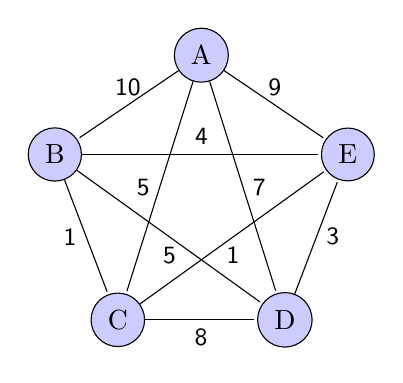
\begin{tikzpicture}[-,shorten >=1pt,auto,node distance=1.5cm,main node/.style={circle, draw, fill=blue!20}]
			
			\node[main node] (1) {A};
			\node[main node] (2) [below left of=1, xshift = -0.8cm, yshift = -0.2cm] {B};
			\node[main node] (3) [below of=2, xshift= 0.8cm, yshift = -0.6cm] {C};
			\node[main node] (5) [below right of=1, xshift = 0.8cm, yshift = -0.2cm] {E};
			\node[main node] (4) [below of=5, xshift= -0.8cm, yshift = -0.6cm] {D};
			
			
			
			\path[every node/.style={font=\sffamily\small}]
			(1)
			edge node [right] {7} (4)
			edge node[above] {10} (2)
			edge node[left] {5} (3)
			edge node[above] {9} (5)
			
			(2) 
			edge node[below] {5} (4)
			edge node[left] {1} (3)
			edge node[above] {4} (5)
			
			(3)
			edge node[below] {8} (4)
			edge node[below] {1} (5)
			
			(4) edge node[right] {3} (5);
			
		\end{tikzpicture}
		
	\end{center}
	
	
		\subsection{Algorithm Construction}
	
	We will follow the instructions highlighted at the begining of chapter 3. We start by normalizing our edge weights. We need to sort our all edge weights in descending order as in equation \ref{sorted-weights}:	
	
	\begin{equation*}
		w' = \{10,9,8,7,5,5,4,3,1,1\}
	\end{equation*}
	
	
	Then we need to retrieve the sum $S$ as in equation \ref{sum-S}
	\begin{equation*}
		S = \sum_{i=1}^{5} w'_i = 10 + 9  + 8 + 7 + 5 = 39
	\end{equation*}
	
	From here we can normalize our edgeweights as in \ref{normalization}, we can set $\epsilon = 1$
	
	\begin{equation*}
		\tilde{w} = \frac{  \{10,9,8,7,5,5,4,3,1,1\}}{40} = \{0.25 , 0.225 , 0.2 , 0.175 , 0.125, 0.125, 0.1, 0.075, 0.025, 0.025\} 
	\end{equation*}
	
	
	
	
	\begin{center}	
		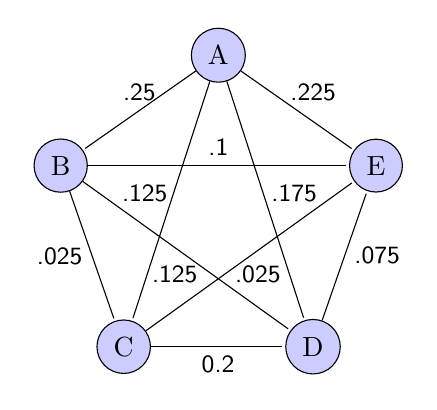
\begin{tikzpicture}[-,shorten >=1pt,auto,node distance=1.7cm,main node/.style={circle, draw, fill=blue!20}]
			
			\node[main node] (1) {A};
			\node[main node] (2) [below left of=1, xshift = -0.8cm, yshift = -0.2cm] {B};
			\node[main node] (3) [below of=2, xshift= 0.8cm, yshift = -0.6cm] {C};
			\node[main node] (5) [below right of=1, xshift = 0.8cm, yshift = -0.2cm] {E};
			\node[main node] (4) [below of=5, xshift= -0.8cm, yshift = -0.6cm] {D};
			
			
			
			\path[every node/.style={font=\sffamily\small}]
			(1)
			edge node [right, yshift = 0.1cm, xshift = -0.05cm] {.175} (4)
			edge node[above] {.25} (2)
			edge node[left, yshift = 0.1cm, xshift = 0.08cm] {.125} (3)
			edge node[above, xshift = 0.2cm] {.225} (5)
			
			(2) 
			edge node[below, xshift = -0.15cm] {.125} (4)
			edge node[left] {.025} (3)
			edge node[above] {.1} (5)
			
			(3)
			edge node[below] {0.2} (4)
			edge node[below, xshift = 0.1cm] {.025} (5)
			
			(4) edge node[right] {.075} (5);
			
		\end{tikzpicture}
		
	\end{center}
	
	
	
	Now we need to construct the unitary operator and eigenstates. Our matrix $U$ and $U'$ diagonals will look like the following:
	
	
	\begin{align*}	
		u & = \begin{bmatrix}
			1 \\
			e^{i2\pi(0.25)} \\
			e^{i2\pi(0.125)} \\
			e^{i2\pi(0.175)} \\
			e^{i2\pi(0.225)} \\
		\end{bmatrix} 
		\otimes \begin{bmatrix}
			e^{i2\pi(0.25)} \\
			1 \\
			e^{i2\pi(0.025)} \\
			e^{i2\pi(0.125)} \\
			e^{i2\pi(0.1)} \\
		\end{bmatrix}
		\otimes \begin{bmatrix}
			e^{i2\pi(0.125)} \\
			e^{i2\pi(0.025)} \\
			1\\
			e^{i2\pi(0.2)} \\
			e^{i2\pi(0.025)} \\
		\end{bmatrix} 
		\otimes \begin{bmatrix}
			e^{i2\pi(0.175)} \\
			e^{i2\pi(0.125)} \\
			e^{i2\pi(0.2)} \\
			1 \\
			e^{i2\pi(0.075)} \\
		\end{bmatrix} 
		\otimes \begin{bmatrix}
			e^{i2\pi(0.225)} \\
			e^{i2\pi(0.1)} \\
			e^{i2\pi(0.025)} \\
			e^{i2\pi(0.075)} \\
			1 \\
		\end{bmatrix} 							 			
	\end{align*}
	
	\begin{align*}	
	u' & = \begin{bmatrix}
		1 \\
		e^{i2\pi(0)} \\
		e^{i2\pi(0.125)} \\
		e^{i2\pi(0.175)} \\
		e^{i2\pi(0)} \\
	\end{bmatrix} 
	\otimes \begin{bmatrix}
		e^{i2\pi(0)} \\
		1 \\
		e^{i2\pi(0.025)} \\
		e^{i2\pi(0.125)} \\
		e^{i2\pi(0.1)} \\
	\end{bmatrix}
	\otimes \begin{bmatrix}
		e^{i2\pi(0.125)} \\
		e^{i2\pi(0.025)} \\
		1\\
		e^{i2\pi(0.2)} \\
		e^{i2\pi(0.025)} \\
	\end{bmatrix} 
	\otimes \begin{bmatrix}
		e^{i2\pi(0.175)} \\
		e^{i2\pi(0.125)} \\
		e^{i2\pi(0.2)} \\
		1 \\
		e^{i2\pi(0.075)} \\
	\end{bmatrix} 
	\otimes \begin{bmatrix}
		e^{i2\pi(0)} \\
		e^{i2\pi(0.1)} \\
		e^{i2\pi(0.025)} \\
		e^{i2\pi(0.075)} \\
		1 \\
	\end{bmatrix} 							 			
\end{align*}
	
	The number of diagonal elements in $U$ and $U'$ is $5^5 = 3125$ thus we need atleast $12$ eigenstate qubits to represent all $3125$ states. We will have left over states ($2^{12} - 5^5 = 971$). Thus to accomodate this issue we need to add $1$s to the end of the diagonal of matrices U and U'. With this method we do not affect the eigenstates. Then we can construct our block matrix structure shown in \ref{control-u-matrix} to create the controlled gates:
	
	\begin{equation}\label{ones}
	\mathrm{diag}(U) = [u, \mathrm{ones}(971)], \;\; \mathrm{diag}(U') = [u', \mathrm{ones}(971)]
	\end{equation}
\begin{equation*}
	CU = \begin{bmatrix}
		\mathbb{I}_{12} & 0 \\
		0 & U \\
	\end{bmatrix},\;\;\;
	CU' = \begin{bmatrix}
		\mathbb{I}_{12} & 0 \\
		0 & U' \\
	\end{bmatrix}
\end{equation*}	
	
	Because we are dealing with the symmetric case, we will only use half of the eigenstates listed in Table \ref{table:ham-cycle-details-5-city}:
	
	$$|970\rangle  = |001111001010\rangle$$
	$$|978\rangle  = |001111010010\rangle$$
	$$|1110\rangle = |010001010110\rangle$$
	$$|1022\rangle = |001111111110\rangle$$
	$$|1202\rangle = |010010110010\rangle$$
	$$|1138\rangle = |010001110010\rangle$$
	$$|1670\rangle = |011010000110\rangle$$
	$$|1778\rangle = |011011110010\rangle$$
	$$|1830\rangle = |011100100110\rangle$$
	$$|1726\rangle = |011010111110\rangle$$
	$$|2230\rangle = |100010110110\rangle$$
	$$|2410\rangle = |100101101010\rangle$$
	And expect the following phases:
	
		Cycle 1: $A \rightarrow B \rightarrow C \rightarrow D \rightarrow E \rightarrow A$.\;\;\;\;\;\;\;\;\;\;\;\;\;\; $u_{970}  = e^{i2\pi(0.775)}$, \;\;\;\;\;$u'_{970} = e^{i2\pi(0.3)}$
		
	\begin{center}	
		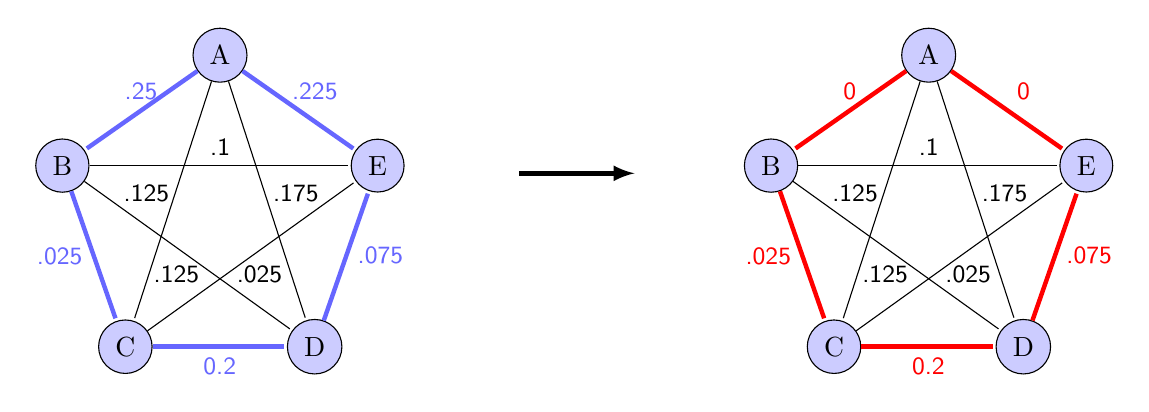
\begin{tikzpicture}[-,shorten >=1pt,auto,node distance=1.7cm,main node/.style={circle, draw, fill=blue!20}]
			% Nodes
			\node [main node] (1) at (0,0) {A};
			%\node[main node] (1) {A};
			\node[main node] (2) [below left of=1, xshift = -0.8cm, yshift = -0.2cm] {B};
			\node[main node] (3) [below of=2, xshift= 0.8cm, yshift = -0.6cm] {C};
			\node[main node] (5) [below right of=1, xshift = 0.8cm, yshift = -0.2cm] {E};
			\node[main node] (4) [below of=5, xshift= -0.8cm, yshift = -0.6cm] {D};
			
			
			
			\path[every node/.style={font=\sffamily\small}]
			(1)
			edge node [right, yshift = 0.1cm, xshift = -0.05cm] {.175} (4)
			edge[blue!60,ultra thick] node[above] {.25} (2)
			edge node[left, yshift = 0.1cm, xshift = 0.08cm] {.125} (3)
			edge[blue!60,ultra thick] node[above, xshift = 0.2cm] {.225} (5)
			
			(2) 
			edge node[below, xshift = -0.15cm] {.125} (4)
			edge[blue!60,ultra thick] node[left] {.025} (3)
			edge node[above] {.1} (5)
			
			(3)
			edge[blue!60,ultra thick] node[below] {0.2} (4)
			edge node[below, xshift = 0.1cm] {.025} (5)
			
			(4) edge [blue!60,ultra thick] node[right] {.075} (5);
			
			\node [main node] (6) at (9,0) {A};
			\node[main node] (7) [below left of=6, xshift = -0.8cm, yshift = -0.2cm] {B};
			\node[main node] (8) [below of=7, xshift= 0.8cm, yshift = -0.6cm] {C};
			\node[main node] (10) [below right of=6, xshift = 0.8cm, yshift = -0.2cm] {E};
			\node[main node] (9) [below of=10, xshift= -0.8cm, yshift = -0.6cm] {D};
			
			
			\path[every node/.style={font=\sffamily\small}]
			(6)
			edge node [right, yshift = 0.1cm, xshift = -0.05cm] {.175} (9)
			edge [red,ultra thick]node[above] {0} (7)
			edgenode[left, yshift = 0.1cm, xshift = 0.08cm] {.125} (8)
			edge[red,ultra thick] node[above, xshift = 0.2cm] {0} (10)
			
			(7) 
			edge node[below, xshift = -0.15cm] {.125} (9)
			edge[red,ultra thick] node[left] {.025} (8)
			edge node[above] {.1} (10)
			
			(8)
			edge [red,ultra thick] node[below] {0.2} (9)
			edge node[below, xshift = 0.1cm] {.025} (10)
			
			(9)edge[red,ultra thick]  node[right] {.075} (10);
			
			\draw[->, ultra thick, >=latex] (3.8, -1.5) -- (5.3, -1.5);
			
		\end{tikzpicture}
	\end{center}
	
	Cycle 2: $A \rightarrow B \rightarrow C \rightarrow E \rightarrow D \rightarrow A$.\;\;\;\;\;\;\;\;\;\;\;\;\;\; $ u_{978}  = e^{i2\pi(0.55)}$, \;\;\;\;\; $ u'_{978} = e^{i2\pi(0.3)}$
	\begin{center}	
		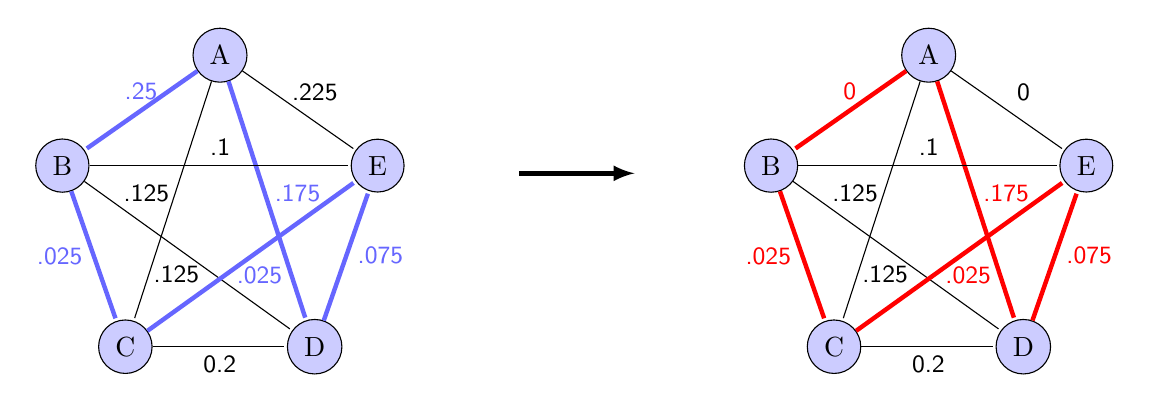
\begin{tikzpicture}[-,shorten >=1pt,auto,node distance=1.7cm,main node/.style={circle, draw, fill=blue!20}]
			% Nodes
			\node [main node] (1) at (0,0) {A};
			%\node[main node] (1) {A};
			\node[main node] (2) [below left of=1, xshift = -0.8cm, yshift = -0.2cm] {B};
			\node[main node] (3) [below of=2, xshift= 0.8cm, yshift = -0.6cm] {C};
			\node[main node] (5) [below right of=1, xshift = 0.8cm, yshift = -0.2cm] {E};
			\node[main node] (4) [below of=5, xshift= -0.8cm, yshift = -0.6cm] {D};
			
			
			
			\path[every node/.style={font=\sffamily\small}]
			(1)
			edge [blue!60,ultra thick]node [right, yshift = 0.1cm, xshift = -0.05cm] {.175} (4)
			edge [blue!60,ultra thick]node[above] {.25} (2)
			edge node[left, yshift = 0.1cm, xshift = 0.08cm] {.125} (3)
			edge node[above, xshift = 0.2cm] {.225} (5)
			
			(2) 
			edge node[below, xshift = -0.15cm] {.125} (4)
			edge [blue!60,ultra thick]node[left] {.025} (3)
			edge node[above] {.1} (5)
			
			(3)
			edge node[below] {0.2} (4)
			edge [blue!60,ultra thick]node[below, xshift = 0.1cm] {.025} (5)
			
			(4) edge[blue!60,ultra thick] node[right] {.075} (5);
			
			\node [main node] (6) at (9,0) {A};
			\node[main node] (7) [below left of=6, xshift = -0.8cm, yshift = -0.2cm] {B};
			\node[main node] (8) [below of=7, xshift= 0.8cm, yshift = -0.6cm] {C};
			\node[main node] (10) [below right of=6, xshift = 0.8cm, yshift = -0.2cm] {E};
			\node[main node] (9) [below of=10, xshift= -0.8cm, yshift = -0.6cm] {D};
			
			
			\path[every node/.style={font=\sffamily\small}]
			(6)
			edge [red,ultra thick] node [right, yshift = 0.1cm, xshift = -0.05cm] {.175} (9)
			edge[red,ultra thick] node[above] {0} (7)
			edge node[left, yshift = 0.1cm, xshift = 0.08cm] {.125} (8)
			edge node[above, xshift = 0.2cm] {0} (10)
			
			(7) 
			edge node[below, xshift = -0.15cm] {.125} (9)
			edge [red,ultra thick]node[left] {.025} (8)
			edge node[above] {.1} (10)
			
			(8)
			edge node[below] {0.2} (9)
			edge[red,ultra thick] node[below, xshift = 0.1cm] {.025} (10)
			
			(9)  edge [red,ultra thick] node[right] {.075} (10);
			
			\draw[->, ultra thick, >=latex] (3.8, -1.5) -- (5.3, -1.5);
			
		\end{tikzpicture}
	\end{center}

	
	Cycle 3: $A \rightarrow B \rightarrow D \rightarrow C \rightarrow E \rightarrow A$.\;\;\;\;\;\;\;\;\;\;\;\;\;\; $ u_{1110}  = e^{i2\pi(0.825)}$, \;\;\;\;\; $ u'_{1110} = e^{i2\pi(0.35)}$
	\begin{center}	
		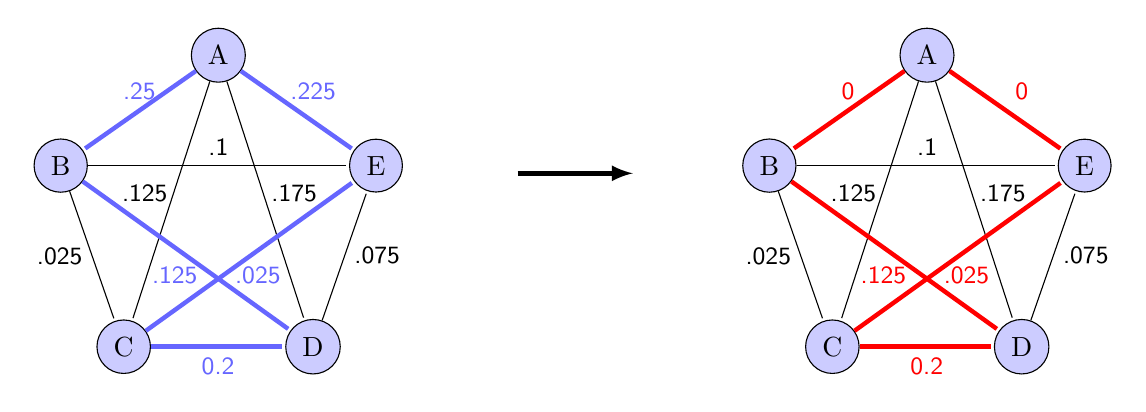
\begin{tikzpicture}[-,shorten >=1pt,auto,node distance=1.7cm,main node/.style={circle, draw, fill=blue!20}]
			% Nodes
			\node [main node] (1) at (0,0) {A};
			%\node[main node] (1) {A};
			\node[main node] (2) [below left of=1, xshift = -0.8cm, yshift = -0.2cm] {B};
			\node[main node] (3) [below of=2, xshift= 0.8cm, yshift = -0.6cm] {C};
			\node[main node] (5) [below right of=1, xshift = 0.8cm, yshift = -0.2cm] {E};
			\node[main node] (4) [below of=5, xshift= -0.8cm, yshift = -0.6cm] {D};
			
			
			
			\path[every node/.style={font=\sffamily\small}]
			(1)
			edge node [right, yshift = 0.1cm, xshift = -0.05cm] {.175} (4)
			edge [blue!60,ultra thick] node[above] {.25} (2)
			edge node[left, yshift = 0.1cm, xshift = 0.08cm] {.125} (3)
			edge[blue!60,ultra thick] node[above, xshift = 0.2cm] {.225} (5)
			
			(2) 
			edge[blue!60,ultra thick] node[below, xshift = -0.15cm] {.125} (4)
			edge node[left] {.025} (3)
			edge node[above] {.1} (5)
			
			(3)
			edge[blue!60,ultra thick] node[below] {0.2} (4)
			edge [blue!60,ultra thick]node[below, xshift = 0.1cm] {.025} (5)
			
			(4) edge node[right] {.075} (5);
			
			\node [main node] (6) at (9,0) {A};
			\node[main node] (7) [below left of=6, xshift = -0.8cm, yshift = -0.2cm] {B};
			\node[main node] (8) [below of=7, xshift= 0.8cm, yshift = -0.6cm] {C};
			\node[main node] (10) [below right of=6, xshift = 0.8cm, yshift = -0.2cm] {E};
			\node[main node] (9) [below of=10, xshift= -0.8cm, yshift = -0.6cm] {D};
			
			
			\path[every node/.style={font=\sffamily\small}]
			(6)
			edge node [right, yshift = 0.1cm, xshift = -0.05cm] {.175} (9)
			edge[red,ultra thick] node[above] {0} (7)
			edge node[left, yshift = 0.1cm, xshift = 0.08cm] {.125} (8)
			edge[red,ultra thick] node[above, xshift = 0.2cm] {0} (10)
			
			(7) 
			edge [red,ultra thick]node[below, xshift = -0.15cm] {.125} (9)
			edge node[left] {.025} (8)
			edge node[above] {.1} (10)
			
			(8)
			edge[red,ultra thick] node[below] {0.2} (9)
			edge[red,ultra thick] node[below, xshift = 0.1cm] {.025} (10)
			
			(9) edge node[right] {.075} (10);
			
			\draw[->, ultra thick, >=latex] (3.8, -1.5) -- (5.3, -1.5);
			
		\end{tikzpicture}
	\end{center}
	
		Cycle 4: $A \rightarrow B \rightarrow D \rightarrow E \rightarrow C \rightarrow A$.\;\;\;\;\;\;\;\;\;\;\;\;\;\; $ u_{1022}  = e^{i2\pi(0.6)}$, \;\;\;\;\; $ u'_{1022} = e^{i2\pi(0.35)}$
	\begin{center}	
		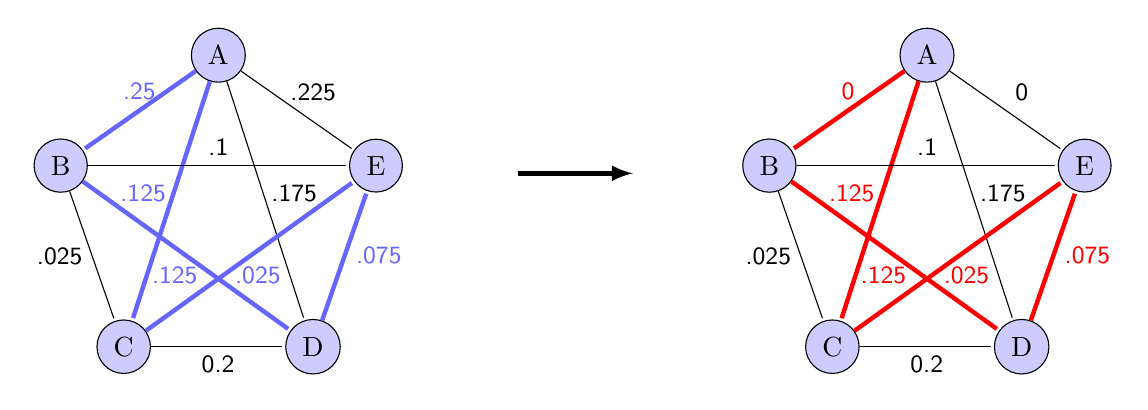
\begin{tikzpicture}[-,shorten >=1pt,auto,node distance=1.7cm,main node/.style={circle, draw, fill=blue!20}]
			% Nodes
			\node [main node] (1) at (0,0) {A};
			%\node[main node] (1) {A};
			\node[main node] (2) [below left of=1, xshift = -0.8cm, yshift = -0.2cm] {B};
			\node[main node] (3) [below of=2, xshift= 0.8cm, yshift = -0.6cm] {C};
			\node[main node] (5) [below right of=1, xshift = 0.8cm, yshift = -0.2cm] {E};
			\node[main node] (4) [below of=5, xshift= -0.8cm, yshift = -0.6cm] {D};
			
			
			
			\path[every node/.style={font=\sffamily\small}]
			(1)
			edge node [right, yshift = 0.1cm, xshift = -0.05cm] {.175} (4)
			edge[blue!60,ultra thick] node[above] {.25} (2)
			edge [blue!60,ultra thick] node[left, yshift = 0.1cm, xshift = 0.08cm] {.125} (3)
			edge node[above, xshift = 0.2cm] {.225} (5)
			
			(2) 
			edge [blue!60,ultra thick]node[below, xshift = -0.15cm] {.125} (4)
			edge node[left] {.025} (3)
			edge node[above] {.1} (5)
			
			(3)
			edge node[below] {0.2} (4)
			edge [blue!60,ultra thick]node[below, xshift = 0.1cm] {.025} (5)
			
			(4) edge [blue!60,ultra thick]node[right] {.075} (5);
			
			\node [main node] (6) at (9,0) {A};
			\node[main node] (7) [below left of=6, xshift = -0.8cm, yshift = -0.2cm] {B};
			\node[main node] (8) [below of=7, xshift= 0.8cm, yshift = -0.6cm] {C};
			\node[main node] (10) [below right of=6, xshift = 0.8cm, yshift = -0.2cm] {E};
			\node[main node] (9) [below of=10, xshift= -0.8cm, yshift = -0.6cm] {D};
			
			
			\path[every node/.style={font=\sffamily\small}]
			(6)
			edge node [right, yshift = 0.1cm, xshift = -0.05cm] {.175} (9)
			edge [red,ultra thick]node[above] {0} (7)
			edge [red,ultra thick]node[left, yshift = 0.1cm, xshift = 0.08cm] {.125} (8)
			edge node[above, xshift = 0.2cm] {0} (10)
			
			(7) 
			edge [red,ultra thick]node[below, xshift = -0.15cm] {.125} (9)
			edge node[left] {.025} (8)
			edge node[above] {.1} (10)
			
			(8)
			edge node[below] {0.2} (9)
			edge[red,ultra thick] node[below, xshift = 0.1cm] {.025} (10)
			
			(9) edge [red,ultra thick]node[right] {.075} (10);
			
			\draw[->, ultra thick, >=latex] (3.8, -1.5) -- (5.3, -1.5);
			
		\end{tikzpicture}
	\end{center}
	
		Cycle 5: $A \rightarrow B \rightarrow E \rightarrow C \rightarrow D \rightarrow A$.\;\;\;\;\;\;\;\;\;\;\;\;\;\; $ u_{1202}  = e^{i2\pi(0.75)}$, \;\;\;\;\; $ u'_{1202} = e^{i2\pi(0.5)}$
	\begin{center}	
		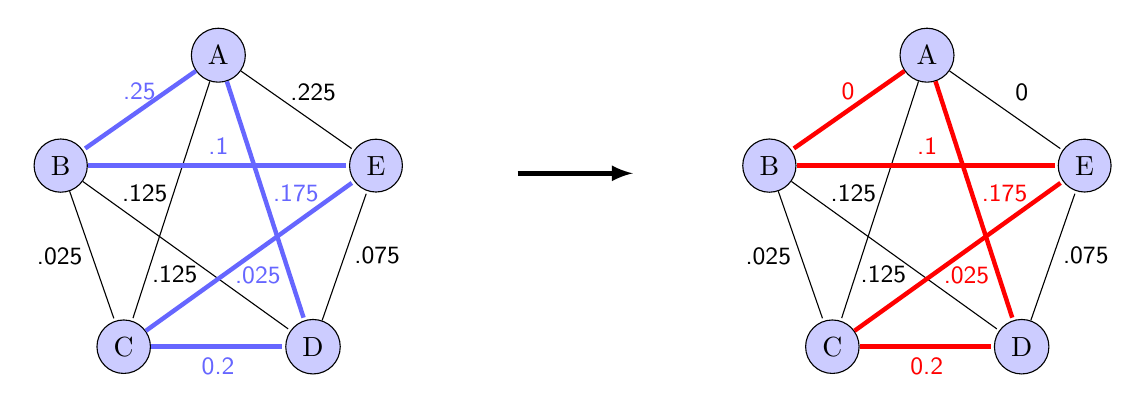
\begin{tikzpicture}[-,shorten >=1pt,auto,node distance=1.7cm,main node/.style={circle, draw, fill=blue!20}]
			% Nodes
			\node [main node] (1) at (0,0) {A};
			\node[main node] (2) [below left of=1, xshift = -0.8cm, yshift = -0.2cm] {B};
			\node[main node] (3) [below of=2, xshift= 0.8cm, yshift = -0.6cm] {C};
			\node[main node] (5) [below right of=1, xshift = 0.8cm, yshift = -0.2cm] {E};
			\node[main node] (4) [below of=5, xshift= -0.8cm, yshift = -0.6cm] {D};
			
			
			
			\path[every node/.style={font=\sffamily\small}]
			(1)
			edge  [blue!60,ultra thick]node [right, yshift = 0.1cm, xshift = -0.05cm] {.175} (4)
			edge [blue!60,ultra thick] node[above] {.25} (2)
			edge node[left, yshift = 0.1cm, xshift = 0.08cm] {.125} (3)
			edge node[above, xshift = 0.2cm] {.225} (5)
			
			(2) 
			edge node[below, xshift = -0.15cm] {.125} (4)
			edge node[left] {.025} (3)
			edge  [blue!60,ultra thick]node[above] {.1} (5)
			
			(3)
			edge  [blue!60,ultra thick]node[below] {0.2} (4)
			edge  [blue!60,ultra thick]node[below, xshift = 0.1cm] {.025} (5)
			
			(4) edge node[right] {.075} (5);
			
			\node [main node] (6) at (9,0) {A};
			\node[main node] (7) [below left of=6, xshift = -0.8cm, yshift = -0.2cm] {B};
			\node[main node] (8) [below of=7, xshift= 0.8cm, yshift = -0.6cm] {C};
			\node[main node] (10) [below right of=6, xshift = 0.8cm, yshift = -0.2cm] {E};
			\node[main node] (9) [below of=10, xshift= -0.8cm, yshift = -0.6cm] {D};
			
			
			\path[every node/.style={font=\sffamily\small}]
			(6)
			edge[red,ultra thick] node [right, yshift = 0.1cm, xshift = -0.05cm] {.175} (9)
			edge[red,ultra thick] node[above] {0} (7)
			edge node[left, yshift = 0.1cm, xshift = 0.08cm] {.125} (8)
			edge node[above, xshift = 0.2cm] {0} (10)
			
			(7) 
			edge node[below, xshift = -0.15cm] {.125} (9)
			edge node[left] {.025} (8)
			edge[red,ultra thick] node[above] {.1} (10)
			
			(8)
			edge [red,ultra thick]node[below] {0.2} (9)
			edge [red,ultra thick]node[below, xshift = 0.1cm] {.025} (10)
			
			(9) edge node[right] {.075} (10);
			
			\draw[->, ultra thick, >=latex] (3.8, -1.5) -- (5.3, -1.5);
			
		\end{tikzpicture}
	\end{center}
	
		Cycle 6: $A \rightarrow B \rightarrow E \rightarrow D \rightarrow C \rightarrow A$.\;\;\;\;\;\;\;\;\;\;\;\;\;\; $ u_{1138}  = e^{i2\pi(0.75)}$, \;\;\;\;\; $ u'_{1138} = e^{i2\pi(0.5)}$
	\begin{center}	
		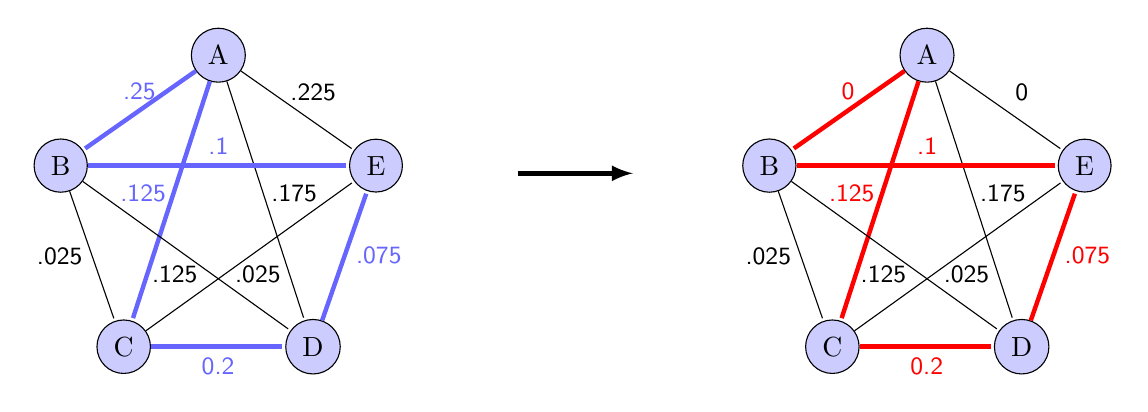
\begin{tikzpicture}[-,shorten >=1pt,auto,node distance=1.7cm,main node/.style={circle, draw, fill=blue!20}]
			% Nodes
			\node [main node] (1) at (0,0) {A};
			%\node[main node] (1) {A};
			\node[main node] (2) [below left of=1, xshift = -0.8cm, yshift = -0.2cm] {B};
			\node[main node] (3) [below of=2, xshift= 0.8cm, yshift = -0.6cm] {C};
			\node[main node] (5) [below right of=1, xshift = 0.8cm, yshift = -0.2cm] {E};
			\node[main node] (4) [below of=5, xshift= -0.8cm, yshift = -0.6cm] {D};
			
			
			
			\path[every node/.style={font=\sffamily\small}]
			(1)
			edge node [right, yshift = 0.1cm, xshift = -0.05cm] {.175} (4)
			edge [blue!60,ultra thick] node[above] {.25} (2)
			edge[blue!60,ultra thick]  node[left, yshift = 0.1cm, xshift = 0.08cm] {.125} (3)
			edge node[above, xshift = 0.2cm] {.225} (5)
			
			(2) 
			edge node[below, xshift = -0.15cm] {.125} (4)
			edge node[left] {.025} (3)
			edge  [blue!60,ultra thick] node[above] {.1} (5)
			
			(3)
			edge [blue!60,ultra thick]  node[below] {0.2} (4)
			edge node[below, xshift = 0.1cm] {.025} (5)
			
			(4)  edge[blue!60,ultra thick]  node[right] {.075} (5);
			
			\node [main node] (6) at (9,0) {A};
			\node[main node] (7) [below left of=6, xshift = -0.8cm, yshift = -0.2cm] {B};
			\node[main node] (8) [below of=7, xshift= 0.8cm, yshift = -0.6cm] {C};
			\node[main node] (10) [below right of=6, xshift = 0.8cm, yshift = -0.2cm] {E};
			\node[main node] (9) [below of=10, xshift= -0.8cm, yshift = -0.6cm] {D};
			
			
			\path[every node/.style={font=\sffamily\small}]
			(6)
			edge node [right, yshift = 0.1cm, xshift = -0.05cm] {.175} (9)
			edge[red,ultra thick] node[above] {0} (7)
			edge [red,ultra thick]node[left, yshift = 0.1cm, xshift = 0.08cm] {.125} (8)
			edge node[above, xshift = 0.2cm] {0} (10)
			
			(7) 
			edge node[below, xshift = -0.15cm] {.125} (9)
			edge node[left] {.025} (8)
			edge [red,ultra thick]node[above] {.1} (10)
			
			(8)
			edge[red,ultra thick] node[below] {0.2} (9)
			edge node[below, xshift = 0.1cm] {.025} (10)
			
			(9) edge[red,ultra thick] node[right] {.075} (10);
			
			\draw[->, ultra thick, >=latex] (3.8, -1.5) -- (5.3, -1.5);
			
		\end{tikzpicture}
	\end{center}
	
		Cycle 7: $A \rightarrow C \rightarrow B \rightarrow D \rightarrow E \rightarrow A$.\;\;\;\;\;\;\;\;\;\;\;\;\;\; $ u_{1670}  = e^{i2\pi(0.575)}$, \;\;\;\;\; $ u'_{1670} = e^{i2\pi(0.35)}$
	\begin{center}	
		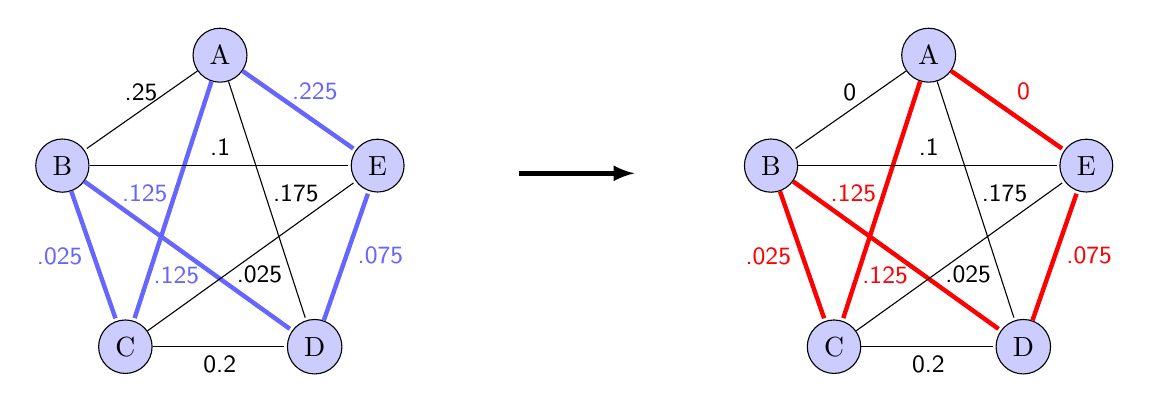
\begin{tikzpicture}[-,shorten >=1pt,auto,node distance=1.7cm,main node/.style={circle, draw, fill=blue!20}]
			% Nodes
			\node [main node] (1) at (0,0) {A};
			%\node[main node] (1) {A};
			\node[main node] (2) [below left of=1, xshift = -0.8cm, yshift = -0.2cm] {B};
			\node[main node] (3) [below of=2, xshift= 0.8cm, yshift = -0.6cm] {C};
			\node[main node] (5) [below right of=1, xshift = 0.8cm, yshift = -0.2cm] {E};
			\node[main node] (4) [below of=5, xshift= -0.8cm, yshift = -0.6cm] {D};
			
			
			
			\path[every node/.style={font=\sffamily\small}]
			(1)
			edge node [right, yshift = 0.1cm, xshift = -0.05cm] {.175} (4)
			edge node[above] {.25} (2)
			edge [blue!60,ultra thick] node[left, yshift = 0.1cm, xshift = 0.08cm] {.125} (3)
			edge [blue!60,ultra thick] node[above, xshift = 0.2cm] {.225} (5)
			
			(2) 
			edge [blue!60,ultra thick] node[below, xshift = -0.15cm] {.125} (4)
			edge [blue!60,ultra thick]  node[left] {.025} (3)
			edge node[above] {.1} (5)
			
			(3)
			edge node[below] {0.2} (4)
			edge node[below, xshift = 0.1cm] {.025} (5)
			
			(4) edge [blue!60,ultra thick]  node[right] {.075} (5);
			
			\node [main node] (6) at (9,0) {A};
			\node[main node] (7) [below left of=6, xshift = -0.8cm, yshift = -0.2cm] {B};
			\node[main node] (8) [below of=7, xshift= 0.8cm, yshift = -0.6cm] {C};
			\node[main node] (10) [below right of=6, xshift = 0.8cm, yshift = -0.2cm] {E};
			\node[main node] (9) [below of=10, xshift= -0.8cm, yshift = -0.6cm] {D};
			
			
			\path[every node/.style={font=\sffamily\small}]
			(6)
			edge node [right, yshift = 0.1cm, xshift = -0.05cm] {.175} (9)
			edge node[above] {0} (7)
			edge [red,ultra thick]node[left, yshift = 0.1cm, xshift = 0.08cm] {.125} (8)
			edge [red,ultra thick]node[above, xshift = 0.2cm] {0} (10)
			
			(7) 
			edge [red,ultra thick]node[below, xshift = -0.15cm] {.125} (9)
			edge [red,ultra thick]node[left] {.025} (8)
			edge node[above] {.1} (10)
			
			(8)
			edge node[below] {0.2} (9)
			edge node[below, xshift = 0.1cm] {.025} (10)
			
			(9) edge[red,ultra thick] node[right] {.075} (10);
			
			\draw[->, ultra thick, >=latex] (3.8, -1.5) -- (5.3, -1.5);
			
		\end{tikzpicture}
	\end{center}
	
		 Cycle 8: $A \rightarrow C \rightarrow B \rightarrow E \rightarrow D \rightarrow A$.\;\;\;\;\;\;\;\;\;\;\;\;\;\; $ u_{1778}  = e^{i2\pi(0.5)}$, \;\;\;\;\; $ u'_{1778}  = e^{i2\pi(0.5)}$
	
	\begin{center}	
		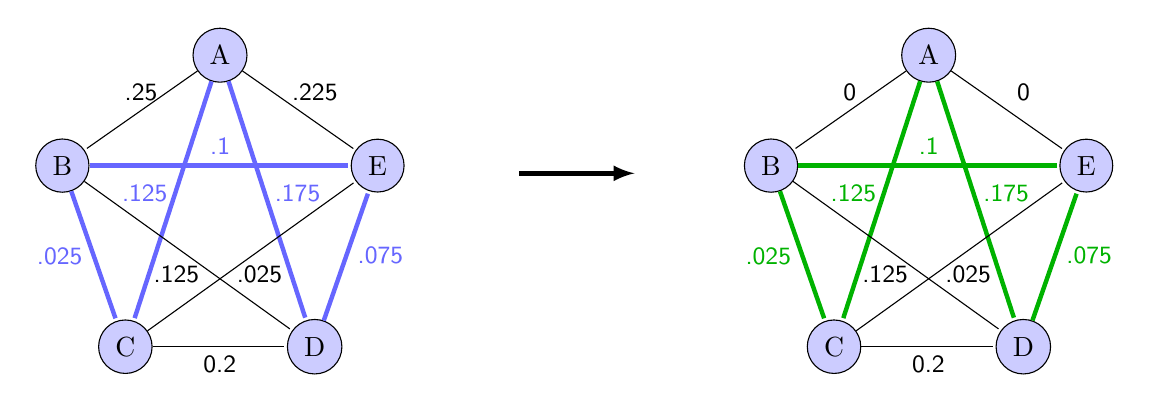
\begin{tikzpicture}[-,shorten >=1pt,auto,node distance=1.7cm,main node/.style={circle, draw, fill=blue!20}]
			% Nodes
			\node [main node] (1) at (0,0) {A};
			%\node[main node] (1) {A};
			\node[main node] (2) [below left of=1, xshift = -0.8cm, yshift = -0.2cm] {B};
			\node[main node] (3) [below of=2, xshift= 0.8cm, yshift = -0.6cm] {C};
			\node[main node] (5) [below right of=1, xshift = 0.8cm, yshift = -0.2cm] {E};
			\node[main node] (4) [below of=5, xshift= -0.8cm, yshift = -0.6cm] {D};
			
			
			
			\path[every node/.style={font=\sffamily\small}]
			(1)
			edge[blue!60,ultra thick] node [right, yshift = 0.1cm, xshift = -0.05cm] {.175} (4)
			edge node[above] {.25} (2)
			edge[blue!60,ultra thick] node[left, yshift = 0.1cm, xshift = 0.08cm] {.125} (3)
			edge node[above, xshift = 0.2cm] {.225} (5)
			
			(2) 
			edge node[below, xshift = -0.15cm] {.125} (4)
			edge[blue!60,ultra thick] node[left] {.025} (3)
			edge[blue!60,ultra thick] node[above] {.1} (5)
			
			(3)
			edge node[below] {0.2} (4)
			edge node[below, xshift = 0.1cm] {.025} (5)
			
			(4) edge[blue!60,ultra thick]  node[right] {.075} (5);
			
			
			
			\node [main node] (6) at (9,0) {A};
			\node[main node] (7) [below left of=6, xshift = -0.8cm, yshift = -0.2cm] {B};
			\node[main node] (8) [below of=7, xshift= 0.8cm, yshift = -0.6cm] {C};
			\node[main node] (10) [below right of=6, xshift = 0.8cm, yshift = -0.2cm] {E};
			\node[main node] (9) [below of=10, xshift= -0.8cm, yshift = -0.6cm] {D};
			
			
			
			\path[every node/.style={font=\sffamily\small}]
			(6)
			edge[black!30!green, ultra thick] node [right, yshift = 0.1cm, xshift = -0.05cm] {.175} (9)
			edge node[above] {0} (7)
			edge[black!30!green, ultra thick] node[left, yshift = 0.1cm, xshift = 0.08cm] {.125} (8)
			edge node[above, xshift = 0.2cm] {0} (10)
			
			(7) 
			edge node[below, xshift = -0.15cm] {.125} (9)
			edge[black!30!green, ultra thick] node[left] {.025} (8)
			edge[black!30!green, ultra thick] node[above] {.1} (10)
			
			(8)
			edge node[below] {0.2} (9)
			edge node[below, xshift = 0.1cm] {.025} (10)
			
			(9) edge[black!30!green, ultra thick] node[right] {.075} (10);
			
			\draw[->, ultra thick, >=latex] (3.8, -1.5) -- (5.3, -1.5);
			
		\end{tikzpicture}
	\end{center}
	
	
	Cycle 9: $A \rightarrow C \rightarrow D \rightarrow B \rightarrow E \rightarrow A$.\;\;\;\;\;\;\;\;\;\;\;\;\;\; $ u_{1830} =  e^{i2\pi(0.775)}$, \;\;\;\;\; $ u'_{1830} =  e^{i2\pi(0.55)}$
	
		\begin{center}	
		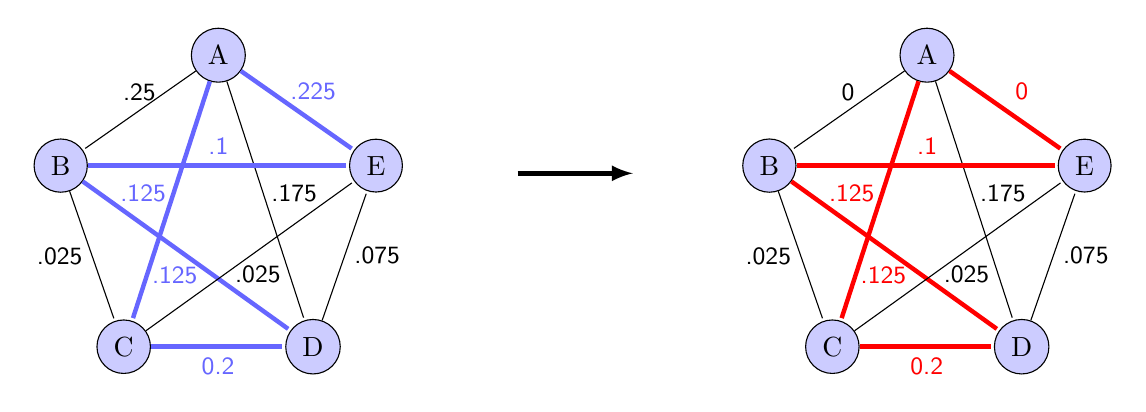
\begin{tikzpicture}[-,shorten >=1pt,auto,node distance=1.7cm,main node/.style={circle, draw, fill=blue!20}]
			% Nodes
			\node [main node] (1) at (0,0) {A};
			%\node[main node] (1) {A};
			\node[main node] (2) [below left of=1, xshift = -0.8cm, yshift = -0.2cm] {B};
			\node[main node] (3) [below of=2, xshift= 0.8cm, yshift = -0.6cm] {C};
			\node[main node] (5) [below right of=1, xshift = 0.8cm, yshift = -0.2cm] {E};
			\node[main node] (4) [below of=5, xshift= -0.8cm, yshift = -0.6cm] {D};
			
			
			
			\path[every node/.style={font=\sffamily\small}]
			(1)
			edge node [right, yshift = 0.1cm, xshift = -0.05cm] {.175} (4)
			edge node[above] {.25} (2)
			edge[blue!60,ultra thick] node[left, yshift = 0.1cm, xshift = 0.08cm] {.125} (3)
			edge[blue!60,ultra thick] node[above, xshift = 0.2cm] {.225} (5)
			
			(2) 
			edge[blue!60,ultra thick] node[below, xshift = -0.15cm] {.125} (4)
			edge node[left] {.025} (3)
			edge[blue!60,ultra thick] node[above] {.1} (5)
			
			(3)
			edge[blue!60,ultra thick] node[below] {0.2} (4)
			edge node[below, xshift = 0.1cm] {.025} (5)
			
			(4) edge node[right] {.075} (5);
			
			\node [main node] (6) at (9,0) {A};
			\node[main node] (7) [below left of=6, xshift = -0.8cm, yshift = -0.2cm] {B};
			\node[main node] (8) [below of=7, xshift= 0.8cm, yshift = -0.6cm] {C};
			\node[main node] (10) [below right of=6, xshift = 0.8cm, yshift = -0.2cm] {E};
			\node[main node] (9) [below of=10, xshift= -0.8cm, yshift = -0.6cm] {D};
			

			\path[every node/.style={font=\sffamily\small}]
			(6)
			edge node [right, yshift = 0.1cm, xshift = -0.05cm] {.175} (9)
			edge node[above] {0} (7)
			edge[red,ultra thick] node[left, yshift = 0.1cm, xshift = 0.08cm] {.125} (8)
			edge [red,ultra thick]node[above, xshift = 0.2cm] {0} (10)
			
			(7) 
			edge [red,ultra thick]node[below, xshift = -0.15cm] {.125} (9)
			edge node[left] {.025} (8)
			edge[red,ultra thick] node[above] {.1} (10)
			
			(8)
			edge [red,ultra thick]node[below] {0.2} (9)
			edge node[below, xshift = 0.1cm] {.025} (10)
			
			(9) edge node[right] {.075} (10);
			
			\draw[->, ultra thick, >=latex] (3.8, -1.5) -- (5.3, -1.5);
			
		\end{tikzpicture}
	\end{center}
	
		Cycle 10: $A \rightarrow C \rightarrow E \rightarrow B \rightarrow D \rightarrow A$.\;\;\;\;\;\;\;\;\;\;\;\;\;\; $ u_{1726} =  e^{i2\pi(0.55)}$, \;\;\;\;\; $ u'_{1726} = e^{i2\pi(0.55)}$
	
	\begin{center}	
		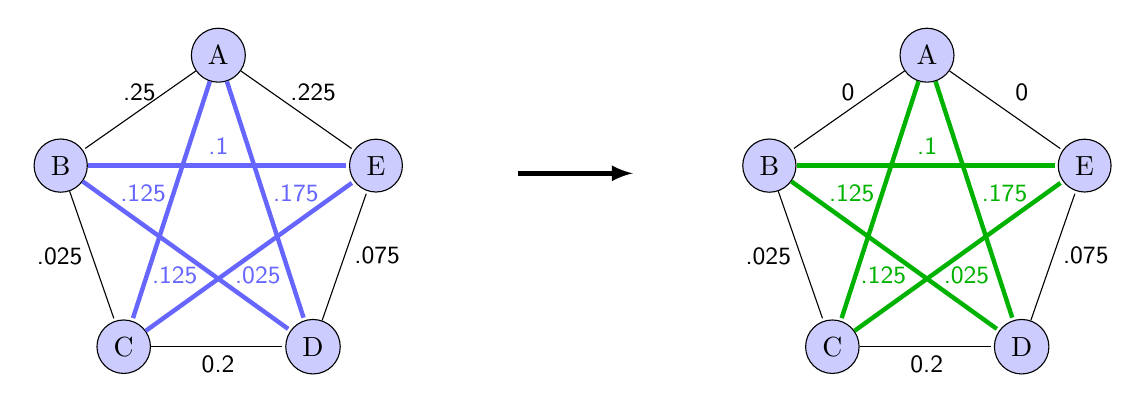
\begin{tikzpicture}[-,shorten >=1pt,auto,node distance=1.7cm,main node/.style={circle, draw, fill=blue!20}]
			% Nodes
			\node [main node] (1) at (0,0) {A};
			%\node[main node] (1) {A};
			\node[main node] (2) [below left of=1, xshift = -0.8cm, yshift = -0.2cm] {B};
			\node[main node] (3) [below of=2, xshift= 0.8cm, yshift = -0.6cm] {C};
			\node[main node] (5) [below right of=1, xshift = 0.8cm, yshift = -0.2cm] {E};
			\node[main node] (4) [below of=5, xshift= -0.8cm, yshift = -0.6cm] {D};
			
			
			
			\path[every node/.style={font=\sffamily\small}]
			(1)
			edge[blue!60,ultra thick] node [right, yshift = 0.1cm, xshift = -0.05cm] {.175} (4)
			edge node[above] {.25} (2)
			edge[blue!60,ultra thick] node[left, yshift = 0.1cm, xshift = 0.08cm] {.125} (3)
			edge node[above, xshift = 0.2cm] {.225} (5)
			
			(2) 
			edge[blue!60,ultra thick] node[below, xshift = -0.15cm] {.125} (4)
			edge node[left] {.025} (3)
			edge[blue!60,ultra thick] node[above] {.1} (5)
			
			(3)
			edge node[below] {0.2} (4)
			edge[blue!60,ultra thick] node[below, xshift = 0.1cm] {.025} (5)
			
			(4) edge node[right] {.075} (5);
			
			\node [main node] (6) at (9,0) {A};
			\node[main node] (7) [below left of=6, xshift = -0.8cm, yshift = -0.2cm] {B};
			\node[main node] (8) [below of=7, xshift= 0.8cm, yshift = -0.6cm] {C};
			\node[main node] (10) [below right of=6, xshift = 0.8cm, yshift = -0.2cm] {E};
			\node[main node] (9) [below of=10, xshift= -0.8cm, yshift = -0.6cm] {D};
			
			
			\path[every node/.style={font=\sffamily\small}]
			(6)
			edge [black!30!green, ultra thick]node [right, yshift = 0.1cm, xshift = -0.05cm] {.175} (9)
			edge node[above] {0} (7)
			edge[black!30!green, ultra thick] node[left, yshift = 0.1cm, xshift = 0.08cm] {.125} (8)
			edge node[above, xshift = 0.2cm] {0} (10)
			
			(7) 
			edge[black!30!green, ultra thick] node[below, xshift = -0.15cm] {.125} (9)
			edge node[left] {.025} (8)
			edge[black!30!green, ultra thick] node[above] {.1} (10)
			
			(8)
			edge node[below] {0.2} (9)
			edge[black!30!green, ultra thick] node[below, xshift = 0.1cm] {.025} (10)
			
			(9) edge node[right] {.075} (10);
			
			\draw[->, ultra thick, >=latex] (3.8, -1.5) -- (5.3, -1.5);
			
		\end{tikzpicture}
	\end{center}

	
		Cycle 11: $A \rightarrow D \rightarrow B \rightarrow C \rightarrow E \rightarrow A$.\;\;\;\;\;\;\;\;\;\;\;\;\;\; $ u_{2230} =  e^{i2\pi(0.575)}$, \;\;\;\;\; $ u'_{2230} = e^{i2\pi(0.35)}$
	
	\begin{center}	
		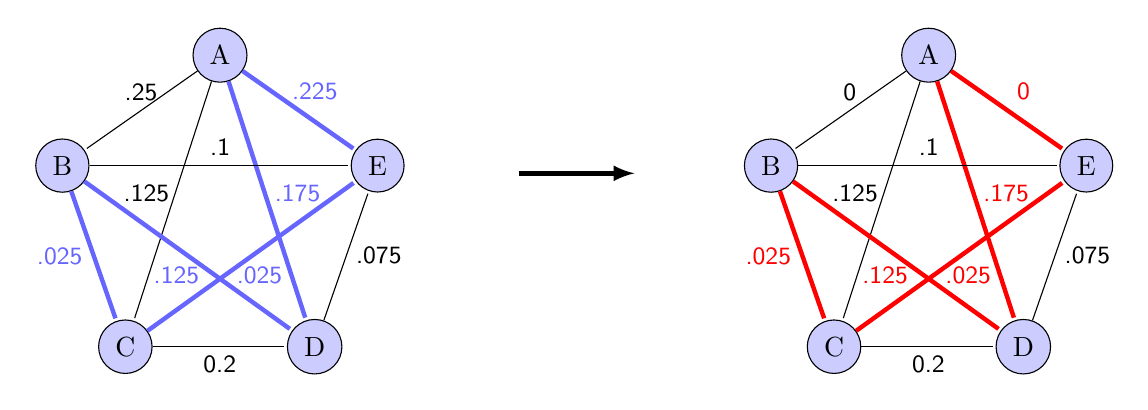
\begin{tikzpicture}[-,shorten >=1pt,auto,node distance=1.7cm,main node/.style={circle, draw, fill=blue!20}]
			% Nodes
			\node [main node] (1) at (0,0) {A};
			%\node[main node] (1) {A};
			\node[main node] (2) [below left of=1, xshift = -0.8cm, yshift = -0.2cm] {B};
			\node[main node] (3) [below of=2, xshift= 0.8cm, yshift = -0.6cm] {C};
			\node[main node] (5) [below right of=1, xshift = 0.8cm, yshift = -0.2cm] {E};
			\node[main node] (4) [below of=5, xshift= -0.8cm, yshift = -0.6cm] {D};
			
			
			
			\path[every node/.style={font=\sffamily\small}]
			(1)
			edge[blue!60,ultra thick] node [right, yshift = 0.1cm, xshift = -0.05cm] {.175} (4)
			edge node[above] {.25} (2)
			edge node[left, yshift = 0.1cm, xshift = 0.08cm] {.125} (3)
			edge[blue!60,ultra thick] node[above, xshift = 0.2cm] {.225} (5)
			
			(2) 
			edge[blue!60,ultra thick] node[below, xshift = -0.15cm] {.125} (4)
			edge[blue!60,ultra thick] node[left] {.025} (3)
			edge node[above] {.1} (5)
			
			(3)
			edge node[below] {0.2} (4)
			edge[blue!60,ultra thick] node[below, xshift = 0.1cm] {.025} (5)
			
			(4) edge node[right] {.075} (5);
			
			\node [main node] (6) at (9,0) {A};
			\node[main node] (7) [below left of=6, xshift = -0.8cm, yshift = -0.2cm] {B};
			\node[main node] (8) [below of=7, xshift= 0.8cm, yshift = -0.6cm] {C};
			\node[main node] (10) [below right of=6, xshift = 0.8cm, yshift = -0.2cm] {E};
			\node[main node] (9) [below of=10, xshift= -0.8cm, yshift = -0.6cm] {D};
			
			
			\path[every node/.style={font=\sffamily\small}]
			(6)
			edge[red,ultra thick] node [right, yshift = 0.1cm, xshift = -0.05cm] {.175} (9)
			edge node[above] {0} (7)
			edge node[left, yshift = 0.1cm, xshift = 0.08cm] {.125} (8)
			edge [red,ultra thick]node[above, xshift = 0.2cm] {0} (10)
			
			(7) 
			edge[red,ultra thick] node[below, xshift = -0.15cm] {.125} (9)
			edge [red,ultra thick]node[left] {.025} (8)
			edge node[above] {.1} (10)
			
			(8)
			edge node[below] {0.2} (9)
			edge [red,ultra thick]node[below, xshift = 0.1cm] {.025} (10)
			
			(9) edge node[right] {.075} (10);
			
			\draw[->, ultra thick, >=latex] (3.8, -1.5) -- (5.3, -1.5);
			
		\end{tikzpicture}
	\end{center}
	
		Cycle 12: $A \rightarrow D \rightarrow C \rightarrow B \rightarrow E \rightarrow A$.\;\;\;\;\;\;\;\;\;\;\;\;\;\; $ u_{2410}  = e^{i2\pi(0.725)}$, \;\;\;\;\; $ u'_{2410}  = e^{i2\pi(0.5)}$
	
	\begin{center}	
		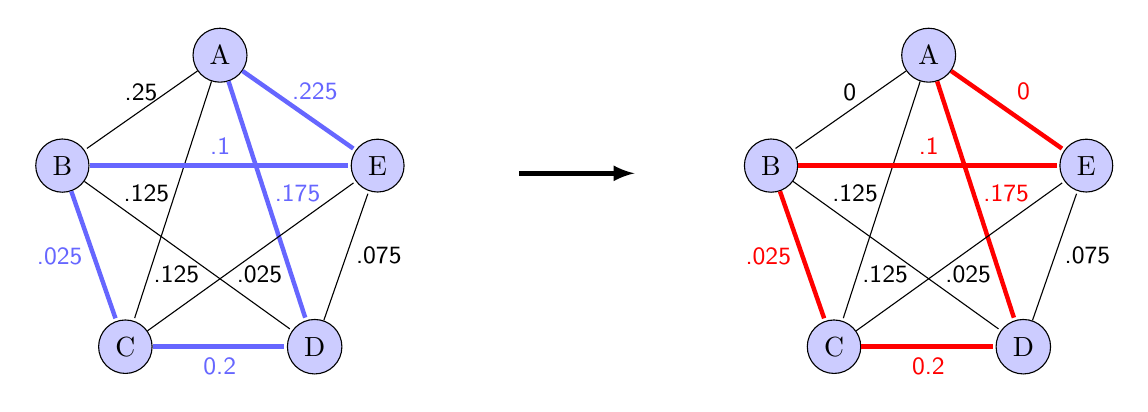
\begin{tikzpicture}[-,shorten >=1pt,auto,node distance=1.7cm,main node/.style={circle, draw, fill=blue!20}]
			% Nodes
			\node [main node] (1) at (0,0) {A};
			%\node[main node] (1) {A};
			\node[main node] (2) [below left of=1, xshift = -0.8cm, yshift = -0.2cm] {B};
			\node[main node] (3) [below of=2, xshift= 0.8cm, yshift = -0.6cm] {C};
			\node[main node] (5) [below right of=1, xshift = 0.8cm, yshift = -0.2cm] {E};
			\node[main node] (4) [below of=5, xshift= -0.8cm, yshift = -0.6cm] {D};
			
			
			
			\path[every node/.style={font=\sffamily\small}]
			(1)
			edge [blue!60,ultra thick]node [right, yshift = 0.1cm, xshift = -0.05cm] {.175} (4)
			edge node[above] {.25} (2)
			edge node[left, yshift = 0.1cm, xshift = 0.08cm] {.125} (3)
			edge [blue!60,ultra thick]node[above, xshift = 0.2cm] {.225} (5)
			
			(2) 
			edge node[below, xshift = -0.15cm] {.125} (4)
			edge[blue!60,ultra thick] node[left] {.025} (3)
			edge [blue!60,ultra thick]node[above] {.1} (5)
			
			(3)
			edge [blue!60,ultra thick]node[below] {0.2} (4)
			edge node[below, xshift = 0.1cm] {.025} (5)
			
			(4) edge node[right] {.075} (5);
			
			\node [main node] (6) at (9,0) {A};
			\node[main node] (7) [below left of=6, xshift = -0.8cm, yshift = -0.2cm] {B};
			\node[main node] (8) [below of=7, xshift= 0.8cm, yshift = -0.6cm] {C};
			\node[main node] (10) [below right of=6, xshift = 0.8cm, yshift = -0.2cm] {E};
			\node[main node] (9) [below of=10, xshift= -0.8cm, yshift = -0.6cm] {D};
			
			
			\path[every node/.style={font=\sffamily\small}]
			(6)
			edge[red,ultra thick] node [right, yshift = 0.1cm, xshift = -0.05cm] {.175} (9)
			edge node[above] {0} (7)
			edge node[left, yshift = 0.1cm, xshift = 0.08cm] {.125} (8)
			edge[red,ultra thick] node[above, xshift = 0.2cm] {0} (10)
			
			(7) 
			edge node[below, xshift = -0.15cm] {.125} (9)
			edge [red,ultra thick]node[left] {.025} (8)
			edge [red,ultra thick]node[above] {.1} (10)
			
			(8)
			edge [red,ultra thick]node[below] {0.2} (9)
			edge node[below, xshift = 0.1cm] {.025} (10)
			
			(9) edge node[right] {.075} (10);
			
			\draw[->, ultra thick, >=latex] (3.8, -1.5) -- (5.3, -1.5);
			
		\end{tikzpicture}
	\end{center}
	
		\subsection{Results: Simulations with Qiskit}  \label{5-city-sim}
	
	Fig. \ref{fig:5-city-circuit} shows us the circuit for our first hamiltonian cycle initialized in eigenstate $|970\rangle  = |001111001010\rangle$. We will run a similiar circuit for the other two hamiltonian cycles with the only change being the eigenstate initialization. We conduct an ideal simulation implying our results are not impacted by noise. Each circuit by default is run $1024$ times which we can use as a quasi-probability distribution. 
	
	\begin{figure}[!h]
		\centering
		\includegraphics[trim={8.5cm 4.4cm 6cm 4.4cm},clip, width=1 \linewidth]{"graphics/5-city-1-cycle-constrained-barrier"}
		\caption{the quantum circuit for the BTSP: 3 qubit phase estimation is performed measuring the hamiltonian cycle $A \rightarrow B \rightarrow C \rightarrow D \rightarrow E \rightarrow A$, using the corresponding eigenstate is $|970\rangle  = |001111001010\rangle$. Due to Qiskit convention on qubit ordering, the eigentate is initialized in reverse. The CU gate denotes the control unitary matrix containing all the hamiltonian cycles. The CU' gate inhabits the same cycles but before it was constructed, all edgeweights not satisfying the constraint, $\geq \alpha$, were set to zero. We have two sets of 3 qubits to be measured and stored in to classical registers labelled 'output' and 'output c'.}
		\label{fig:5-city-circuit}
	\end{figure}
	
	As we did for the 4-city graph, we present the top two counts (states?) for each hamiltonian cycle. 4-qubit estimation was performed as well. This results can be found in table \ref{table:sim-results-5-city}.
	
		\begin{figure}[!h]
		\centering
		\includegraphics[width=\textwidth,height=0.9\textheight,keepaspectratio]{"graphics/1-3-5city"}
		\caption{3 qubit (left column) \& 4 qubit (right column) phase estimation for the 5-city graph. Hamiltonian cycles: 1 to 3}
		\label{fig:5-city-1-3}
	\end{figure}		
	
	\begin{figure}[!h]
		\centering
		\includegraphics[ width=\textwidth,height=0.9\textheight,keepaspectratio]{"graphics/4-6-5city"}
		\caption{3 qubit (left column) \& 4 qubit (right column) phase estimation for the 5-city graph. Hamiltonian cycles: 4 to 6}
		\label{fig:5-city-4-6}
	\end{figure}		
	
	\begin{figure}[!h]
		\centering
		\includegraphics[width=\textwidth,height=0.9\textheight,keepaspectratio]{"graphics/7-9-5city"}
		\caption{3 qubit (left column) \& 4 qubit (right column) phase estimation for the 5-city graph. Hamiltonian cycles: 7 to 9}
		\label{fig:5-city-7-9}
	\end{figure}		
	
	\begin{figure}[!h]
		\centering
		\includegraphics[width=\textwidth,height=0.9\textheight,keepaspectratio]{"graphics/10-12-5city"}
		\caption{3 qubit (left column) \& 4 qubit (right column) phase estimation for the 5-city graph. Hamiltonian cycles: 10 to 12}
		\label{fig:5-city-10-12}
	\end{figure}		
	
	\begin{table}[ht!]
		\centering
		\label{your-table-label}
		\begin{tabular}{lllllll} % Updated for 7 columns
			\toprule
					Cycle & Expected & Phase Qubits & Highest Counts & Prob. & 2nd Highest Counts & Prob. \\
			\midrule
			\multirow{2}{*}{1} & \multirow{2}{*}{$0.3, \; 0.775$} & 3 & $0.25, \; 0.75$ & $52\%$ &  $0.375, \; 0.75$  & $23\%$ \\
			&                          & 4& $0.3125, \; 0.75$ & $50\%$ &  $0.3125, \; 0.8125$  & $21\%$ \\
			\hline
			\multirow{2}{*}{2} & \multirow{2}{*}{$0.3, \; 0.55$} & 3 & $0.25, \; 0.5$ & $35\%$ &  $0.25, \; 0.625$  & $14\%$ \\
			&                          & 4& $0.3125, \; 0.5625$ & $75\%$ &  $0.3125, \; 0.5$  & $6\%$ \\
			\hline
			\multirow{2}{*}{3} & \multirow{2}{*}{$0.35, \; 0.825$ } & 3 & $0.375, \; 0.875$ & $50\%$ &  $0.375, \; 0.75$  & $24\%$ \\
			&                          & 4& $0.375, \; 0.8125$ & $47\%$ &  $0.3125, \; 0.8125$  & $23\%$ \\
			\hline
			\multirow{2}{*}{4} & \multirow{2}{*}{$0.35, \; 0.6$} & 3 & $0.375, \; 0.625$ & $78\%$ &  $0.25, \; 0.625$  & $5\%$ \\
			&                          & 4& $0.375, \; 0.625$ & $31\%$ &  $0.3125, \; 0.625$  & $16\%$ \\
			\hline
			\multirow{2}{*}{5} & \multirow{2}{*}{$0.5, \; 0.75$} & 3 & $0.5, \; 0.75$ & $100\%$ & & \\
			&                          & 4& $0.5, \; 0.75$ & $100\%$ &   &  \\
			\hline
			\multirow{2}{*}{6} & \multirow{2}{*}{$0.5, \; 0.75$} & 3 & $0.5, \; 0.75$ & $100\%$ & & \\
			&                          & 4& $0.5, \; 0.75$ & $100\%$ &   &  \\
			\hline
			\multirow{2}{*}{7} & \multirow{2}{*}{$0.35, \; 0.575$ } & 3 & $0.375, \; 0.625$ & $51\%$ &  $0.375, \; 0.5$  & $23\%$ \\
			&                          & 4& $0.375, \; 0.5625$ & $50\%$ &  $0.3125, \; 0.5625$  & $21\%$ \\
			\hline
			\multirow{2}{*}{8} & \multirow{2}{*}{$0.5, \; 0.5$} & 3 & $0.5, \; 0.5$ & $100\%$ &   &  \\
			&                          & 4& $0.5, \; 0.5$ & $100\%$ &   &  \\
			\hline
			\multirow{2}{*}{9} & \multirow{2}{*}{$0.55, \; 0.775$} & 3 & $0.5, \; 0.75$ & $52\%$ &  $0.625, \; 0.75$  & $22\%$ \\
			&                          & 4& $0.5625, \; 0.75$ & $51\%$ &  $0.5625, \; 0.8125$  & $22\%$ \\
			\hline
			\multirow{2}{*}{10} & \multirow{2}{*}{$0.55, \; 0.55$ } & 3 & $0.5, \; 0.5$ & $32\%$ &  $0.5, \; 0.625$  & $17\%$ \\
			&                          & 4& $0.5625, \; 0.5625$ & $75\%$ &  $0.5625, \; 0.5$  & $5\%$ \\
			\hline
			\multirow{2}{*}{11} & \multirow{2}{*}{$0.35, \; 0.575$} & 3 & $0.375, \; 0.625$ & $49\%$ &  $0.375, \; 0.5$  & $22\%$ \\
			&                          & 4& $0.375, \; 0.5625$ & $51\%$ &  $0.3125, \; 0.5625$  & $20\%$ \\
			\hline
			\multirow{2}{*}{12} & \multirow{2}{*}{$0.50, \; 0.725$ } & 3 & $0.5, \; 0.75$ & $88\%$ &  $0.5, \; 0.625$  & $5\%$ \\
			&                          & 4& $0.5, \; 0.75$ & $58\%$ &  $0.5, \; 0.6875$  & $24\%$ \\
			
			\bottomrule
		\end{tabular}
		\caption{Simulation results for the 5-city graph. $N$ refers to the number of phase qubits, 1st and 2nd refer to the most probable and second most probable measurement, along with their associated probabilities on their right.}
		\label{table:sim-results-5-city}
	\end{table} 
	
	
	%\section{Tables}
We have already included one table:~\ref{tab:Table1}.  Another table
is plopped right here.
\begin{table}[ht]
  \begin{center}
    \begin{tabular}{|l||l|l||l|l|}
      \hline
      &\multicolumn{2}{l|}{Singular}&\multicolumn{2}{l|}{Plural}\\
      \cline{2-5}
       &English&\textbf{Gaeilge}&English&\textbf{Gaeilge}\\
      \hline\hline
      1st Person&at me&\textbf{agam}&at us&\textbf{againn}\\
      2nd Person&at you&\textbf{agat}&at you&\textbf{agaibh}\\
      3rd Person&at him&\textbf{aige}&at them&\textbf{acu}\\
       &at her&\textbf{aici}& & \\
      \hline
    \end{tabular}
    \caption{
      \label{tab:Table2}
      Another table.}
  \end{center}
\end{table}
	%\input{Results/RSLT02}
	
	
	
	\chapter{Discussion}
	
	%	- analyze the solutions: (talk about them)
	
	Referring to table \ref{table:sim-results-4-city}. We can see cycle 1 represents our solution for our 4-city problem, as our expected phase estimation before and after the constraint satisfaction are both equal to $0.85$. With 3-qubit estimation we were able to achieve a $77\%$ quasi-probability of measuring the state: $0.875, 0.875$. Where we can conclude the most probable result indicates the cycle is a solution. One might expect a better quasi-probability as we increase the number of phase qubits, as it should perform a finer estimate of our phases. But as we see with 4-qubit estimation our quasi-probability or the most measured state: 0.875, 0.875, has dropped to $34\%$.  This still is the state with the most counts that indicates our two phases are equal and this a solution. And a further 5-qubit estimation reverts the quasi-probability for the most measured state, in this case: 0.84375, 0.84375, to $77\%$. We can conclude from this that increases the number of phase qubits does not necessarily increase the probability of measuring a single state. To further elaborate on why this is the case, we can look at the representation of $0.85$ in binary:
	
	$$0.11011001100110011...$$
	
	Because the binary representation of $0.85$ is recurring, there is no point in which our estimation will be able to measure the value with perfect accuracy. We face a similiar issue with our 5-city simulation where cycle 10 represents our solution. The phase we try to estimate is $0.55$, which is also recurring in binary. In both cases, we can only establish a very good approximate value. We can further illustrate this by looking at the resolution of 3,4, \& 5 qubit estimation below and refer to FIG. \ref{fig:phase-precision} to understand the probabilities.
	
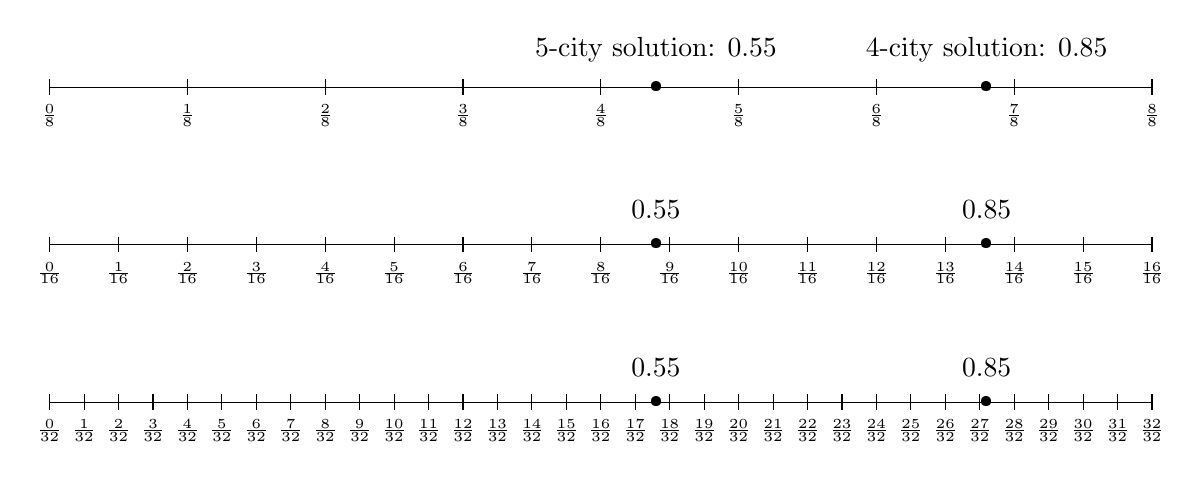
\begin{tikzpicture}
	\pgfmathsetmacro{\lineLength}{14}
	
	% First line - 1/8 steps
	%\node[label=above :{0.5}] at (0.5*\lineLength,0) {\textbullet};
	\node[label=above:{5-city solution: 0.55}] at (0.55*\lineLength,0) {\textbullet};
	\node[label=above:{4-city solution: 0.85}] at (0.85*\lineLength,0) {\textbullet};
	\draw (0,0) -- (\lineLength,0);
	\foreach \x in {0,1,...,8} { 
		\draw (\x/8*\lineLength ,0.1) -- (\x/8*\lineLength ,-0.1) node[below] {\tiny$\frac{\x}{8}$};
	}
	
	% Second line - 1/16 steps
	\node[label=above:{0.55}] at (0.55*\lineLength,-2) {\textbullet};
	\node[label=above:{0.85}] at (0.85*\lineLength,-2) {\textbullet};
	\draw (0,-2) -- (\lineLength,-2);
	\foreach \x in {0,1,...,16} { 
		\draw (\x/16*\lineLength,-1.9) -- (\x/16*\lineLength,-2.1) node[below] {\tiny$\frac{\x}{16}$};
	}
	
	% Third line - 1/32 steps
	\node[label=above:{0.55}] at (0.55*\lineLength,-4) {\textbullet};
	\node[label=above:{0.85}] at (0.85*\lineLength,-4) {\textbullet};
	\draw (0,-4) -- (\lineLength,-4);
	\foreach \x in {0,1,...,32} {
		\draw (\x/32*\lineLength,-3.9) -- (\x/32*\lineLength,-4.1) node[below] {\tiny$\frac{\x}{32}$};
	}
	
\end{tikzpicture}
	
	An easy way to interpret the number lines is that when the value is close to a specific step, that step is more likely to be measured. If it is perfectly inbetween two steps, we get the best possible approximation is either the lower bound or the upper bound both with the exact same probability, $P_b \approx 40\%$. It is important to note, that we are measuring two independent phases for each hamiltonian cycle, thus our best approximation will be $P_b^2 \approx 16\%$. 
	
	We can see for the 4-qubit estimation, the introduction of a more precise value of $13/16$ increased its probability of being measured as a good approximation for $0.85$ and in turn decreased the probabiliy of $7/8  = 14/16$ being measured. Performing 5-qubit estimation does improve our results but does not justify the computational cost considering we achieved similiar results with 3-qubit estimation. We see a similiar issue with our results for the 5-city problem, we only simulated 3 and 4-qubit estimation but had we done 5, our confidence in the result would have decreased.
	
	Unless we obtain a fortunate solution as in cycle 8 of the 5-city problem (FIG. \ref{fig:5-city-7-9}), where our phase ($0.5$) can be respresented exactly, we need to run phase estimation a number of times from which we can use the mode of our results as the solution. And as we've discussed earlier, using a larger number of phase qubits does not neccesarily improve your confidence in the result. If we only consider the states with the highest counts in Tables \ref{table:sim-results-4-city},  \ref{table:sim-results-4-city}, then our results perfectly predict the solutions and non-solutions.
	
	The question we need to ask is now is how many phase qubits are needed correctly identify a solution or non-solution based on the most frequent state measured? And the answer is we need to make sure the resolution of our phase qubits is larger than the constraint value, $\alpha$, of the problem (Eq. \ref{constraint-alpha}). Lets consider a non-solution where the reduction to the phase is exactly the resolution of 3-qubit estimation, 0.125:
	
	
	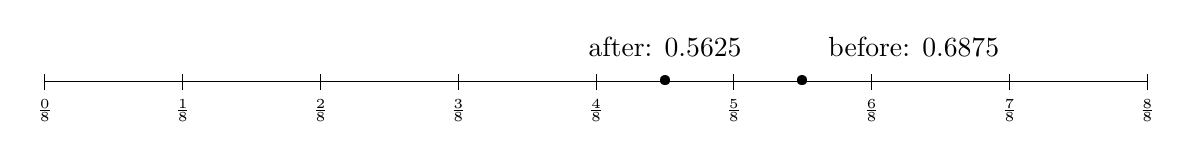
\begin{tikzpicture}
		\pgfmathsetmacro{\lineLength}{14}
		
		% First line - 1/8 steps
		%\node[label=above :{0.5}] at (0.5*\lineLength,0) {\textbullet};
		\node[label=above:{after: 0.5625}] at (0.5625*\lineLength,0) {\textbullet};
		\node[label=above right :{before: 0.6875}] at (0.6875*\lineLength,0) {\textbullet};
		\draw (0,0) -- (\lineLength,0);
		\foreach \x in {0,1,...,8} { 
			\draw (\x/8*\lineLength ,0.1) -- (\x/8*\lineLength ,-0.1) node[below] {\tiny$\frac{\x}{8}$};
		}
	\end{tikzpicture}
	
	
	Based on our best approximation, we are likely to obtain any of the four following results most frequently with $P^2_b  \approx 16\%$:

	$$P_1: 0.625, 0.625$$
	$$P_2: 0.500, 0.625$$
	$$P_3: 0.625, 0.750$$
	$$P_4: 0.500, 0.750$$
	
	Here we can see we run a risk of selecting $P_1$. By extending the distance between our phases, we reduce the probability of measuring $0.625$ and we can qualitatively predict how probable our four results above will be:
	
		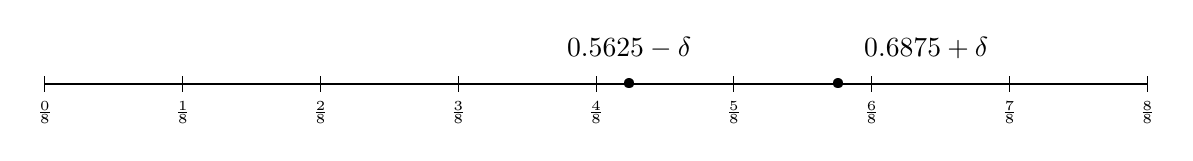
\begin{tikzpicture}
		\pgfmathsetmacro{\lineLength}{14}
		
		% First line - 1/8 steps
		%\node[label=above :{0.5}] at (0.5*\lineLength,0) {\textbullet};
		\node[label=above:{$0.5625-\delta$}] at (0.53*\lineLength,0) {\textbullet};
		\node[label=above right :{$0.6875 + \delta$}] at (0.72*\lineLength,0) {\textbullet};
		\draw (0,0) -- (\lineLength,0);
		\foreach \x in {0,1,...,8} { 
			\draw (\x/8*\lineLength ,0.1) -- (\x/8*\lineLength ,-0.1) node[below] {\tiny$\frac{\x}{8}$};
		}
	\end{tikzpicture}
	
 $$P_1 < P_2 = P_3 < P_4$$
 
 We actually simulated a similiar case in cycle 7 of our 5-city problem (FIG. \ref{fig:5-city-7-9}), where the least probable result of the top 4 states, indicated the cycle was a solution.  If $\delta << 1$, we would have to run our circuit many times over to appropriately measure the non-solution as the most frequent result. Otherwise we run the risk again of predicting a solution with $P_1$ as it would be very close to $P_4$. A safe bet would be to have a phase resolution atleast twice the constraint value. Lets illustrate this again by inconveniently placing the phases we hope to estimate perfecly inbetween steps:
 
 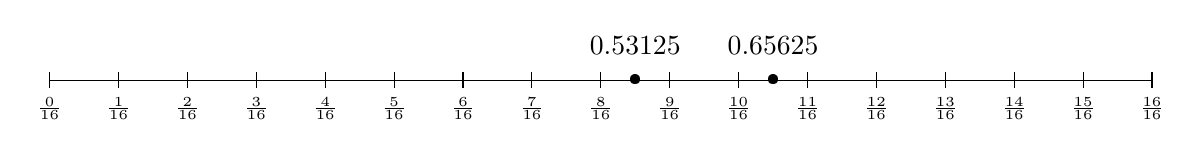
\begin{tikzpicture}
 	\pgfmathsetmacro{\lineLength}{14}
 	
	% Second line - 1/16 steps
\node[label=above:{0.53125}] at (0.53125*\lineLength,-2) {\textbullet};
\node[label=above:{0.65625}] at (0.65625*\lineLength,-2) {\textbullet};
\draw (0,-2) -- (\lineLength,-2);
\foreach \x in {0,1,...,16} { 
	\draw (\x/16*\lineLength,-1.9) -- (\x/16*\lineLength,-2.1) node[below] {\tiny$\frac{\x}{16}$};
}
 \end{tikzpicture}
 
 We now run zero risk of the four most probable states indicating a solution. As our measurement will likely collapse to any of these four options with $P^2_b  \approx 16\%$:
 
 $$P_1: 0.5000, 0.6250$$
 $$P_2: 0.5000, 0.6875$$
 $$P_3: 0.5625, 0.6250$$
 $$P_4: 0.5625, 0.6875$$
 
And we can also show in the case of a solution, two of the four states will show it is a solution and the other two will not, but we can confidently say it is simply a rounding error since our constraint value would reduce a phase by much more. We can illustrate this considering the phase $0.65625$:


 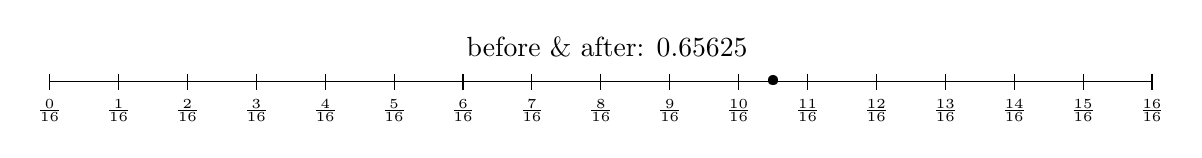
\begin{tikzpicture}
	\pgfmathsetmacro{\lineLength}{14}
	
	% Second line - 1/16 steps
	\node[label=above left :{before \& after: 0.65625}] at (0.65625*\lineLength,-2) {\textbullet};
	\draw (0,-2) -- (\lineLength,-2);
	\foreach \x in {0,1,...,16} { 
		\draw (\x/16*\lineLength,-1.9) -- (\x/16*\lineLength,-2.1) node[below] {\tiny$\frac{\x}{16}$};
	}
\end{tikzpicture}

$$P_1: 0.6250, 0.6250$$
$$P_2: 0.6250, 0.6875$$
$$P_3: 0.6875, 0.6250$$
$$P_4: 0.6875, 0.6875$$


We can also discuss the number of eigenstate qubits needed. Our method asks us to construct a matrix of size $N^N \times N^N$, where $N$ represents the number of cities. This does result in a unitary matrix however, it cannot be neccesarily represented by an exact number of qubits.We saw this issue in our 5-city problem, where we introduced ones at the end of the matrix (Eq.\ref{ones}). If $n$ represents the number of qubits we need and $m$ represents the number of cities, we need to solve the equation:

$$2^n = m^m$$
$$n = m\mathrm{log}_2(m)$$

With this we can conclude the number of eigenstate qubits needed will scale polynomially where it $<m^2$. For example in the case of 5 cities, $n \approx 11.6$ and we round up to $12$ qubits. 

Because we run through all hamiltonian cycles to solve this problem our time complexity remains $O((N-1)!)$. We can however solve this decision problem by running all hamiltonian cycles in parallel reducing our  execution time but the tradeoff would be introducing exponential space complexity, $O((N-1)!)$ .
	
	\bibliographystyle{unsrt}
	%\bibliography{references,refs}
	\bibliography{ref}
	%\printbibliography  %[heading=none, keyword=OWN]
	%% Use this to reset the appendix counter.  Note that the FoGS
	%% requires that the word ``Appendices'' appear in the table of
	%% contents either before each appendix lable or as a division
	%% denoting the start of the appendices.  We take the latter option
	%% here.  This is ensured by making the \texttt{appendicestoc} option
	%% a default option to the UBC thesis class.
	
	%%% If you only have one appendix, please uncomment the following line.
	% \renewcommand{\appendicesname}{Appendix}
	\appendix
	\chapter{Hamiltonian Cycles and Locating Eigenstates Code}
	
	The code detailed in this section can be used to generate the information found in Tables \ref{table:ham-cycle-details-4-city}, \ref{table:4-city-conversions},  \ref{table:ham-cycle-details-5-city} and \ref{table:5-city-conversions}, which construct the Hamiltonian cycles and locate the eigenstates. 
	
	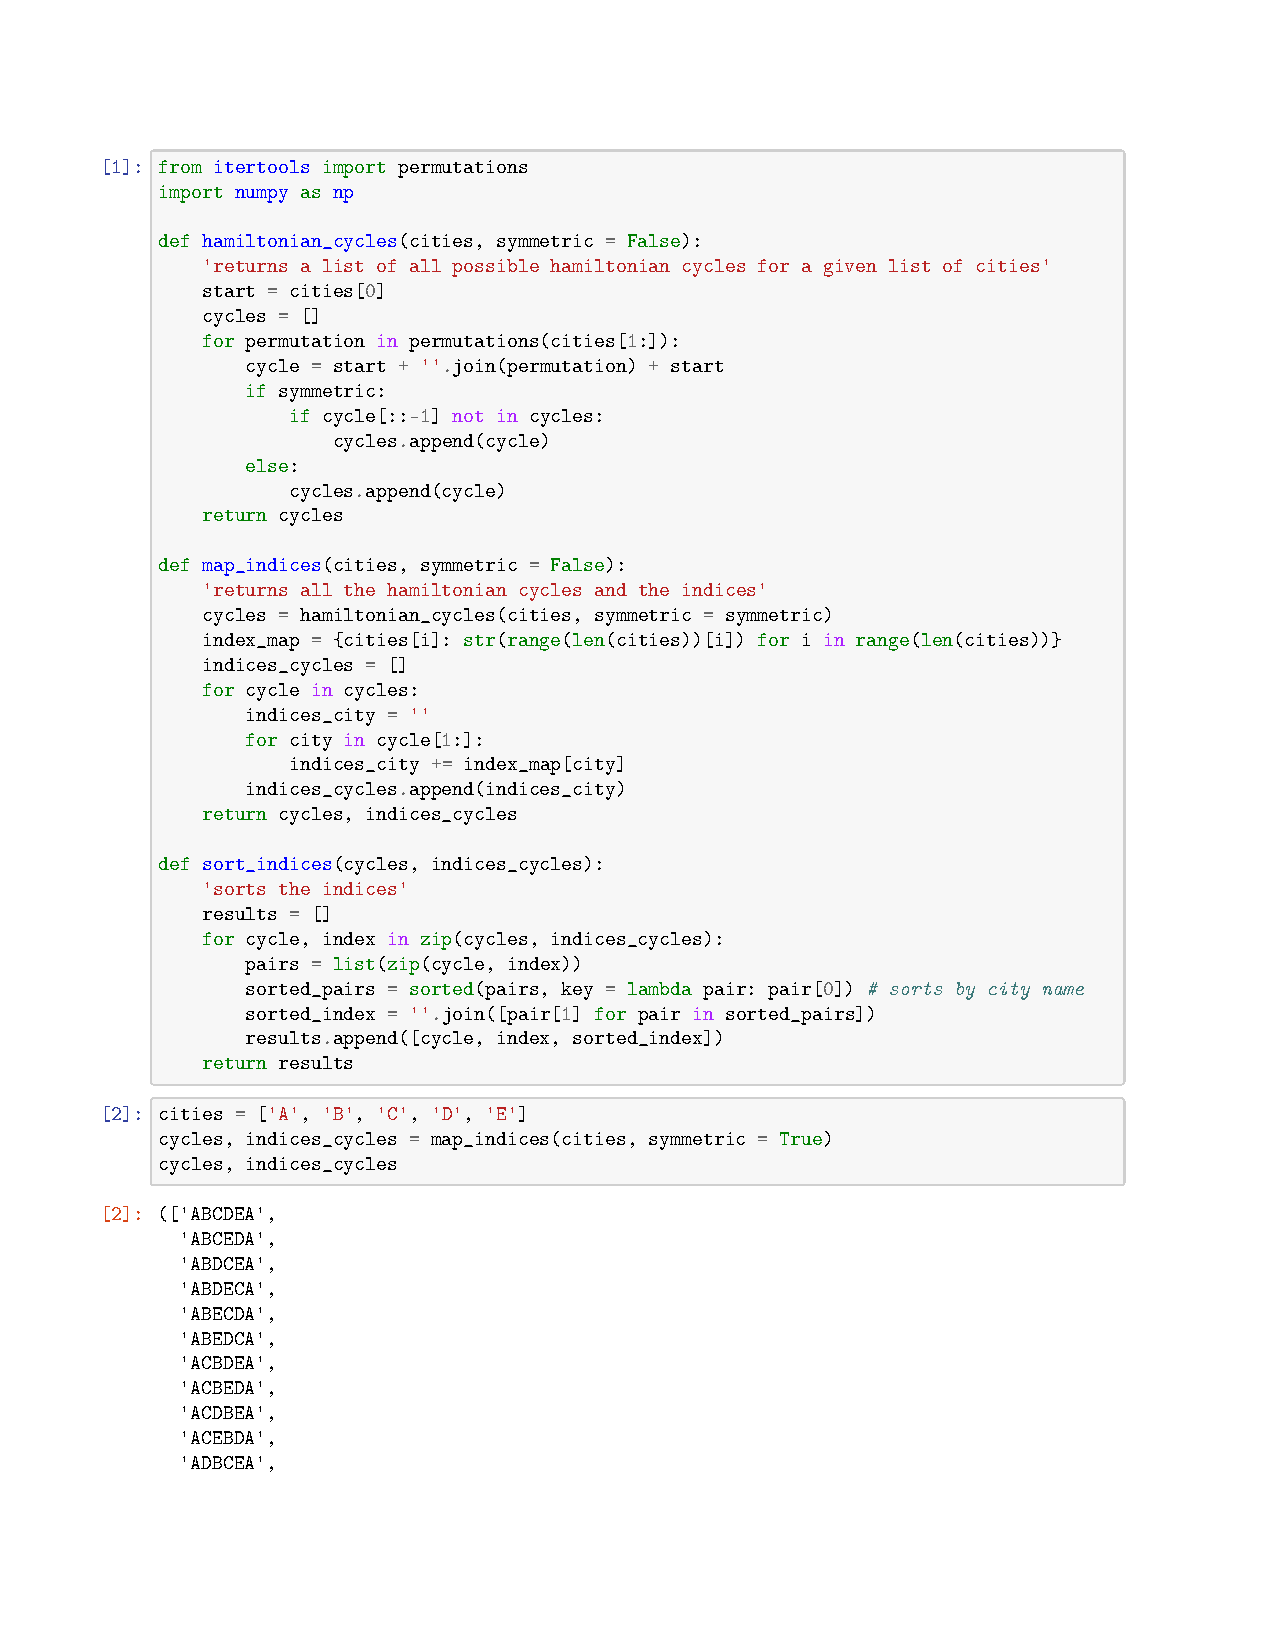
\includepdf[pages=-]{hamiltonian_cycles.pdf}
	%\input{ham_cycles.tex}
	%\documentclass[15pt]{article}

    \usepackage[breakable]{tcolorbox}
    \usepackage{parskip} % Stop auto-indenting (to mimic markdown behaviour)
    

    % Basic figure setup, for now with no caption control since it's done
    % automatically by Pandoc (which extracts ![](path) syntax from Markdown).
    \usepackage{graphicx}
    % Maintain compatibility with old templates. Remove in nbconvert 6.0
    \let\Oldincludegraphics\includegraphics
    % Ensure that by default, figures have no caption (until we provide a
    % proper Figure object with a Caption API and a way to capture that
    % in the conversion process - todo).
    \usepackage{caption}
    \DeclareCaptionFormat{nocaption}{}
    \captionsetup{format=nocaption,aboveskip=0pt,belowskip=0pt}

    \usepackage{float}
    \floatplacement{figure}{H} % forces figures to be placed at the correct location
    \usepackage{xcolor} % Allow colors to be defined
    \usepackage{enumerate} % Needed for markdown enumerations to work
    \usepackage{geometry} % Used to adjust the document margins
    \usepackage{amsmath} % Equations
    \usepackage{amssymb} % Equations
    \usepackage{textcomp} % defines textquotesingle
    % Hack from http://tex.stackexchange.com/a/47451/13684:
    \AtBeginDocument{%
        \def\PYZsq{\textquotesingle}% Upright quotes in Pygmentized code
    }
    \usepackage{upquote} % Upright quotes for verbatim code
    \usepackage{eurosym} % defines \euro

    \usepackage{iftex}
    \ifPDFTeX
        \usepackage[T1]{fontenc}
        \IfFileExists{alphabeta.sty}{
              \usepackage{alphabeta}
          }{
              \usepackage[mathletters]{ucs}
              \usepackage[utf8x]{inputenc}
          }
    \else
        \usepackage{fontspec}
        \usepackage{unicode-math}
    \fi

    \usepackage{fancyvrb} % verbatim replacement that allows latex
    \usepackage{grffile} % extends the file name processing of package graphics
                         % to support a larger range
    \makeatletter % fix for old versions of grffile with XeLaTeX
    \@ifpackagelater{grffile}{2019/11/01}
    {
      % Do nothing on new versions
    }
    {
      \def\Gread@@xetex#1{%
        \IfFileExists{"\Gin@base".bb}%
        {\Gread@eps{\Gin@base.bb}}%
        {\Gread@@xetex@aux#1}%
      }
    }
    \makeatother
    \usepackage[Export]{adjustbox} % Used to constrain images to a maximum size
    \adjustboxset{max size={0.9\linewidth}{0.9\paperheight}}

    % The hyperref package gives us a pdf with properly built
    % internal navigation ('pdf bookmarks' for the table of contents,
    % internal cross-reference links, web links for URLs, etc.)
    \usepackage{hyperref}
    % The default LaTeX title has an obnoxious amount of whitespace. By default,
    % titling removes some of it. It also provides customization options.
    \usepackage{titling}
    \usepackage{longtable} % longtable support required by pandoc >1.10
    \usepackage{booktabs}  % table support for pandoc > 1.12.2
    \usepackage{array}     % table support for pandoc >= 2.11.3
    \usepackage{calc}      % table minipage width calculation for pandoc >= 2.11.1
    \usepackage[inline]{enumitem} % IRkernel/repr support (it uses the enumerate* environment)
    \usepackage[normalem]{ulem} % ulem is needed to support strikethroughs (\sout)
                                % normalem makes italics be italics, not underlines
    \usepackage{mathrsfs}
    

    
    % Colors for the hyperref package
    \definecolor{urlcolor}{rgb}{0,.145,.698}
    \definecolor{linkcolor}{rgb}{.71,0.21,0.01}
    \definecolor{citecolor}{rgb}{.12,.54,.11}

    % ANSI colors
    \definecolor{ansi-black}{HTML}{3E424D}
    \definecolor{ansi-black-intense}{HTML}{282C36}
    \definecolor{ansi-red}{HTML}{E75C58}
    \definecolor{ansi-red-intense}{HTML}{B22B31}
    \definecolor{ansi-green}{HTML}{00A250}
    \definecolor{ansi-green-intense}{HTML}{007427}
    \definecolor{ansi-yellow}{HTML}{DDB62B}
    \definecolor{ansi-yellow-intense}{HTML}{B27D12}
    \definecolor{ansi-blue}{HTML}{208FFB}
    \definecolor{ansi-blue-intense}{HTML}{0065CA}
    \definecolor{ansi-magenta}{HTML}{D160C4}
    \definecolor{ansi-magenta-intense}{HTML}{A03196}
    \definecolor{ansi-cyan}{HTML}{60C6C8}
    \definecolor{ansi-cyan-intense}{HTML}{258F8F}
    \definecolor{ansi-white}{HTML}{C5C1B4}
    \definecolor{ansi-white-intense}{HTML}{A1A6B2}
    \definecolor{ansi-default-inverse-fg}{HTML}{FFFFFF}
    \definecolor{ansi-default-inverse-bg}{HTML}{000000}

    % common color for the border for error outputs.
    \definecolor{outerrorbackground}{HTML}{FFDFDF}

    % commands and environments needed by pandoc snippets
    % extracted from the output of `pandoc -s`
    \providecommand{\tightlist}{%
      \setlength{\itemsep}{0pt}\setlength{\parskip}{0pt}}
    \DefineVerbatimEnvironment{Highlighting}{Verbatim}{commandchars=\\\{\}}
    % Add ',fontsize=\small' for more characters per line
    \newenvironment{Shaded}{}{}
    \newcommand{\KeywordTok}[1]{\textcolor[rgb]{0.00,0.44,0.13}{\textbf{{#1}}}}
    \newcommand{\DataTypeTok}[1]{\textcolor[rgb]{0.56,0.13,0.00}{{#1}}}
    \newcommand{\DecValTok}[1]{\textcolor[rgb]{0.25,0.63,0.44}{{#1}}}
    \newcommand{\BaseNTok}[1]{\textcolor[rgb]{0.25,0.63,0.44}{{#1}}}
    \newcommand{\FloatTok}[1]{\textcolor[rgb]{0.25,0.63,0.44}{{#1}}}
    \newcommand{\CharTok}[1]{\textcolor[rgb]{0.25,0.44,0.63}{{#1}}}
    \newcommand{\StringTok}[1]{\textcolor[rgb]{0.25,0.44,0.63}{{#1}}}
    \newcommand{\CommentTok}[1]{\textcolor[rgb]{0.38,0.63,0.69}{\textit{{#1}}}}
    \newcommand{\OtherTok}[1]{\textcolor[rgb]{0.00,0.44,0.13}{{#1}}}
    \newcommand{\AlertTok}[1]{\textcolor[rgb]{1.00,0.00,0.00}{\textbf{{#1}}}}
    \newcommand{\FunctionTok}[1]{\textcolor[rgb]{0.02,0.16,0.49}{{#1}}}
    \newcommand{\RegionMarkerTok}[1]{{#1}}
    \newcommand{\ErrorTok}[1]{\textcolor[rgb]{1.00,0.00,0.00}{\textbf{{#1}}}}
    \newcommand{\NormalTok}[1]{{#1}}

    % Additional commands for more recent versions of Pandoc
    \newcommand{\ConstantTok}[1]{\textcolor[rgb]{0.53,0.00,0.00}{{#1}}}
    \newcommand{\SpecialCharTok}[1]{\textcolor[rgb]{0.25,0.44,0.63}{{#1}}}
    \newcommand{\VerbatimStringTok}[1]{\textcolor[rgb]{0.25,0.44,0.63}{{#1}}}
    \newcommand{\SpecialStringTok}[1]{\textcolor[rgb]{0.73,0.40,0.53}{{#1}}}
    \newcommand{\ImportTok}[1]{{#1}}
    \newcommand{\DocumentationTok}[1]{\textcolor[rgb]{0.73,0.13,0.13}{\textit{{#1}}}}
    \newcommand{\AnnotationTok}[1]{\textcolor[rgb]{0.38,0.63,0.69}{\textbf{\textit{{#1}}}}}
    \newcommand{\CommentVarTok}[1]{\textcolor[rgb]{0.38,0.63,0.69}{\textbf{\textit{{#1}}}}}
    \newcommand{\VariableTok}[1]{\textcolor[rgb]{0.10,0.09,0.49}{{#1}}}
    \newcommand{\ControlFlowTok}[1]{\textcolor[rgb]{0.00,0.44,0.13}{\textbf{{#1}}}}
    \newcommand{\OperatorTok}[1]{\textcolor[rgb]{0.40,0.40,0.40}{{#1}}}
    \newcommand{\BuiltInTok}[1]{{#1}}
    \newcommand{\ExtensionTok}[1]{{#1}}
    \newcommand{\PreprocessorTok}[1]{\textcolor[rgb]{0.74,0.48,0.00}{{#1}}}
    \newcommand{\AttributeTok}[1]{\textcolor[rgb]{0.49,0.56,0.16}{{#1}}}
    \newcommand{\InformationTok}[1]{\textcolor[rgb]{0.38,0.63,0.69}{\textbf{\textit{{#1}}}}}
    \newcommand{\WarningTok}[1]{\textcolor[rgb]{0.38,0.63,0.69}{\textbf{\textit{{#1}}}}}


    % Define a nice break command that doesn't care if a line doesn't already
    % exist.
    \def\br{\hspace*{\fill} \\* }
    % Math Jax compatibility definitions
    \def\gt{>}
    \def\lt{<}
    \let\Oldtex\TeX
    \let\Oldlatex\LaTeX
    \renewcommand{\TeX}{\textrm{\Oldtex}}
    \renewcommand{\LaTeX}{\textrm{\Oldlatex}}
    % Document parameters
    % Document title
    \title{hamiltonian\_cycles}
    
    
    
    
    
% Pygments definitions
\makeatletter
\def\PY@reset{\let\PY@it=\relax \let\PY@bf=\relax%
    \let\PY@ul=\relax \let\PY@tc=\relax%
    \let\PY@bc=\relax \let\PY@ff=\relax}
\def\PY@tok#1{\csname PY@tok@#1\endcsname}
\def\PY@toks#1+{\ifx\relax#1\empty\else%
    \PY@tok{#1}\expandafter\PY@toks\fi}
\def\PY@do#1{\PY@bc{\PY@tc{\PY@ul{%
    \PY@it{\PY@bf{\PY@ff{#1}}}}}}}
\def\PY#1#2{\PY@reset\PY@toks#1+\relax+\PY@do{#2}}

\@namedef{PY@tok@w}{\def\PY@tc##1{\textcolor[rgb]{0.73,0.73,0.73}{##1}}}
\@namedef{PY@tok@c}{\let\PY@it=\textit\def\PY@tc##1{\textcolor[rgb]{0.24,0.48,0.48}{##1}}}
\@namedef{PY@tok@cp}{\def\PY@tc##1{\textcolor[rgb]{0.61,0.40,0.00}{##1}}}
\@namedef{PY@tok@k}{\let\PY@bf=\textbf\def\PY@tc##1{\textcolor[rgb]{0.00,0.50,0.00}{##1}}}
\@namedef{PY@tok@kp}{\def\PY@tc##1{\textcolor[rgb]{0.00,0.50,0.00}{##1}}}
\@namedef{PY@tok@kt}{\def\PY@tc##1{\textcolor[rgb]{0.69,0.00,0.25}{##1}}}
\@namedef{PY@tok@o}{\def\PY@tc##1{\textcolor[rgb]{0.40,0.40,0.40}{##1}}}
\@namedef{PY@tok@ow}{\let\PY@bf=\textbf\def\PY@tc##1{\textcolor[rgb]{0.67,0.13,1.00}{##1}}}
\@namedef{PY@tok@nb}{\def\PY@tc##1{\textcolor[rgb]{0.00,0.50,0.00}{##1}}}
\@namedef{PY@tok@nf}{\def\PY@tc##1{\textcolor[rgb]{0.00,0.00,1.00}{##1}}}
\@namedef{PY@tok@nc}{\let\PY@bf=\textbf\def\PY@tc##1{\textcolor[rgb]{0.00,0.00,1.00}{##1}}}
\@namedef{PY@tok@nn}{\let\PY@bf=\textbf\def\PY@tc##1{\textcolor[rgb]{0.00,0.00,1.00}{##1}}}
\@namedef{PY@tok@ne}{\let\PY@bf=\textbf\def\PY@tc##1{\textcolor[rgb]{0.80,0.25,0.22}{##1}}}
\@namedef{PY@tok@nv}{\def\PY@tc##1{\textcolor[rgb]{0.10,0.09,0.49}{##1}}}
\@namedef{PY@tok@no}{\def\PY@tc##1{\textcolor[rgb]{0.53,0.00,0.00}{##1}}}
\@namedef{PY@tok@nl}{\def\PY@tc##1{\textcolor[rgb]{0.46,0.46,0.00}{##1}}}
\@namedef{PY@tok@ni}{\let\PY@bf=\textbf\def\PY@tc##1{\textcolor[rgb]{0.44,0.44,0.44}{##1}}}
\@namedef{PY@tok@na}{\def\PY@tc##1{\textcolor[rgb]{0.41,0.47,0.13}{##1}}}
\@namedef{PY@tok@nt}{\let\PY@bf=\textbf\def\PY@tc##1{\textcolor[rgb]{0.00,0.50,0.00}{##1}}}
\@namedef{PY@tok@nd}{\def\PY@tc##1{\textcolor[rgb]{0.67,0.13,1.00}{##1}}}
\@namedef{PY@tok@s}{\def\PY@tc##1{\textcolor[rgb]{0.73,0.13,0.13}{##1}}}
\@namedef{PY@tok@sd}{\let\PY@it=\textit\def\PY@tc##1{\textcolor[rgb]{0.73,0.13,0.13}{##1}}}
\@namedef{PY@tok@si}{\let\PY@bf=\textbf\def\PY@tc##1{\textcolor[rgb]{0.64,0.35,0.47}{##1}}}
\@namedef{PY@tok@se}{\let\PY@bf=\textbf\def\PY@tc##1{\textcolor[rgb]{0.67,0.36,0.12}{##1}}}
\@namedef{PY@tok@sr}{\def\PY@tc##1{\textcolor[rgb]{0.64,0.35,0.47}{##1}}}
\@namedef{PY@tok@ss}{\def\PY@tc##1{\textcolor[rgb]{0.10,0.09,0.49}{##1}}}
\@namedef{PY@tok@sx}{\def\PY@tc##1{\textcolor[rgb]{0.00,0.50,0.00}{##1}}}
\@namedef{PY@tok@m}{\def\PY@tc##1{\textcolor[rgb]{0.40,0.40,0.40}{##1}}}
\@namedef{PY@tok@gh}{\let\PY@bf=\textbf\def\PY@tc##1{\textcolor[rgb]{0.00,0.00,0.50}{##1}}}
\@namedef{PY@tok@gu}{\let\PY@bf=\textbf\def\PY@tc##1{\textcolor[rgb]{0.50,0.00,0.50}{##1}}}
\@namedef{PY@tok@gd}{\def\PY@tc##1{\textcolor[rgb]{0.63,0.00,0.00}{##1}}}
\@namedef{PY@tok@gi}{\def\PY@tc##1{\textcolor[rgb]{0.00,0.52,0.00}{##1}}}
\@namedef{PY@tok@gr}{\def\PY@tc##1{\textcolor[rgb]{0.89,0.00,0.00}{##1}}}
\@namedef{PY@tok@ge}{\let\PY@it=\textit}
\@namedef{PY@tok@gs}{\let\PY@bf=\textbf}
\@namedef{PY@tok@gp}{\let\PY@bf=\textbf\def\PY@tc##1{\textcolor[rgb]{0.00,0.00,0.50}{##1}}}
\@namedef{PY@tok@go}{\def\PY@tc##1{\textcolor[rgb]{0.44,0.44,0.44}{##1}}}
\@namedef{PY@tok@gt}{\def\PY@tc##1{\textcolor[rgb]{0.00,0.27,0.87}{##1}}}
\@namedef{PY@tok@err}{\def\PY@bc##1{{\setlength{\fboxsep}{\string -\fboxrule}\fcolorbox[rgb]{1.00,0.00,0.00}{1,1,1}{\strut ##1}}}}
\@namedef{PY@tok@kc}{\let\PY@bf=\textbf\def\PY@tc##1{\textcolor[rgb]{0.00,0.50,0.00}{##1}}}
\@namedef{PY@tok@kd}{\let\PY@bf=\textbf\def\PY@tc##1{\textcolor[rgb]{0.00,0.50,0.00}{##1}}}
\@namedef{PY@tok@kn}{\let\PY@bf=\textbf\def\PY@tc##1{\textcolor[rgb]{0.00,0.50,0.00}{##1}}}
\@namedef{PY@tok@kr}{\let\PY@bf=\textbf\def\PY@tc##1{\textcolor[rgb]{0.00,0.50,0.00}{##1}}}
\@namedef{PY@tok@bp}{\def\PY@tc##1{\textcolor[rgb]{0.00,0.50,0.00}{##1}}}
\@namedef{PY@tok@fm}{\def\PY@tc##1{\textcolor[rgb]{0.00,0.00,1.00}{##1}}}
\@namedef{PY@tok@vc}{\def\PY@tc##1{\textcolor[rgb]{0.10,0.09,0.49}{##1}}}
\@namedef{PY@tok@vg}{\def\PY@tc##1{\textcolor[rgb]{0.10,0.09,0.49}{##1}}}
\@namedef{PY@tok@vi}{\def\PY@tc##1{\textcolor[rgb]{0.10,0.09,0.49}{##1}}}
\@namedef{PY@tok@vm}{\def\PY@tc##1{\textcolor[rgb]{0.10,0.09,0.49}{##1}}}
\@namedef{PY@tok@sa}{\def\PY@tc##1{\textcolor[rgb]{0.73,0.13,0.13}{##1}}}
\@namedef{PY@tok@sb}{\def\PY@tc##1{\textcolor[rgb]{0.73,0.13,0.13}{##1}}}
\@namedef{PY@tok@sc}{\def\PY@tc##1{\textcolor[rgb]{0.73,0.13,0.13}{##1}}}
\@namedef{PY@tok@dl}{\def\PY@tc##1{\textcolor[rgb]{0.73,0.13,0.13}{##1}}}
\@namedef{PY@tok@s2}{\def\PY@tc##1{\textcolor[rgb]{0.73,0.13,0.13}{##1}}}
\@namedef{PY@tok@sh}{\def\PY@tc##1{\textcolor[rgb]{0.73,0.13,0.13}{##1}}}
\@namedef{PY@tok@s1}{\def\PY@tc##1{\textcolor[rgb]{0.73,0.13,0.13}{##1}}}
\@namedef{PY@tok@mb}{\def\PY@tc##1{\textcolor[rgb]{0.40,0.40,0.40}{##1}}}
\@namedef{PY@tok@mf}{\def\PY@tc##1{\textcolor[rgb]{0.40,0.40,0.40}{##1}}}
\@namedef{PY@tok@mh}{\def\PY@tc##1{\textcolor[rgb]{0.40,0.40,0.40}{##1}}}
\@namedef{PY@tok@mi}{\def\PY@tc##1{\textcolor[rgb]{0.40,0.40,0.40}{##1}}}
\@namedef{PY@tok@il}{\def\PY@tc##1{\textcolor[rgb]{0.40,0.40,0.40}{##1}}}
\@namedef{PY@tok@mo}{\def\PY@tc##1{\textcolor[rgb]{0.40,0.40,0.40}{##1}}}
\@namedef{PY@tok@ch}{\let\PY@it=\textit\def\PY@tc##1{\textcolor[rgb]{0.24,0.48,0.48}{##1}}}
\@namedef{PY@tok@cm}{\let\PY@it=\textit\def\PY@tc##1{\textcolor[rgb]{0.24,0.48,0.48}{##1}}}
\@namedef{PY@tok@cpf}{\let\PY@it=\textit\def\PY@tc##1{\textcolor[rgb]{0.24,0.48,0.48}{##1}}}
\@namedef{PY@tok@c1}{\let\PY@it=\textit\def\PY@tc##1{\textcolor[rgb]{0.24,0.48,0.48}{##1}}}
\@namedef{PY@tok@cs}{\let\PY@it=\textit\def\PY@tc##1{\textcolor[rgb]{0.24,0.48,0.48}{##1}}}

\def\PYZbs{\char`\\}
\def\PYZus{\char`\_}
\def\PYZob{\char`\{}
\def\PYZcb{\char`\}}
\def\PYZca{\char`\^}
\def\PYZam{\char`\&}
\def\PYZlt{\char`\<}
\def\PYZgt{\char`\>}
\def\PYZsh{\char`\#}
\def\PYZpc{\char`\%}
\def\PYZdl{\char`\$}
\def\PYZhy{\char`\-}
\def\PYZsq{\char`\'}
\def\PYZdq{\char`\"}
\def\PYZti{\char`\~}
% for compatibility with earlier versions
\def\PYZat{@}
\def\PYZlb{[}
\def\PYZrb{]}
\makeatother


    % For linebreaks inside Verbatim environment from package fancyvrb.
    \makeatletter
        \newbox\Wrappedcontinuationbox
        \newbox\Wrappedvisiblespacebox
        \newcommand*\Wrappedvisiblespace {\textcolor{red}{\textvisiblespace}}
        \newcommand*\Wrappedcontinuationsymbol {\textcolor{red}{\llap{\tiny$\m@th\hookrightarrow$}}}
        \newcommand*\Wrappedcontinuationindent {3ex }
        \newcommand*\Wrappedafterbreak {\kern\Wrappedcontinuationindent\copy\Wrappedcontinuationbox}
        % Take advantage of the already applied Pygments mark-up to insert
        % potential linebreaks for TeX processing.
        %        {, <, #, %, $, ' and ": go to next line.
        %        _, }, ^, &, >, - and ~: stay at end of broken line.
        % Use of \textquotesingle for straight quote.
        \newcommand*\Wrappedbreaksatspecials {%
            \def\PYGZus{\discretionary{\char`\_}{\Wrappedafterbreak}{\char`\_}}%
            \def\PYGZob{\discretionary{}{\Wrappedafterbreak\char`\{}{\char`\{}}%
            \def\PYGZcb{\discretionary{\char`\}}{\Wrappedafterbreak}{\char`\}}}%
            \def\PYGZca{\discretionary{\char`\^}{\Wrappedafterbreak}{\char`\^}}%
            \def\PYGZam{\discretionary{\char`\&}{\Wrappedafterbreak}{\char`\&}}%
            \def\PYGZlt{\discretionary{}{\Wrappedafterbreak\char`\<}{\char`\<}}%
            \def\PYGZgt{\discretionary{\char`\>}{\Wrappedafterbreak}{\char`\>}}%
            \def\PYGZsh{\discretionary{}{\Wrappedafterbreak\char`\#}{\char`\#}}%
            \def\PYGZpc{\discretionary{}{\Wrappedafterbreak\char`\%}{\char`\%}}%
            \def\PYGZdl{\discretionary{}{\Wrappedafterbreak\char`\$}{\char`\$}}%
            \def\PYGZhy{\discretionary{\char`\-}{\Wrappedafterbreak}{\char`\-}}%
            \def\PYGZsq{\discretionary{}{\Wrappedafterbreak\textquotesingle}{\textquotesingle}}%
            \def\PYGZdq{\discretionary{}{\Wrappedafterbreak\char`\"}{\char`\"}}%
            \def\PYGZti{\discretionary{\char`\~}{\Wrappedafterbreak}{\char`\~}}%
        }
        % Some characters . , ; ? ! / are not pygmentized.
        % This macro makes them "active" and they will insert potential linebreaks
        \newcommand*\Wrappedbreaksatpunct {%
            \lccode`\~`\.\lowercase{\def~}{\discretionary{\hbox{\char`\.}}{\Wrappedafterbreak}{\hbox{\char`\.}}}%
            \lccode`\~`\,\lowercase{\def~}{\discretionary{\hbox{\char`\,}}{\Wrappedafterbreak}{\hbox{\char`\,}}}%
            \lccode`\~`\;\lowercase{\def~}{\discretionary{\hbox{\char`\;}}{\Wrappedafterbreak}{\hbox{\char`\;}}}%
            \lccode`\~`\:\lowercase{\def~}{\discretionary{\hbox{\char`\:}}{\Wrappedafterbreak}{\hbox{\char`\:}}}%
            \lccode`\~`\?\lowercase{\def~}{\discretionary{\hbox{\char`\?}}{\Wrappedafterbreak}{\hbox{\char`\?}}}%
            \lccode`\~`\!\lowercase{\def~}{\discretionary{\hbox{\char`\!}}{\Wrappedafterbreak}{\hbox{\char`\!}}}%
            \lccode`\~`\/\lowercase{\def~}{\discretionary{\hbox{\char`\/}}{\Wrappedafterbreak}{\hbox{\char`\/}}}%
            \catcode`\.\active
            \catcode`\,\active
            \catcode`\;\active
            \catcode`\:\active
            \catcode`\?\active
            \catcode`\!\active
            \catcode`\/\active
            \lccode`\~`\~
        }
    \makeatother

    \let\OriginalVerbatim=\Verbatim
    \makeatletter
    \renewcommand{\Verbatim}[1][1]{%
        %\parskip\z@skip
        \sbox\Wrappedcontinuationbox {\Wrappedcontinuationsymbol}%
        \sbox\Wrappedvisiblespacebox {\FV@SetupFont\Wrappedvisiblespace}%
        \def\FancyVerbFormatLine ##1{\hsize\linewidth
            \vtop{\raggedright\hyphenpenalty\z@\exhyphenpenalty\z@
                \doublehyphendemerits\z@\finalhyphendemerits\z@
                \strut ##1\strut}%
        }%
        % If the linebreak is at a space, the latter will be displayed as visible
        % space at end of first line, and a continuation symbol starts next line.
        % Stretch/shrink are however usually zero for typewriter font.
        \def\FV@Space {%
            \nobreak\hskip\z@ plus\fontdimen3\font minus\fontdimen4\font
            \discretionary{\copy\Wrappedvisiblespacebox}{\Wrappedafterbreak}
            {\kern\fontdimen2\font}%
        }%

        % Allow breaks at special characters using \PYG... macros.
        \Wrappedbreaksatspecials
        % Breaks at punctuation characters . , ; ? ! and / need catcode=\active
        \OriginalVerbatim[#1,codes*=\Wrappedbreaksatpunct]%
    }
    \makeatother

    % Exact colors from NB
    \definecolor{incolor}{HTML}{303F9F}
    \definecolor{outcolor}{HTML}{D84315}
    \definecolor{cellborder}{HTML}{CFCFCF}
    \definecolor{cellbackground}{HTML}{F7F7F7}

    % prompt
    \makeatletter
    \newcommand{\boxspacing}{\kern\kvtcb@left@rule\kern\kvtcb@boxsep}
    \makeatother
    \newcommand{\prompt}[4]{
        {\ttfamily\llap{{\color{#2}[#3]:\hspace{3pt}#4}}\vspace{-\baselineskip}}
    }
    

    
    % Prevent overflowing lines due to hard-to-break entities
    \sloppy
    % Setup hyperref package
    \hypersetup{
      breaklinks=true,  % so long urls are correctly broken across lines
      colorlinks=true,
      urlcolor=urlcolor,
      linkcolor=linkcolor,
      citecolor=citecolor,
      }
    % Slightly bigger margins than the latex defaults
    
    \geometry{verbose,tmargin=1in,bmargin=1in,lmargin=1in,rmargin=1in}
    
    
\pagenumbering{gobble}
\begin{document}
    
    %\maketitle
    
    

    
    \begin{tcolorbox}[breakable, size=fbox, boxrule=1pt, pad at break*=1mm,colback=cellbackground, colframe=cellborder]
\prompt{In}{incolor}{1}{\boxspacing}
\begin{Verbatim}[commandchars=\\\{\}]
\PY{k+kn}{from} \PY{n+nn}{itertools} \PY{k+kn}{import} \PY{n}{permutations}
\PY{k+kn}{import} \PY{n+nn}{numpy} \PY{k}{as} \PY{n+nn}{np}

\PY{k}{def} \PY{n+nf}{hamiltonian\PYZus{}cycles}\PY{p}{(}\PY{n}{cities}\PY{p}{,} \PY{n}{symmetric} \PY{o}{=} \PY{k+kc}{False}\PY{p}{)}\PY{p}{:}
    \PY{l+s+s1}{\PYZsq{}}\PY{l+s+s1}{returns a list of all possible hamiltonian cycles for a given list of cities}\PY{l+s+s1}{\PYZsq{}}
    \PY{n}{start} \PY{o}{=} \PY{n}{cities}\PY{p}{[}\PY{l+m+mi}{0}\PY{p}{]}
    \PY{n}{cycles} \PY{o}{=} \PY{p}{[}\PY{p}{]}
    \PY{k}{for} \PY{n}{permutation} \PY{o+ow}{in} \PY{n}{permutations}\PY{p}{(}\PY{n}{cities}\PY{p}{[}\PY{l+m+mi}{1}\PY{p}{:}\PY{p}{]}\PY{p}{)}\PY{p}{:}
        \PY{n}{cycle} \PY{o}{=} \PY{n}{start} \PY{o}{+} \PY{l+s+s1}{\PYZsq{}}\PY{l+s+s1}{\PYZsq{}}\PY{o}{.}\PY{n}{join}\PY{p}{(}\PY{n}{permutation}\PY{p}{)} \PY{o}{+} \PY{n}{start}
        \PY{k}{if} \PY{n}{symmetric}\PY{p}{:}
            \PY{k}{if} \PY{n}{cycle}\PY{p}{[}\PY{p}{:}\PY{p}{:}\PY{o}{\PYZhy{}}\PY{l+m+mi}{1}\PY{p}{]} \PY{o+ow}{not} \PY{o+ow}{in} \PY{n}{cycles}\PY{p}{:}
                \PY{n}{cycles}\PY{o}{.}\PY{n}{append}\PY{p}{(}\PY{n}{cycle}\PY{p}{)}
        \PY{k}{else}\PY{p}{:}
            \PY{n}{cycles}\PY{o}{.}\PY{n}{append}\PY{p}{(}\PY{n}{cycle}\PY{p}{)}
    \PY{k}{return} \PY{n}{cycles}

\PY{k}{def} \PY{n+nf}{map\PYZus{}indices}\PY{p}{(}\PY{n}{cities}\PY{p}{,} \PY{n}{symmetric} \PY{o}{=} \PY{k+kc}{False}\PY{p}{)}\PY{p}{:}
    \PY{l+s+s1}{\PYZsq{}}\PY{l+s+s1}{returns all the hamiltonian cycles and the indices}\PY{l+s+s1}{\PYZsq{}}
    \PY{n}{cycles} \PY{o}{=} \PY{n}{hamiltonian\PYZus{}cycles}\PY{p}{(}\PY{n}{cities}\PY{p}{,} \PY{n}{symmetric} \PY{o}{=} \PY{n}{symmetric}\PY{p}{)}
    \PY{n}{index\PYZus{}map} \PY{o}{=} \PY{p}{\PYZob{}}\PY{n}{cities}\PY{p}{[}\PY{n}{i}\PY{p}{]}\PY{p}{:} \PY{n+nb}{str}\PY{p}{(}\PY{n+nb}{range}\PY{p}{(}\PY{n+nb}{len}\PY{p}{(}\PY{n}{cities}\PY{p}{)}\PY{p}{)}\PY{p}{[}\PY{n}{i}\PY{p}{]}\PY{p}{)} \PY{k}{for} \PY{n}{i} \PY{o+ow}{in} \PY{n+nb}{range}\PY{p}{(}\PY{n+nb}{len}\PY{p}{(}\PY{n}{cities}\PY{p}{)}\PY{p}{)}\PY{p}{\PYZcb{}}
    \PY{n}{indices\PYZus{}cycles} \PY{o}{=} \PY{p}{[}\PY{p}{]}
    \PY{k}{for} \PY{n}{cycle} \PY{o+ow}{in} \PY{n}{cycles}\PY{p}{:}
        \PY{n}{indices\PYZus{}city} \PY{o}{=} \PY{l+s+s1}{\PYZsq{}}\PY{l+s+s1}{\PYZsq{}}
        \PY{k}{for} \PY{n}{city} \PY{o+ow}{in} \PY{n}{cycle}\PY{p}{[}\PY{l+m+mi}{1}\PY{p}{:}\PY{p}{]}\PY{p}{:}
            \PY{n}{indices\PYZus{}city} \PY{o}{+}\PY{o}{=} \PY{n}{index\PYZus{}map}\PY{p}{[}\PY{n}{city}\PY{p}{]}    
        \PY{n}{indices\PYZus{}cycles}\PY{o}{.}\PY{n}{append}\PY{p}{(}\PY{n}{indices\PYZus{}city}\PY{p}{)}
    \PY{k}{return} \PY{n}{cycles}\PY{p}{,} \PY{n}{indices\PYZus{}cycles}  

\PY{k}{def} \PY{n+nf}{sort\PYZus{}indices}\PY{p}{(}\PY{n}{cycles}\PY{p}{,} \PY{n}{indices\PYZus{}cycles}\PY{p}{)}\PY{p}{:}
    \PY{l+s+s1}{\PYZsq{}}\PY{l+s+s1}{sorts the indices}\PY{l+s+s1}{\PYZsq{}}
    \PY{n}{results} \PY{o}{=} \PY{p}{[}\PY{p}{]}
    \PY{k}{for} \PY{n}{cycle}\PY{p}{,} \PY{n}{index} \PY{o+ow}{in} \PY{n+nb}{zip}\PY{p}{(}\PY{n}{cycles}\PY{p}{,} \PY{n}{indices\PYZus{}cycles}\PY{p}{)}\PY{p}{:}
        \PY{n}{pairs} \PY{o}{=} \PY{n+nb}{list}\PY{p}{(}\PY{n+nb}{zip}\PY{p}{(}\PY{n}{cycle}\PY{p}{,} \PY{n}{index}\PY{p}{)}\PY{p}{)} 
        \PY{n}{sorted\PYZus{}pairs} \PY{o}{=} \PY{n+nb}{sorted}\PY{p}{(}\PY{n}{pairs}\PY{p}{,} \PY{n}{key} \PY{o}{=} \PY{k}{lambda} \PY{n}{pair}\PY{p}{:} \PY{n}{pair}\PY{p}{[}\PY{l+m+mi}{0}\PY{p}{]}\PY{p}{)} \PY{c+c1}{\PYZsh{} sorts by city name}
        \PY{n}{sorted\PYZus{}index} \PY{o}{=} \PY{l+s+s1}{\PYZsq{}}\PY{l+s+s1}{\PYZsq{}}\PY{o}{.}\PY{n}{join}\PY{p}{(}\PY{p}{[}\PY{n}{pair}\PY{p}{[}\PY{l+m+mi}{1}\PY{p}{]} \PY{k}{for} \PY{n}{pair} \PY{o+ow}{in} \PY{n}{sorted\PYZus{}pairs}\PY{p}{]}\PY{p}{)}
        \PY{n}{results}\PY{o}{.}\PY{n}{append}\PY{p}{(}\PY{p}{[}\PY{n}{cycle}\PY{p}{,} \PY{n}{index}\PY{p}{,} \PY{n}{sorted\PYZus{}index}\PY{p}{]}\PY{p}{)}
    \PY{k}{return} \PY{n}{results}
\end{Verbatim}
\end{tcolorbox}

    \begin{tcolorbox}[breakable, size=fbox, boxrule=1pt, pad at break*=1mm,colback=cellbackground, colframe=cellborder]
\prompt{In}{incolor}{2}{\boxspacing}
\begin{Verbatim}[commandchars=\\\{\}]
\PY{n}{cities} \PY{o}{=} \PY{p}{[}\PY{l+s+s1}{\PYZsq{}}\PY{l+s+s1}{A}\PY{l+s+s1}{\PYZsq{}}\PY{p}{,} \PY{l+s+s1}{\PYZsq{}}\PY{l+s+s1}{B}\PY{l+s+s1}{\PYZsq{}}\PY{p}{,} \PY{l+s+s1}{\PYZsq{}}\PY{l+s+s1}{C}\PY{l+s+s1}{\PYZsq{}}\PY{p}{,} \PY{l+s+s1}{\PYZsq{}}\PY{l+s+s1}{D}\PY{l+s+s1}{\PYZsq{}}\PY{p}{,} \PY{l+s+s1}{\PYZsq{}}\PY{l+s+s1}{E}\PY{l+s+s1}{\PYZsq{}}\PY{p}{]}
\PY{n}{cycles}\PY{p}{,} \PY{n}{indices\PYZus{}cycles} \PY{o}{=} \PY{n}{map\PYZus{}indices}\PY{p}{(}\PY{n}{cities}\PY{p}{,} \PY{n}{symmetric} \PY{o}{=} \PY{k+kc}{True}\PY{p}{)}
\PY{n}{cycles}\PY{p}{,} \PY{n}{indices\PYZus{}cycles}
\end{Verbatim}
\end{tcolorbox}

            \begin{tcolorbox}[breakable, size=fbox, boxrule=.5pt, pad at break*=1mm, opacityfill=0]
\prompt{Out}{outcolor}{2}{\boxspacing}
\begin{Verbatim}[commandchars=\\\{\}]
(['ABCDEA',
  'ABCEDA',
  'ABDCEA',
  'ABDECA',
  'ABECDA',
  'ABEDCA',
  'ACBDEA',
  'ACBEDA',
  'ACDBEA',
  'ACEBDA',
  'ADBCEA',
  'ADCBEA'],
 ['12340',
  '12430',
  '13240',
  '13420',
  '14230',
  '14320',
  '21340',
  '21430',
  '23140',
  '24130',
  '31240',
  '32140'])
\end{Verbatim}
\end{tcolorbox}
        
    \begin{tcolorbox}[breakable, size=fbox, boxrule=1pt, pad at break*=1mm,colback=cellbackground, colframe=cellborder]
\prompt{In}{incolor}{3}{\boxspacing}
\begin{Verbatim}[commandchars=\\\{\}]
\PY{n}{table} \PY{o}{=} \PY{n}{sort\PYZus{}indices}\PY{p}{(}\PY{n}{cycles}\PY{p}{,} \PY{n}{indices\PYZus{}cycles}\PY{p}{)}
\PY{n+nb}{print}\PY{p}{(}\PY{l+s+s2}{\PYZdq{}}\PY{l+s+s2}{cycle, index, sorted\PYZus{}index}\PY{l+s+s2}{\PYZdq{}}\PY{p}{)}
\PY{n}{table}
\end{Verbatim}
\end{tcolorbox}

    \begin{Verbatim}[commandchars=\\\{\}]
cycle, index, sorted\_index
    \end{Verbatim}

            \begin{tcolorbox}[breakable, size=fbox, boxrule=.5pt, pad at break*=1mm, opacityfill=0]
\prompt{Out}{outcolor}{3}{\boxspacing}
\begin{Verbatim}[commandchars=\\\{\}]
[['ABCDEA', '12340', '12340'],
 ['ABCEDA', '12430', '12403'],
 ['ABDCEA', '13240', '13420'],
 ['ABDECA', '13420', '13042'],
 ['ABECDA', '14230', '14302'],
 ['ABEDCA', '14320', '14023'],
 ['ACBDEA', '21340', '23140'],
 ['ACBEDA', '21430', '24103'],
 ['ACDBEA', '23140', '24310'],
 ['ACEBDA', '24130', '23401'],
 ['ADBCEA', '31240', '32410'],
 ['ADCBEA', '32140', '34120']]
\end{Verbatim}
\end{tcolorbox}
        
    \begin{tcolorbox}[breakable, size=fbox, boxrule=1pt, pad at break*=1mm,colback=cellbackground, colframe=cellborder]
\prompt{In}{incolor}{4}{\boxspacing}
\begin{Verbatim}[commandchars=\\\{\}]
\PY{c+c1}{\PYZsh{} Base 10 and 2 conversions}
\PY{n}{table} \PY{o}{=} \PY{n}{np}\PY{o}{.}\PY{n}{array}\PY{p}{(}\PY{n}{table}\PY{p}{)}
\PY{n}{indices} \PY{o}{=} \PY{n}{table}\PY{p}{[}\PY{p}{:}\PY{p}{,}\PY{l+m+mi}{2}\PY{p}{]}
\PY{n}{base\PYZus{}10} \PY{o}{=} \PY{n}{np}\PY{o}{.}\PY{n}{array}\PY{p}{(}\PY{p}{[}\PY{n+nb}{int}\PY{p}{(}\PY{n}{indices}\PY{p}{[}\PY{n}{i}\PY{p}{]}\PY{p}{,} \PY{n+nb}{len}\PY{p}{(}\PY{n}{cities}\PY{p}{)}\PY{p}{)} \PY{k}{for} \PY{n}{i} \PY{o+ow}{in} \PY{n+nb}{range}\PY{p}{(}\PY{n+nb}{len}\PY{p}{(}\PY{n}{indices}\PY{p}{)}\PY{p}{)}\PY{p}{]}\PY{p}{)}
\PY{n}{base\PYZus{}2}  \PY{o}{=} \PY{n}{np}\PY{o}{.}\PY{n}{array}\PY{p}{(}\PY{p}{[}\PY{l+s+s2}{\PYZdq{}}\PY{l+s+si}{\PYZob{}0:b\PYZcb{}}\PY{l+s+s2}{\PYZdq{}}\PY{o}{.}\PY{n}{format}\PY{p}{(}\PY{n}{base\PYZus{}10}\PY{p}{[}\PY{n}{i}\PY{p}{]}\PY{p}{)} \PY{k}{for} \PY{n}{i} \PY{o+ow}{in} \PY{n+nb}{range}\PY{p}{(}\PY{n+nb}{len}\PY{p}{(}\PY{n}{base\PYZus{}10}\PY{p}{)}\PY{p}{)}\PY{p}{]}\PY{p}{)} 
\PY{n}{table} \PY{o}{=} \PY{n}{np}\PY{o}{.}\PY{n}{append}\PY{p}{(}\PY{n}{table}\PY{p}{,} \PY{n}{base\PYZus{}10}\PY{o}{.}\PY{n}{reshape}\PY{p}{(}\PY{o}{\PYZhy{}}\PY{l+m+mi}{1}\PY{p}{,}\PY{l+m+mi}{1}\PY{p}{)}\PY{p}{,} \PY{n}{axis}\PY{o}{=}\PY{l+m+mi}{1}\PY{p}{)}
\PY{n}{table} \PY{o}{=} \PY{n}{np}\PY{o}{.}\PY{n}{append}\PY{p}{(}\PY{n}{table}\PY{p}{,} \PY{n}{base\PYZus{}2}\PY{o}{.}\PY{n}{reshape}\PY{p}{(}\PY{o}{\PYZhy{}}\PY{l+m+mi}{1}\PY{p}{,}\PY{l+m+mi}{1}\PY{p}{)}\PY{p}{,} \PY{n}{axis}\PY{o}{=}\PY{l+m+mi}{1}\PY{p}{)}
\PY{n+nb}{print}\PY{p}{(}\PY{l+s+s2}{\PYZdq{}}\PY{l+s+s2}{cycle, index, sorted\PYZus{}index, base 10, base 2 }\PY{l+s+se}{\PYZbs{}n}\PY{l+s+s2}{\PYZdq{}}\PY{p}{,}\PY{n}{table}\PY{p}{)}
\end{Verbatim}
\end{tcolorbox}

    \begin{Verbatim}[commandchars=\\\{\}]
cycle, index, sorted\_index, base 10, base 2
 [['ABCDEA' '12340' '12340' '970' '1111001010']
 ['ABCEDA' '12430' '12403' '978' '1111010010']
 ['ABDCEA' '13240' '13420' '1110' '10001010110']
 ['ABDECA' '13420' '13042' '1022' '1111111110']
 ['ABECDA' '14230' '14302' '1202' '10010110010']
 ['ABEDCA' '14320' '14023' '1138' '10001110010']
 ['ACBDEA' '21340' '23140' '1670' '11010000110']
 ['ACBEDA' '21430' '24103' '1778' '11011110010']
 ['ACDBEA' '23140' '24310' '1830' '11100100110']
 ['ACEBDA' '24130' '23401' '1726' '11010111110']
 ['ADBCEA' '31240' '32410' '2230' '100010110110']
 ['ADCBEA' '32140' '34120' '2410' '100101101010']]
    \end{Verbatim}

  

    % Add a bibliography block to the postdoc
    
    
    
\end{document}

	\chapter{Simulation Code with Qiskit}
	
	The code detailed in this section demonstrates simulations for the four-city graph, as discussed in Section \ref{4-city-sim}. This code can be extended to model the five-city graph presented in Section \ref{5-city-sim}, and can be further adapted to accommodate even larger city graphs.
	
	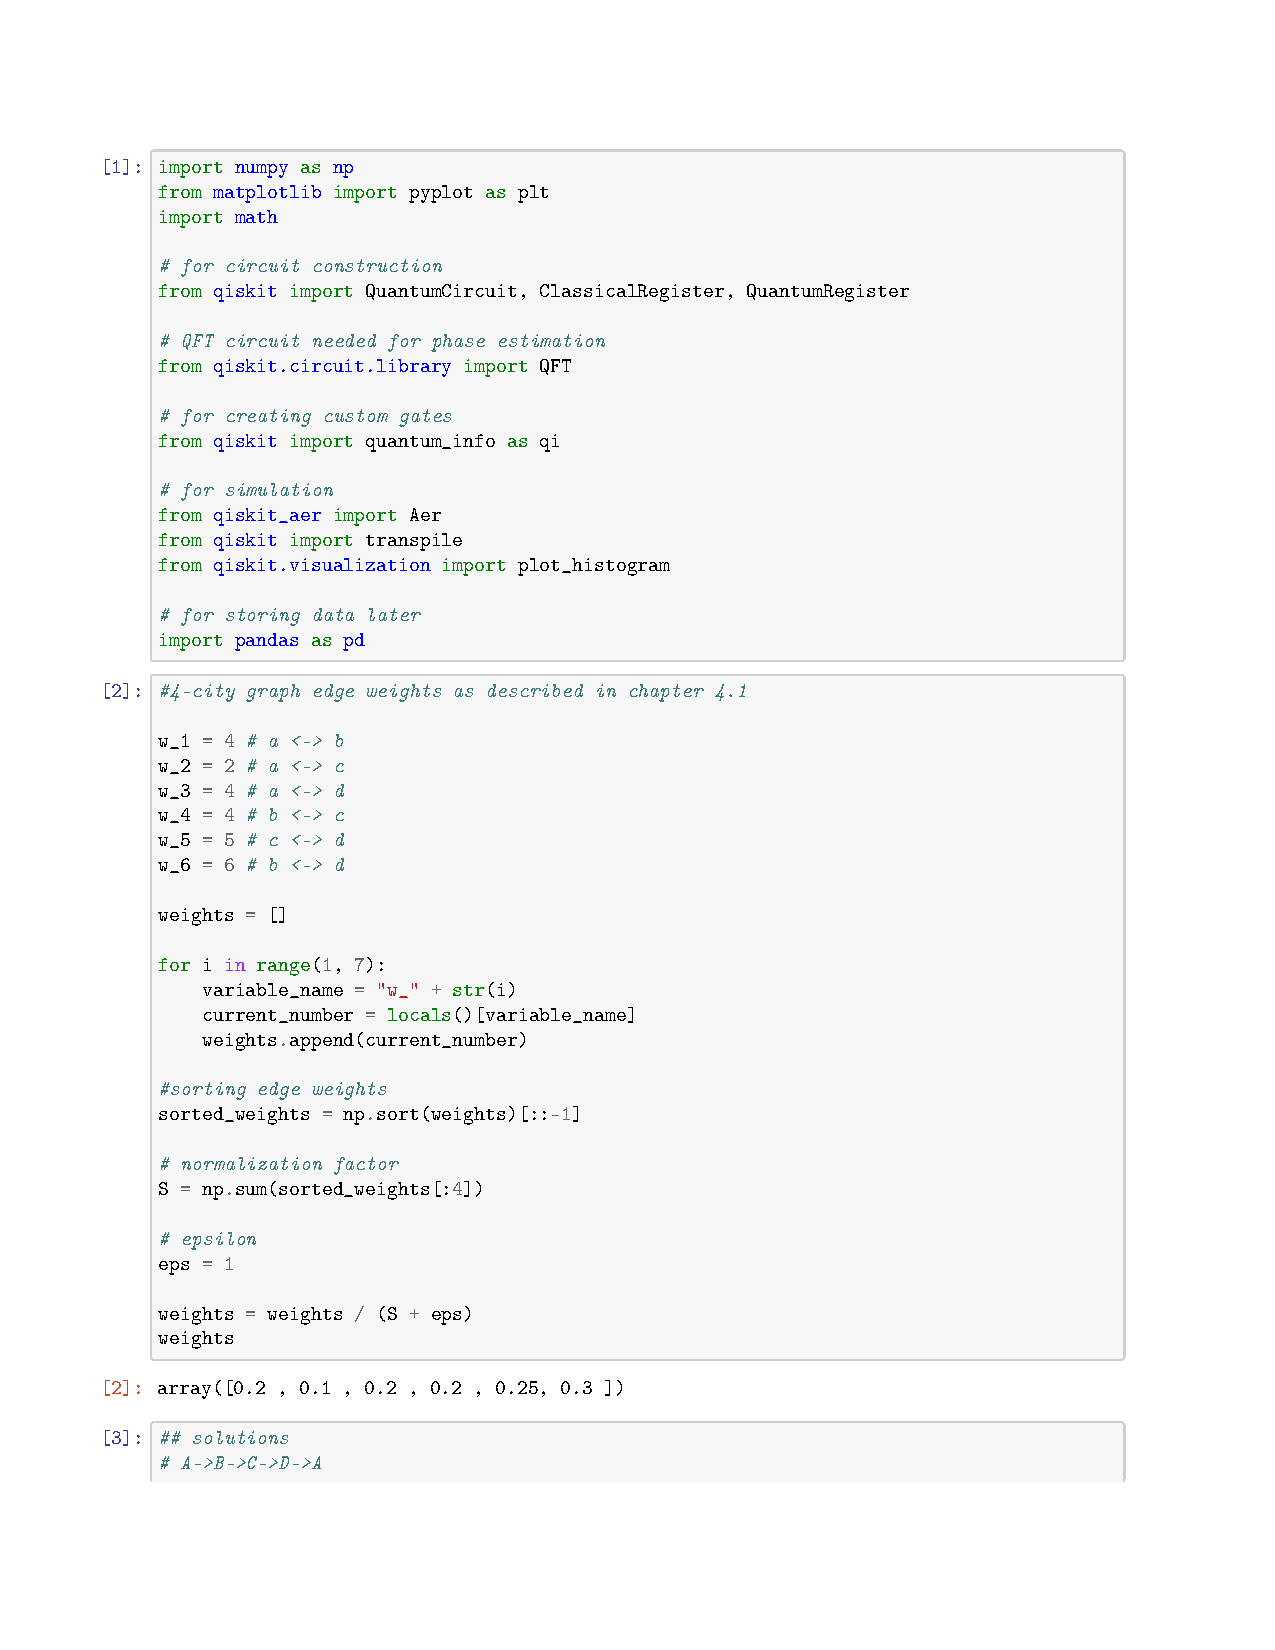
\includepdf[pages=-]{4-city-code/4-city-code.pdf}
	
	\backmatter
	
	
	\end{document}
	
	
	
\end{document}
